\documentclass[graybox, envcountchap]{svmult}
% Springer document settings
\usepackage[bottom]{footmisc}% places footnotes at page bottom

\usepackage{newtxtext}       % 
\usepackage[varvw]{newtxmath}       % selects Times Roman as basic font
%%%%%%%%%%%%%%%%%%%%%%%%%%%%%%%

% \usepackage{amssymb}
\usepackage{ntheorem}
\usepackage{amsmath}
\usepackage{enumitem}


\usepackage{graphicx}
\usepackage{color}
\usepackage{cite}
\usepackage{makeidx}


\usepackage{ascmac}
\usepackage{eclbkbox}
\usepackage{dsfont}

\usepackage{longtable}

\usepackage{url}

\usepackage{hyperref}

\usepackage{multicol}

%% --川口追加--
\makeatletter
\let\MYcaption\@makecaption
\makeatother
\usepackage{subcaption}
\captionsetup{compatibility=false}      % 必要に応じて

\makeatletter
\let\@makecaption\MYcaption
\makeatother
% ----

%%
\theoremstyle{plain}
\theoremheaderfont{\bfseries}
\theorembodyfont{\rmfamily}
\theoremseparator{\hspace{1ex}}
\theoremindent0cm
\theoremnumbering{arabic}
\theoremprework{\vspace{1ex}\begin{shadebox}\vspace{1ex}}
\theorempostwork{\vspace{-1ex}\end{shadebox}\vspace{1ex}}

%%
\theoremclass{theorem}

%%
\theoremclass{theorem}

%%
\theoremclass{theorem}


%%
\theoremstyle{break}
\theoremheaderfont{\bfseries}
\theorembodyfont{\rmfamily}
\theoremseparator{}
\theoremindent0cm
\theoremnumbering{arabic}
\theoremprework{\vspace{1.5ex}\begin{breakbox}\vspace{-0.5ex}}
\theorempostwork{\vspace{-0.5ex}\end{breakbox}\vspace{1.5ex}}

%%
\theoremstyle{nonumberplain}
\theoremseparator{\hspace{1ex}}

%%
\newtheorem{assumption}{Assumption}[section]

%%
\renewcommand{\theproblem}{}

\renewcommand{\theremark}{}


\newcommand{\red}[1]{{\color{red}#1}}
\newcommand{\blue}[1]{{\color{blue}#1}}
\newcommand{\green}[1]{{\color{green}#1}}

\DeclareMathOperator*{\argmax}{arg\,max}

\newcommand{\bm}[1]{\boldsymbol{#1}}
\newcommand{\sfT}{\mathsf{T}}

\newcommand{\advanced}{$^{\ddag}$}

\DeclareMathOperator{\sfsin}{\mathsf{sin}}
\DeclareMathOperator{\sfcos}{\mathsf{cos}}
\DeclareMathOperator{\sftan}{\mathsf{tan}}
\DeclareMathOperator{\sfarctan}{\mathsf{arctan}}

\DeclareMathOperator{\sfdiag}{\mathsf{diag}}
\DeclareMathOperator{\sfcol}{\mathsf{col}}
\DeclareMathOperator{\sfdet}{\mathsf{det}}
\DeclareMathOperator{\sfadj}{\mathsf{adj}}
\DeclareMathOperator{\sftrace}{\mathsf{trace}}

\DeclareMathOperator{\real}{\mathsf{Re}}

\DeclareMathOperator{\sfker}{\mathsf{ker}}
\DeclareMathOperator{\sfim}{\mathsf{im}}

\DeclareMathOperator{\sfdim}{\mathsf{dim}}
\DeclareMathOperator{\sfspan}{\mathsf{span}}

\DeclareMathOperator{\sfint}{\mathsf{int}}

\DeclareMathOperator*{\sfmin}{\mathsf{min}}
\DeclareMathOperator*{\sfmax}{\mathsf{max}}
\DeclareMathOperator*{\sfsup}{\mathsf{sup}}

\DeclareMathOperator{\sfsat}{\mathsf{sat}}

\newcommand{\mat}[1]{\left[\: \begin{matrix} #1 \end{matrix} \:\right]}
\newcommand{\spliteq}[1]{\begin{split} #1 \end{split}}
\newcommand{\simode}[1]{\begin{cases}  \begin{split} #1 \end{split} \end{cases}}

\newcommand{\proofend}{\hfill \rule{2mm}{3mm}}

\newcommand{\Xti}{X_i'}
\newcommand{\Xsi}{X_i}

\newcommand{\Xtone}{X_1'}
\newcommand{\XtN}{X_N'}

\newcommand{\Xt}{X'}
\newcommand{\Xs}{X}

\newcommand{\taudi}{\tau_i}
\newcommand{\taud}{\tau}

\newcommand{\Cgi}{b_i}


\newcommand{\Ifd}{I_{\rm field} }

\newcommand{\matlab}{\textsc{Matlab} }





%% --川口追加--
\newcommand{\thshift}{\theta_{12}}
\newcommand{\thshiftb}{\theta_{32}}
\newcommand{\Ysa}{\bm y_{12}}
\newcommand{\bca}{c_{12}}
\newcommand{\Ysb}{\bm y_{32}}
\newcommand{\bcb}{c_{32}}
\newcommand{\bcij}{c_{ij}}
\newcommand{\Is}{{\bm I}_{12}' }
\newcommand{\im}{\bm j}
\newcommand{\tr}{{\sf T}}

%%%%%%%%%%%%%%%%%%%%%%%%% code lines %%%%%%%%%%%%%%%%%%%%%%%%%%%%%%%%%%%%%%%%%%
\usepackage{listings}
\usepackage{xcolor}
\renewcommand{\lstlistingname}{Program}% Listing -> Algorithm
\renewcommand{\lstlistlistingname}{List of \lstlistingname s}% List of Listings -> List of Algorithms

\definecolor{codegreen}{rgb}{0,0.6,0}
\definecolor{codegray}{rgb}{0.5,0.5,0.5}
\definecolor{codepurple}{rgb}{0.58,0,0.82}
\definecolor{backcolour}{rgb}{0.95,0.95,0.92}

\lstdefinestyle{mystyle}{
    backgroundcolor=\color{backcolour},   
    commentstyle=\color{codegreen},
    keywordstyle=\color{magenta},
    numberstyle=\tiny\color{codegray},
    stringstyle=\color{codepurple},
    basicstyle=\ttfamily\footnotesize,
    breakatwhitespace=false,         
    breaklines=true,                 
    captionpos=b,                    
    keepspaces=true,                 
    numbers=left,                    
    numbersep=5pt,                  
    showspaces=false,                
    showstringspaces=false,
    showtabs=false,                  
    tabsize=2
}

\lstset{style=mystyle}


\begin{document}

\chapter{Mathematical model of electrical power systems}\label{ch:model}

In this Chapter, we explain the mathematical model of electrical power systems.
In summary, we show that the dynamics of synchronous generators can be described
by differential equations, and loads can be described by algebraic equations.
Therefore, by combining both the equations of loads and synchronous generators,
the entire electrical power system can be expressed as nonlinear
differential-algebraic equations.

The current Chapter is structured as follows. First, in Section
\ref{sec:basicele}, we introduced to the basic concept of impedance and
admittance of circuit elements and phasor representation of current and voltage
in AC circuits. Next, in Section \ref{sec:transadm}, we introduce the concept of
nodal admittance matrix, which is a mathematical model of power grids. In
Sections \ref{sec:genmod} and \ref{sec:modload}, mathematical models for
generators and loads are explained. Specifically, in Section \ref{sec:genmod},
we show that the model of a power grid composed only by generators can be
expressed as a nonlinear ordinary differential equation through Kron reduction
of the generator buses. The behavior of such an ordinary differential equation
system is shown through a numerical simulation.

\section{Foundation of AC circuit theory}\label{sec:basicele}

\subsection{Circuit elements}

The basic circuit elements used in mathematical modeling of electrical power
systems include resistors, inductors and capacitors. The relationship between
terminal voltage and terminal current of each element is presented as follows: 

\newpage
\begin{figure}[t]
  \centering
  {
    \begin{minipage}{0.3\linewidth}
      \centering
      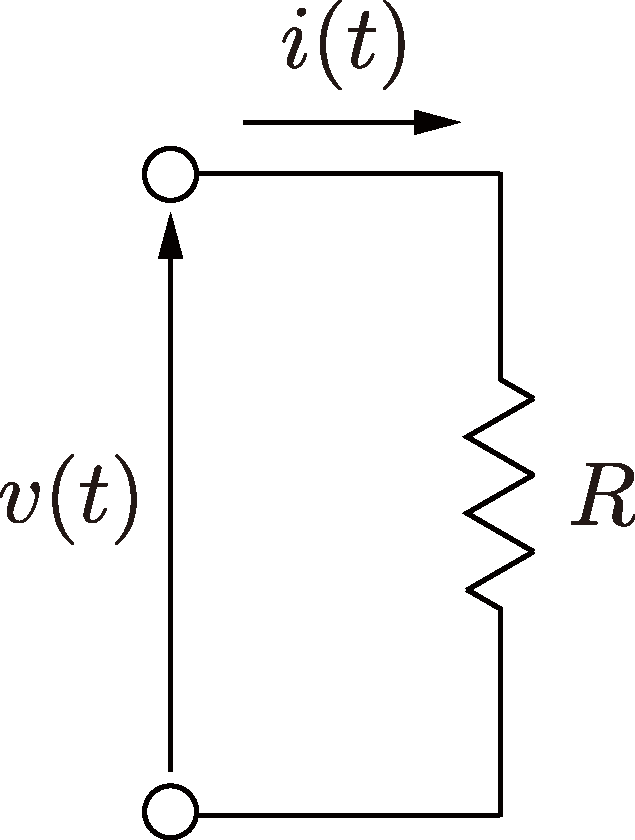
\includegraphics[width = .7\linewidth]{figs/circres2}
      \subcaption{}
      \medskip
    \end{minipage}
    \begin{minipage}{0.3\linewidth}
      \centering
      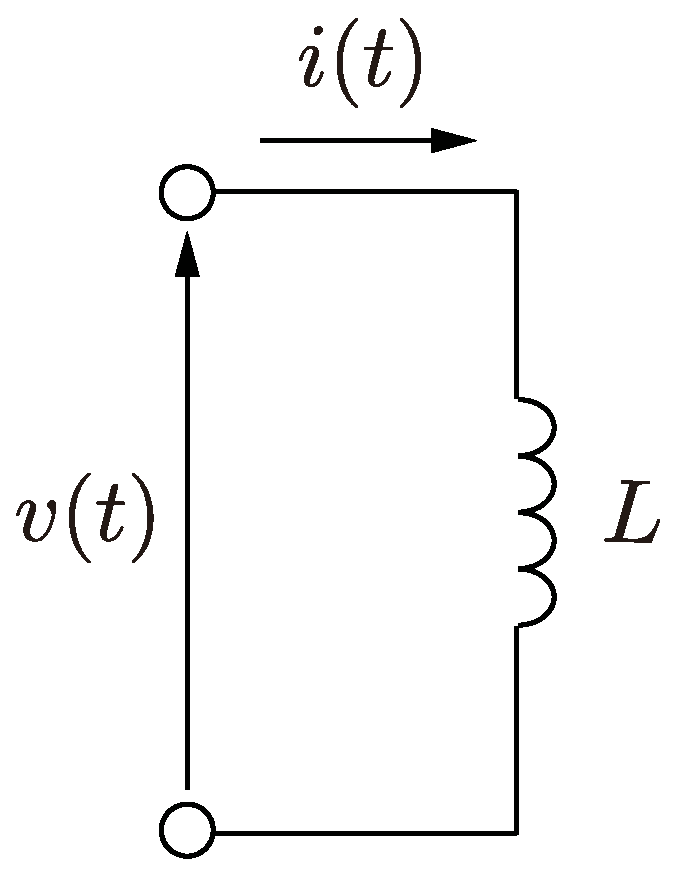
\includegraphics[width = .7\linewidth]{figs/circcoil}
      \subcaption{}
      \medskip
    \end{minipage}
    \begin{minipage}{0.3\linewidth}
      \centering
      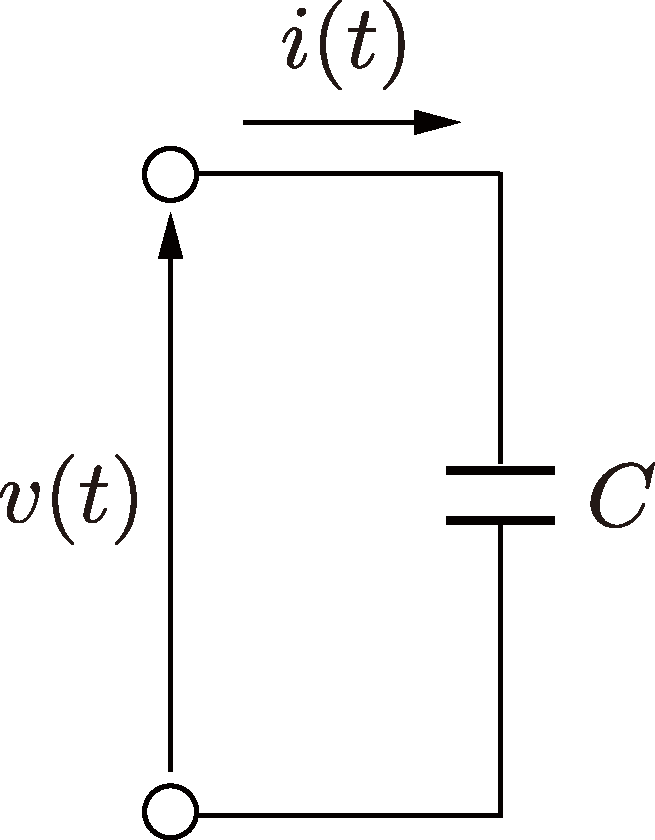
\includegraphics[width = .7\linewidth]{figs/circcond}
      \subcaption{}
      \medskip
    \end{minipage}
  }
  \medskip
  \caption{\centering Basic circuit of resistors, inductors, and
  capacitors.}
  \label{fig:basiccirc} 
  \medskip
\end{figure}

\smallskip
\begin{enumerate}[label=(\alph*)]
  \item \textbf{Resistor:} For the resistor with resistance of $R$~[$\Omega$]
  shown in \ref{fig:basiccirc}(a), the following relationship holds between the
  terminal voltage $v$~[V] and terminal current $i$~[A]:
  \begin{equation}
    v(t) = R i(t)
  \end{equation}
  where $R\geq 0$.
  \bigskip
  \item \textbf{Inductor:} For the inductor with inductance $L$~[H] shown in
  \ref{fig:basiccirc}(b), the following relationship holds between the terminal
  voltage and terminal current:
  \begin{equation}
    v(t) = L \frac{di}{dt}(t)
  \end{equation}
  where $L\geq 0$.
  \bigskip
  \item \textbf{Capacitor:} For the capacitor with capacitance $C$~[F] shown in
  \ref{fig:basiccirc}(c), the following relationship holds between the terminal
  voltage and terminal current:
  \begin{equation}
    i(t) = C \frac{dv}{dt}(t)
  \end{equation}
  where $C\geq 0$.
\end{enumerate}

\subsection{Instantaneous value and effective value}

\smallskip
\begin{enumerate}[label=(\alph*)]
  \item \textbf{Instantaneous value:} The instantaneous value of an AC quantity
  is an expression of this quantity in function of time $t$. For example, for a
  sinusoidal alternating voltage, its instantaneous value can be expressed by:
  \begin{equation}\label{eq:acvolt}
    v(t) = V_{\rm m} \sfsin (\omega t + \phi)
  \end{equation}
  where $V_{\rm m}$~[V] is the voltage amplitude, $\omega$~[rad/s] is the
  angular frequency, and $\phi$~[rad] is the phase. The sine wave period
  $T$~[s] is expressed as follows using $\omega$:
  \begin{equation}
    T:=\frac{2\pi}{\omega}
  \end{equation}
  Frequency $f$~[Hz] is expressed as its reciprocal $f:=\tfrac{1}{T}$. Due to
  the characteristics of the elements presented in Section \ref{sec:basicele},
  when the instantaneous value of voltage is a sine wave, the instantaneous
  value of the current also becomes a sine wave.
  \bigskip
  \item \textbf{Effective value:} The effective value of an AC quantity
  corresponds to the square root of the average of the square of the values over
  a period of time $T$. Because of this definition, the effective value is also
  called \textbf{RMS value} (root mean square value). For example, for the
  resistor in \ref{fig:basiccirc}(a), the average electric power consumed in one
  period can be calculated as follows:
  \begin{equation}\label{eq:efP}
    \frac{1}{T}
    \int_{t}^{t+T} v(\tau) i(\tau) d\tau = 
    \frac{1}{R}
    \Biggl( \underbrace{\frac{V_{\rm m}}{\sqrt{2}} }_{V_{\rm e}} \Biggr)^2
  \end{equation}
  where $V_{\rm e}$ is the \textbf{effective value} of voltage. The effective
  value of the current is defined in the same manner. Since the average electric
  power can be described simply by using the effective value of voltage and
  current, the effective value is often used to perform calculations for AC
  circuit. The effective value is also used for the phasor representation of
  voltage and current introduced below.
\end{enumerate}

\subsection{Phasor representation}\label{sec:intphas}
The AC voltage waveform of Equation \ref{eq:acvolt} can be represented in the
complex plane as in Figure \ref{fig:phasorrep}. In this case, $v(t)$ is
expressed by the following equation:
\begin{equation}\label{eq:Vcomp}
  v(t)= \imag \left[ V_{\rm m} e^{\bm{j}(\omega t + \phi)} \right]
\end{equation}

\begin{figure}[t]
  \centering
  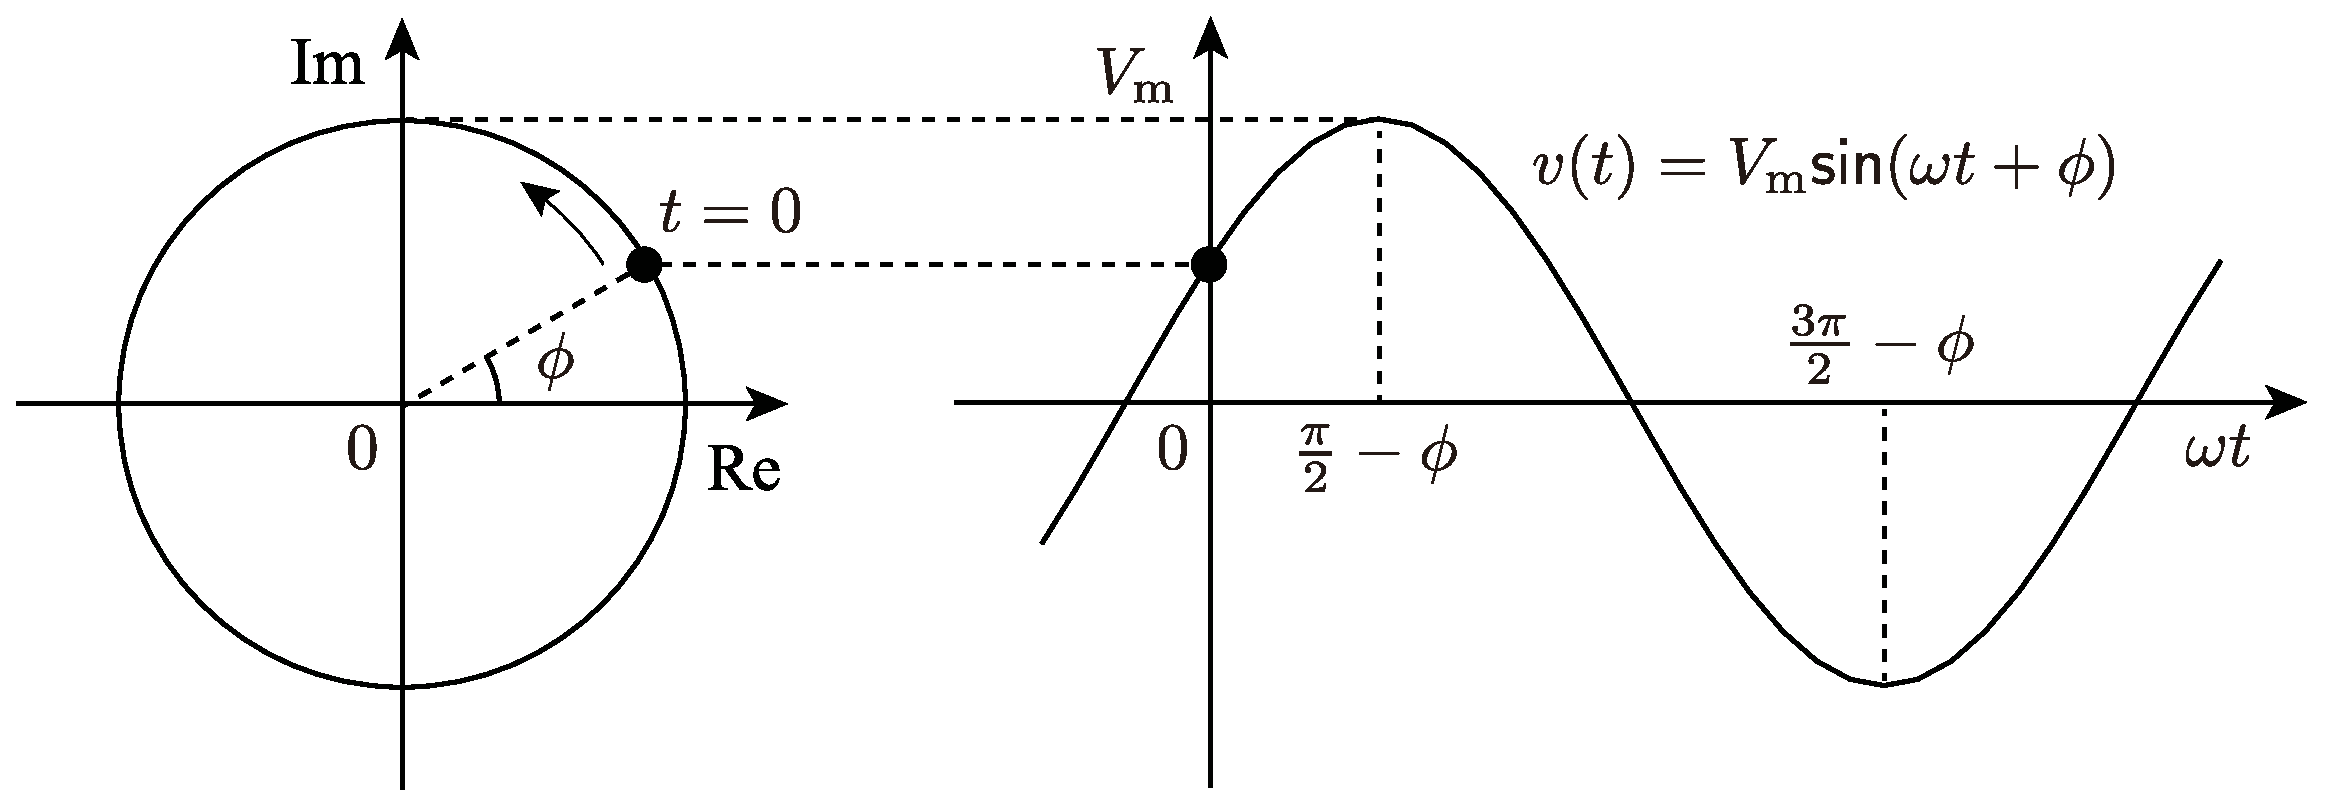
\includegraphics[width = .99\linewidth]{figs/phasorrep}
  \caption{\textbf{Complex plane representation of AC voltage}}
  \label{fig:phasorrep}
  \medskip
\end{figure}
In an electrical power system, the angular frequency $\omega$ can be considered
constant and equal to the reference angular speed. Under this assumption, the
voltage $v(t)$ of Equation \ref{eq:Vcomp} can be uniquely expressed by the phase
$\phi$, which can be derived from $\omega t$ and the amplitude $V_{\rm m}$.
Then, by using the effective value as an expression of the amplitude, we can
obtain:

\begin{equation}\label{eq:Vphasor}
  \bm{V}:= V_{\rm e} e^{\bm{j}\phi}
\end{equation}

This is called the \textbf{phasor representation} of voltage. When an electrical
power system is in a steady state, the phasor $\bm{V}$ is constant. In other
words, the absolute value $|\bm{V}|=V_{\rm e}$ and phase $\angle \bm{V}=\phi$
are constant. On the other hand, when an electrical power system is in a
transient state, the temporal changes of $|\bm{V}|$ and $\angle \bm{V}$ have to
be analyzed. The definition for the current phasor $\bm{I}$ is the same.

\subsection{Impedance and admittance}

The concept of impedance $\bm{Z}$~[$\Omega$] arises when expressing the
relationship between voltage and curring using the phasor representation
explained in Section \ref{sec:intphas}. It is equivalent to the resistance in DC
circuits, and corresponds to an opposition to alternating current. For the
typical circuit elements presented in Section \ref{sec:basicele}, the phasor
representations of their terminal voltage and current $\bm{V}$, $\bm{I}$ respect
the following relationship.

\begin{equation}
  \bm{V} = \bm{Z}\bm{I}
\end{equation}

The impedance of resistors, inductors and capacitors are, respectively:

\[
  \bm{Z}_{R}:=R,\qquad
  \bm{Z}_{L}:=\bm{j}\omega L,\qquad
  \bm{Z}_{C}:=\frac{1}{\bm{j}\omega C}
\]

Please note that the characteristics of components such as synchronous
generators and power converters may not be expressed using only constant
impedances.

The real part of impedance is called \textbf{resistance} and the imaginary part
is called \textbf{reactance}. As standard symbols, $R$~[$\Omega$] is used for
resistance and $X$~[$\Omega$] is used for reactance. In other words:

\[
  \bm{Z} = R + \bm{j} X
\]
The reciprocal $\bm{Z}^{-1}$ of impedance is called \textbf{admittance}.
As a standard symbol, $\bm{Y}$~[S] is used.
In addition, the real part of admittance is called \textbf{conductance} and the imaginary part is called \textbf{susceptance}.
As a standard symbol, $G$~[S] is used for conductance and $B$~[S] is used for susceptance.
In other words:
\[
\bm{Y} = G + \bm{j} B
\]

The reading of each physical unit presented so far is, V: volt, A: ampere,
$\Omega$: ohm, H: henry, F: farad, rad: radian, s: second, Hz: hertz, and S:
siemens.

\section{Admittance matrix: representation of interaction between connected
devices}\label{sec:transadm}

\subsection{Fundamentals of modeling of power grids}
In this section we derive the \textbf{admittance matrix} of a power grid, which
expresses the interaction between the devices connected to an electrical power
system 

We derive the \textbf{admittance matrix} of a power grid that shows the
interaction of equipment connected to an electrical power system using a basic
transmission line model. The admittance matrix is derived from Ohm's law and
Kirchhoff's laws for each bus bar and the transmission lines that connect them.
Depending on the literature, the bus bar may also be called a \textbf{node} or
\textbf{bus}. In this book, the bus bar is shown with a thick line in the
diagram of an electrical power system.  The bus bar is a conductor where the end
of the transmission line has been collected. The thin line that connects the bus
bar represents the transmission line.

\begin{figure}[t]
  \centering
  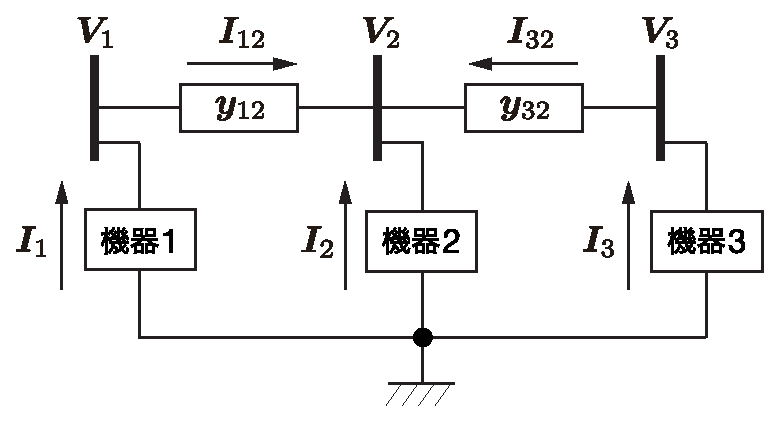
\includegraphics[width = .60\linewidth]{figs/3busex}
  \medskip
  \caption{\textbf{Power system model composed of three bus bars}}
  \label{fig:3busex}
  \medskip
\end{figure}

\begin{example}{\textbf{Admittance matrix of a power grid}}\label{ex:derY}

  Let us consider a simple electrical power system consisting of three bus bars as
  shown in Fig. \ref{fig:3busex}. Assume that to each bus there is a device
  connected. In this book, the word "device" refers to synchronous generators and
  loads. \footnote{In this book, we analyze only load and generators, however,
  when considering solar generators, wind generators and batteries, these are also
  classified as "devices".} In addition, in an electrical power system model
  circuit such as that shown in \ref{fig:3busex}, the connection to ground is
  often omitted for simplification.

  Below, the voltage phasor of bus bar $i$ with respect to the ground is expressed
  as $\bm{V}_i \in \mathbb{C}$, and the current phasor flowing from the device to
  the bus bar $i$ is expressed as $\bm{I}_i \in \mathbb{C}$. The voltage and
  current phasors are unknown variables, therefore it is necessary to find an
  equation governed by the power grid that establishes a relationship between the
  current phasor $(\bm{I}_1,\bm{I}_2,\bm{I}_3)$ and the current phasor
  $(\bm{V}_1,\bm{V}_2,\bm{V}_3)$ of the bus bars. For this purpose, we define the
  admittance matrix of the power grid. 

  The admittance of a transmission line that connects bus bars $i$ and $j$ is
  expressed as $\bm{y}_{ij}\in \mathbb{C}$, with $y_{ij}$ being known variables
  for every pair of bus bars $ij$. Additionally, the current phasor that flows in
  each transmission line is expressed as $\bm{I}_{ij}\in \mathbb{C}$, where
  $\bm{y}_{ij}$ and $\bm{y}_{ji}$ are equal. In addition, the sign for
  $\bm{I}_{ij}$ is positive for an arbitrarily determined direction, and
  $\bm{I}_{ji} = -\bm{I}_{ij}$ are equal. The current phasor of this transmission
  line is an intermediate variable that describes the physical relationship of the
  current phasor and voltage phasor of the bus bars. Specifically, if the sign of
  the current phasor is defined positive for the direction indicated by the arrows
  in Fig. \ref{fig:3busex}, the following relationship can be obtained by applying
  the Ohm's law:

  \begin{equation*}
  \bm{I}_{12}=\bm{y}_{12}(\bm{V}_{1}-\bm{V}_{2}),\qquad
  \bm{I}_{32}=\bm{y}_{32}(\bm{V}_{3}-\bm{V}_{2})
  \end{equation*}


  According to Kirchhoff's first law (current law), since the sum of all current
  on each bus bar is 0, the following relationship is obtained for bus bar 1 to
  bus bar 3.

  \begin{equation*}
  \bm{I}_{1}-\bm{I}_{12}=0,\qquad
  \bm{I}_{2}+\bm{I}_{12}+\bm{I}_{32}=0,\qquad
  \bm{I}_{3}-\bm{I}_{32}=0
  \end{equation*}

  Note that Kirchhoff's first law states that the sum of inflow currents and the
  sum of outflow currents are equal at the point where an electric circuit
  branches. By replacing the variables $\bm{I}_{ij}$ by the previously calculated
  relationship $\bm{I}_{i} = \bm{y}_{ij}(\bm{V}_{1}-\bm{V}_{2})$, we can find the
  following vectorized version of the Ohm's law:

  \begin{equation}\label{eq:exY}
    \mat{
    \bm{I}_1\\
    \bm{I}_2\\
    \bm{I}_3\\
    }
    =
    \mat{
    \bm{y}_{12} & -\bm{y}_{12} & 0\\
    -\bm{y}_{12} & \bm{y}_{12}+\bm{y}_{32} & -\bm{y}_{32}\\
    0 & -\bm{y}_{32} & \bm{y}_{32}
    }
    \mat{
    \bm{V}_1\\
    \bm{V}_2\\
    \bm{V}_3\\
    }
  \end{equation}

  The complex matrix obtained in this manner is the admittance matrix of the power
  grid. Since each transmission line is usually expressed as a circuit with an
  equivalent resistance and inductance, the real part (conductance) of the
  admittance of the transmission line $\bm{y}_{ij}$ is non-negative, and the
  imaginary part (susceptance) is non-positive. Specifically, the imaginary part
  is usually negative (non-zero).
\end{example}

Below, we consider an electrical power system connected with $N$ bus bars. Then,
the admittance matrix $\bm{Y} \in \mathbb{C}^{N \times N}$ of the power grid
gives the following relationship to the current phasor
$(\bm{I}_1,\ldots,\bm{I}_N)$ and voltage phasor $(\bm{V}_1,\ldots,\bm{V}_N)$ of
the bus bars.
\begin{equation}\label{eq:ohmY}
\mat{
  \bm{I}_1\\
  \vdots\\
  \bm{I}_N
}
 =
\underbrace{
\mat{
  \bm{Y}_{11} & \cdots & \bm{Y}_{1N}\\
  \vdots & \ddots & \vdots\\
  \bm{Y}_{N1} & \cdots & \bm{Y}_{NN}
}
}_{\bm{Y}}
\mat{
  \bm{V}_1\\
  \vdots\\
  \bm{V}_N
}
\end{equation}
Equation \ref{eq:ohmY} can be considered a mathematical model of the power grid
that expresses interactions between inputs and outputs of devices connected to a
bus bar.  Specifically, if we consider the voltage phasor $\bm{V}_i$ as the
output from the device $i$ to the electrical power system, and current phasor
$\bm{I}_i$ as the input from the electrical power system to the device $i$,
$\bm{I}_i$ can be expressed as a linear combination of output from the other
devices:

\begin{equation*}
 \bm{I}_i = \bm{Y}_{i1}  \bm{V}_1 + \cdots +\bm{Y}_{iN}  \bm{V}_N
\end{equation*}

The real part and imaginary parts of the admittance matrix are called the
\textbf{conductance matrix} and \textbf{susceptance matrix}, respectively.

The simultaneous equations \ref{eq:ohmY} provide partial information about the
current and voltage phasors of the bus bars, such that the current and voltage
phasors of each bus bar, $(\bm{I}_1,\ldots,\bm{I}_N)$ and
$(\bm{V}_1,\ldots,\bm{V}_N)$, cannot be uniquely determined. To uniquely
determine the steady and transient behaviors of the current and voltage phasors
of every bus bar, the local relationship between $\bm{I}_i$ and $\bm{V}_i$ of
each bus bar must be separately determined.

This localized relationship expresses the characteristics of the devices
connected to the bus bars and can be considered mathematical models that express
the input-output relationship of each device. Specific mathematical models of
synchronous generators and loads will be described in detail in Section
\ref{sec:genmod} and beyond.

\begin{figure}[t]
\centering
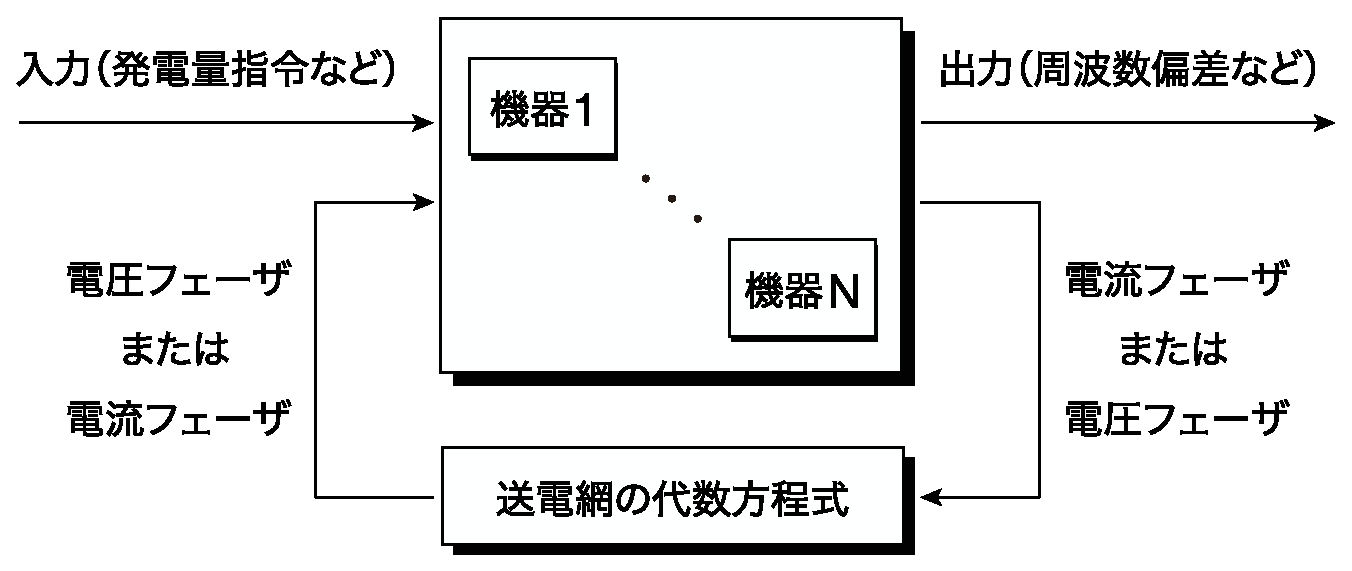
\includegraphics[width = .80\linewidth]{figs/overview}
\medskip
\caption{
  \textbf{Schematic diagram of a power system model}
}
\label{fig:overviewpwmod}
\medskip
\end{figure}


\begin{equation}\label{eq:ohmZ}
 \mat{
  \bm{V}_1\\
  \vdots\\
  \bm{V}_N
}
=
\underbrace{
\mat{
  \bm{Z}_{11} & \cdots & \bm{Z}_{1N}\\
  \vdots & \ddots & \vdots\\
  \bm{Z}_{N1} & \cdots & \bm{Z}_{NN}
}
}_{\bm{Z}}
\mat{
  \bm{I}_1\\
  \vdots\\
  \bm{I}_N
}
\end{equation}
If the admittance matrix $\bm{Y}$ in Equation \ref{eq:ohmY} is nonsingular,
$\bm{Z}=\bm{Y}^{-1}$, however $\bm{Y}$ is not always nonsingular. For example,
if the admittance matrix of Equation \ref{eq:exY} is not nonsingular, the
following holds:

\[
\bm{V}_1=\bm{V}_2=\bm{V}_3
\qquad  \Longrightarrow \qquad 
\bm{I}_1=\bm{I}_2=\bm{I}_3=0
\]

The singularity of this admittance matrix indicates that when all current
phasors of each bus bar are zero, all voltage phasors are the same; however,
this value cannot be uniquely determined. Nevertheless, there is rarely any need
to pay attention to the singularity of the admittance matrix within the scope of
general analysis.

\begin{figure}[t]
\centering
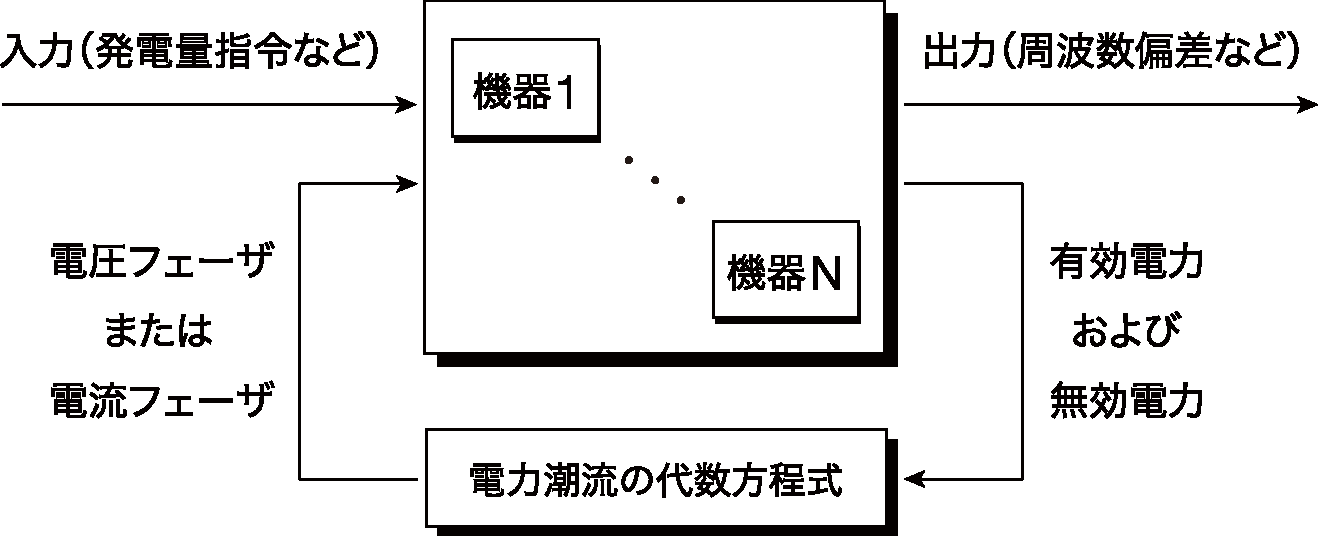
\includegraphics[width = .80\linewidth]{figs/overviewPQ}
\medskip
\caption{\textbf{Schematic diagram of a power system model}}
\label{fig:overviewpwmodPQ}
\medskip
\end{figure}

In addition, active power $P_i \in \mathbb{R}$ and reactive power $Q_i \in
\mathbb{R}$ provided from device $i$ to bus bar $i$ are defined by: 

\[
  P_i := \operatorname{Re} \left[ \bm{V}_i \overline{\bm{{I}} }_i \right], \qquad
  Q_i := \operatorname{Im} \left[ \bm{V}_i \overline{\bm{{I}} }_i \right]
\]

In other words, the following relationship holds between active power, reactive
power, bus bar voltage phasor, and bus bar current phasor.

\begin{equation}\label{eq:defPQVIi}
  P_i+\bm{j}Q_i = \bm{V}_i \overline{\bm{{I}} }_i
\end{equation}

Then, by rearranging Equation \ref{eq:ohmY}, it is possible to obtain a power
system model in which the active and reactive power supplied to the bus bar is
the output of the device.

\begin{equation}\label{eq:ohmpf}
  \begin{aligned}
    P_i &= \sum_{j=1}^{N}
    \operatorname{Re} \left[ \overline{\bm{Y}}_{ij} \bm{V}_i \overline{\bm{V}}_j 
    \right] \\
    Q_i &= \sum_{j=1}^{N}
    \operatorname{Im} \left[
    \overline{\bm{Y}}_{ij} \bm{V}_i \overline{\bm{V}}_j 
    \right]
  \end{aligned}
  \qquad
  i \in \{1,\ldots, N\}
\end{equation}

Equation \ref{eq:ohmpf} is a simultaneous equation that expresses the electric
power flow in each bus bar. Figures \ref{fig:overviewpwmod} and
\ref{fig:overviewpwmodPQ} are equivalent electrical power system models, but
they can be used alternatively according to the analysis puropse.

\subsection{Power grid model with capacitance to ground}\label{sec:transmodc}

In short transmission lines, the model from the example \ref{ex:derY} can be
used; however, in medium transmission lines that exceed 50 km, the capacitance
to ground (capacitance component) created between the transmission lines and the
ground cannot be ignored. 

When the capacitance to ground, a transmission line is often represented as a
$\pi$-type equivalent circuit as shown in Figure \ref{fig:lines}. In Figure
\ref{fig:lines}, a transmission line connecting the bus bars 1 and 2 is shown,
where $\omega_0$ is the system frequency and $c_{12}$ is the capacitance to
ground. Using this representation of transmission line, the admittance of the
power grid is obtained as follows.

\begin{figure}[t]
  \centering
  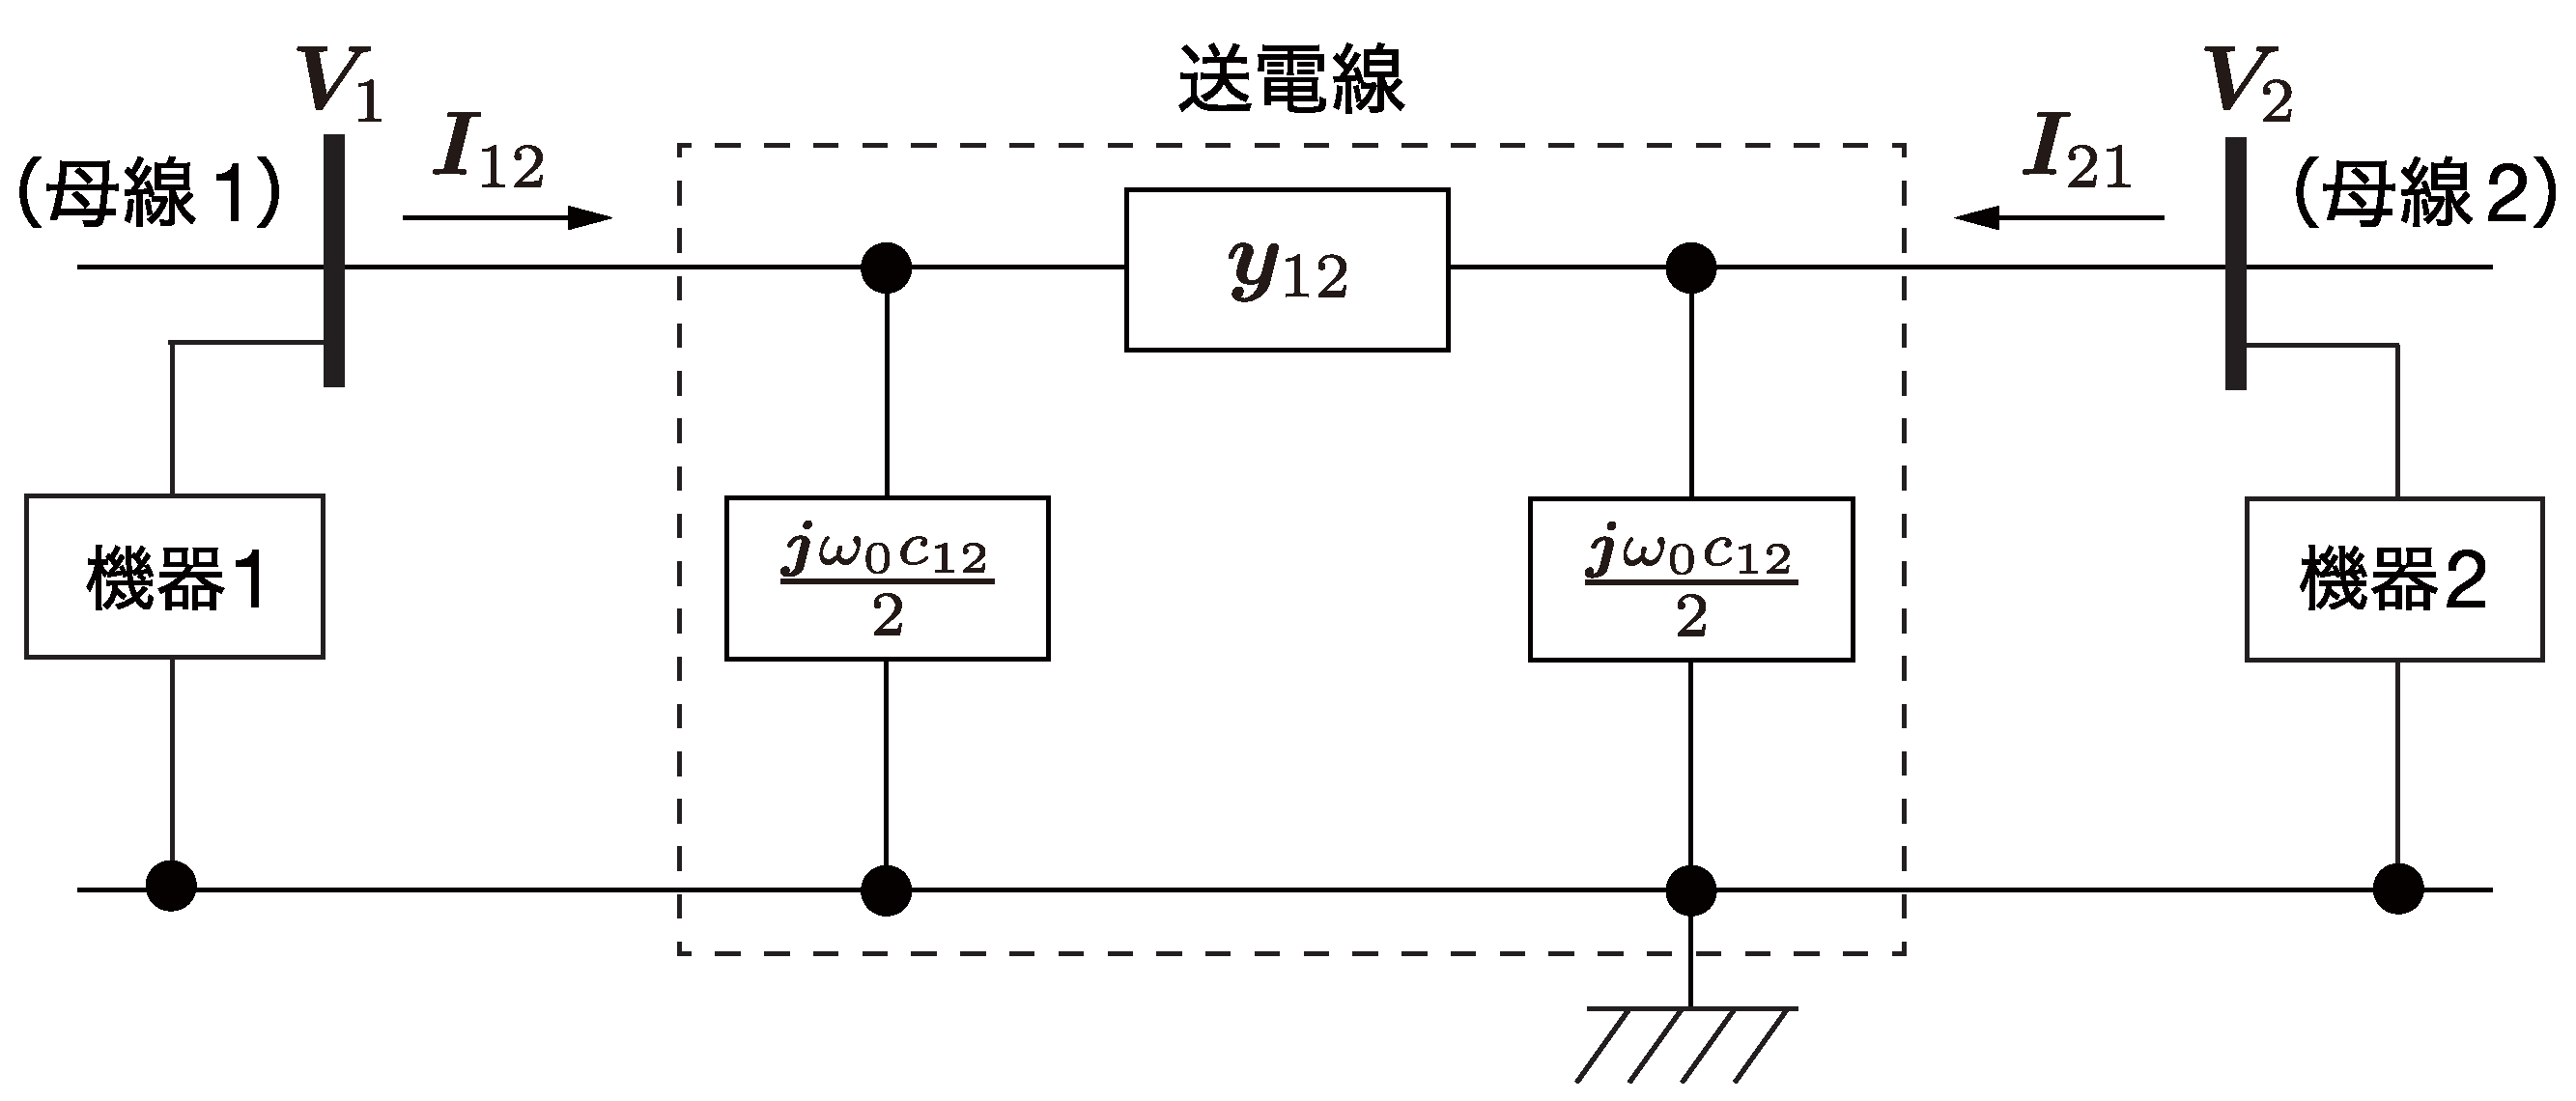
\includegraphics[width = .85\linewidth]{figs/line_pix3}
  \medskip
  \caption{\textbf{$\pi$-type circuit model of a transmission line with ground capacitance}\\
  \centering(Transmission lines with end points at bus bars 1 and 2)}
  \label{fig:lines} 
  \medskip
\end{figure}

\begin{example}{\textbf{Admittance matrix for the transmission line in a
$\pi$-type circuit}}\label{ex:pitypeY}
  
  For an electrical power system similar to Example \ref{ex:derY}, let's derive
  the admittance matrix when the transmission line is expressed by a $\pi$-type
  equivalent circuit. First, let's consider the relationship of the current
  phasors $\bm I_{12}$, $\bm I_{21}$, flowing from the bus bars, and the voltage
  phasors $\bm V_1$, $\bm V_2$ of the bus bars of a transmission line with bus
  bars 1 and 2 as end points, as illustrated in Figure \ref{fig:lines}. Then,
  please note that, unlike in Example \ref{ex:derY}, $\bm I_{21}$ is different
  from $-\bm I_{12}$. If the current flowing through the transmission line with 
  admittance $\Ysa$ from left to right is expressed as $\Is$, the following
  equations are obtained from the Kirchhoff's laws:
  
  \begin{equation*}
      \bm I_{12} = \frac{\bm{j} \omega_0 \bca}{2} \bm V_1 + \Is ,\qquad
      \frac{\bm{j} \omega_0 \bca}{2} \bm V_2 = \bm I_{21} + \Is
  \end{equation*}

  Moreover, by using the Ohm's law: 

  \begin{equation*}
    \Is = \Ysa(\bm V_1-\bm V_2)
  \end{equation*}

  By replacing $\Is$ and rearranging the equations, we obtain:

  \begin{equation*}
    \mat{
      \bm I_{12} \\ \bm I_{21}
    } = \mat{
      \Ysa +  \tfrac{\bm{j} \omega_0 \bca}{2} & -\Ysa \\
      -\Ysa & \Ysa+  \tfrac{\bm{j} \omega_0 \bca}{2}
    }
    \mat{
      \bm V_1\\\bm V_2
    }
  \end{equation*}

  The following is true for the transmission line that uses bus bar 2 and bus
  bar 3 as end points:

  \begin{equation*}
    \mat{
      \bm I_{32} \\ \bm I_{23}
    } = \mat{
      \Ysb + \tfrac{\bm{j} \omega_0 \bcb}{2} & -\Ysb \\
      -\Ysb & \Ysb+ \tfrac{\bm{j} \omega_0 \bcb}{2}
    }
    \mat{
      \bm V_3 \\ \bm V_2
    }
  \end{equation*}

  Therefore, by using:

  \begin{equation*}
    \bm{I}_{1}-\bm{I}_{12}=0,\qquad
    \bm{I}_{2}-\bm{I}_{21}-\bm{I}_{23}=0,\qquad
    \bm{I}_{3}-\bm{I}_{32}=0
  \end{equation*}

  The admittance matrix of the power grid can be obtained as: 

  \begin{equation*}%\label{eq:Ypitype}
    \mat{
    \bm{I}_1\\
    \bm{I}_2\\
    \bm{I}_3\\
    }
    =
    \mat{
    \bm{y}_{12} + \tfrac{\bm{j} \omega_0 \bca}{2} & -\bm{y}_{12} & 0\\
    -\bm{y}_{12} & \hspace{-3mm} \bm{y}_{12}+\bm{y}_{32} + \tfrac{\bm{j} \omega_0 (\bca+\bcb)}{2} & -\bm{y}_{32}\\
    0 & -\bm{y}_{32} & \hspace{-3mm} \bm{y}_{32}+ \tfrac{\bm{j} \omega_0 \bcb}{2}
    }
    \mat{
    \bm{V}_1\\
    \bm{V}_2\\
    \bm{V}_3\\
    }
  \end{equation*}

 This is consistent with Equation \ref{eq:exY} when $\bca$ and $\bcb$ are zero.
\end{example}

\subsection{Mathematical properties of the admittance matrix}\label{sec:admathp}

In this book, we assume power grids that are connected; in other words, there is
at least one route connecting two arbitrarily chosen bus bar. For unconnected
power grids, the connected parts can be independently discussed. In Figure
\ref{fig:congraph}, the nodes (circles) correspond to the bus bars and the edges
(black lines) correspond to the transmission lines.

In the power grid model of Example \ref{ex:derY} where the capacitance to ground
is ignored, the admittance matrix is expressed as $\bm{Y}_0 \in
\mathbb{C}^{N\times N}$. The real and imaginary parts of $\bm{Y}_0$; in other
words, the conductance and susceptance matrices, are expressed as:

\[
  G_0:=\operatorname{Re} [\bm{Y}_0] ,\qquad
  B_0:=\operatorname{Im} [\bm{Y}_0]
\]

These matrices have the following properties. First, the sum of elements in all
row vectors of these matrices is equal to zero. This is expressed by the
following equations, where $\mathds{1}\in \mathbb{R}^N$ is a vector which all
elements are equal to one:

\begin{subequations}\label{eq:Y0prop}
\begin{equation}\label{eq:Y0ker}
  \bm{Y}_0 \mathds{1} =0
  \qquad
  \Longleftrightarrow
  \qquad
  G_0\mathds{1} =0,\qquad
  B_0\mathds{1} =0
\end{equation}

Furthermore, since the conductance is non-negative and the susceptance is
negative in each transmission line, the conductance matrix is positive
semi-definite and the susceptance matrix is negative semi-definite; in other
words: 

\begin{equation}\label{eq:Y0}
  G_0 =G_0^{\sfT} \succeq 0,\qquad
  B_0 = B_0^{\sfT} \preceq 0
\end{equation}

Specifically, based on the fact that the connectivity of the power grid and the
susceptance of the transmission line are non-zero, the multiplicity of the zero
eigenvalue of $B_0$ is derived to be 1. This can also be expressed as:

\begin{equation}\label{eq:Y0eig}
  \sfker B_0 = \sfspan \{ \mathds{1} \}
\end{equation}

Under the graph theory perspective, $-B_0$ is called a \textbf{graph Laplacian}
of a strongly connected weighted undirected graph. The multiplicity of the zero
eigenvalue in a graph Laplacian being 1 is a requirement for the corresponding
undirected graph to be strongly connected \cite{mesbahi2010graph}.

\end{subequations}

\begin{figure}[t]
  \centering
  {
  \begin{minipage}{0.42\linewidth}
    \centering
    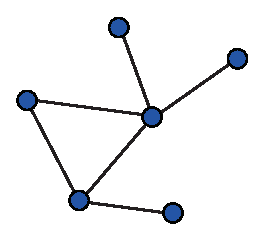
\includegraphics[width = .6\linewidth]{figs/congraph}
    \medskip
    \subcaption{Connected graph}
    \label{fig:congraph} 
  \end{minipage}
  \begin{minipage}{0.42\linewidth}
    \centering
    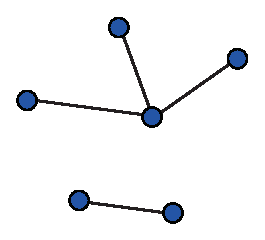
\includegraphics[width = .6\linewidth]{figs/notcongraph}
    \medskip
    \subcaption{Unconnected graphs}
    \label{fig:notcongraph} 
  \end{minipage}
  }
\medskip
\caption{\textbf{Connected and disconnected graphs} \\ \centering(Connected
graph and unconnected graph)}
\label{fig:congraphab} 
\medskip
\end{figure}

Furthermore, when considering a $\pi$-type equivalent circuit for the
transmission lines like in Example \ref{ex:pitypeY}, a non-negative value is
added to the diagonal element of the susceptance matrix $B_0$. In other words,
the admittance matrix for the power grid model in Examples \ref{ex:derY} and
\ref{ex:pitypeY} is expressed as:

\begin{equation}\label{eq:Ypig}
  \bm{Y} = G_0 + \bm{j} \left( B_0 + \sfdiag( \Cgi )_{i \in \{1,\ldots,N\}} \right)
\end{equation}
where $ \Cgi $ is a non-negative constant equivalent to capacitance to ground,
and the conductance $G_0$ and the susceptance $B_0$ matrices satisfy Equation
(\ref{eq:Y0prop}).

\section{Mathematical model of synchronous generators}\label{sec:genmod}

\subsection{Classification of generator models based on the level of detail}

In electrical power system engineering, different synchronous generator models
with different levels of detail, such as the consideration of the field and
damper windings, have been used to analyze the stability of electrical power
systems [4, 5, 8, 9]. Here, we present four types of models.

\smallskip
\begin{enumerate}[label=\textbf{(\alph*)}]
  \item \textbf{Park model} The Park model, also called \textbf{complete model},
  is a model with a high level of details that considers the change in magnetic
  flux in the stator and field and damper windings.  It consists of a
  two-dimensional linear differential equation (swing equation) that expresses
  the mechanical dynamic characteristics of the rotor of the generator, and a
  five to seven-dimensional nonlinear differential equation that expresses the
  magnetic flux changes in the stator, field winding, and damper winding.  The
  dimension of the latter differential equation that expresses changes in
  magnetic flux varies based on the number of windings to consider and the
  setting of variables. 

  The active and reactive power, which represent the electrical output of a
  generator, are nonlinear functions of the internal state of the generator. The
  models used in Japanese works consider a type of damper winding on the d-axis
  and two types of damper windings on the q-axis in addition to field winding on
  the d-axis [8].  When there is only one type of damper winding on the q-axis, if
  the constant is set appropriately, there are no issues in terms of practical
  use.
  \bigskip
  \item \textbf{Two-axis model} It is a model that approximates the differential
  equations to the algebraic equation, assuming that the time constants of the
  dynamic response of the magnetic flux change in the stator and damper winding
  are sufficiently small [9. Section 5.4]. It consists of a two-dimensional
  swing equation and a two-dimensional nonlinear differential equation
  expressing the magnetic flux change in the field and damper windings.
  Generally, the dynamic response of the magnetic flux change in the stator and
  damper winding are sufficiently fast; thus, the behavior of the Park model is
  generally well simplified.
  \bigskip
  \item \textbf{One-axis model} In contrast to the two-axis model, the one-axis
  model, also called \textbf{transient model}, is obtained under the assumption
  that the time constant of the magnetic flux change in the damper winding is
  sufficiently small [10-12]. It consists of a two-dimensional swing equation
  and a one-dimensional nonlinear differential equation that expresses the
  magnetic flux change in the field winding. In this book, we use a one-axis
  model to perform analysis.The process of deriving a one-axis model from the
  Park model is explained in \cite[Section 5]{sauer2017power} and \cite[Section
  4.15]{anderson2008power}.
  \bigskip
  \item \textbf{Classical model} It is amodel that ignores the magnetic flux
  changes in the field and damper windings. It consists of a two-dimensional
  linear swing equation and the active and reactive power are nonlinear
  functions of the internal states of the generator. This model is currently
  widely used to analyze the oscillatory and synchronization phenomena of
  electrical power systems [10-14].
\end{enumerate}

\subsection{Mathematical expression of the one-axis model}\label{sec:genfund}
\smallskip
\begin{enumerate}[label=\textbf{(\arabic*)}]
  \item \textbf{Expressing the relationship of current and voltage with the
  internal state of the generator as an intermediate variable}

  If the interval voltage of a generator $i$ connected to a bus bar $i$ is
  $E_i$, and the rotor angle relative to a coordinate system that rotates with
  angular speed $\omega_0$ is $\delta_i$, the following relationship holds for
  the voltage phasor $\bm{V}_i$ of the bus bar $i$ and for the current phasor
  $\bm{I}_i$ flowing from the generator to the bus bar $i$:
  \begin{subequations}\label{eq:phVIs}
    \begin{equation}\label{eq:phVI}
      \bm{I}_i  = \frac{1}{ \bm{j} \Xti } \left(E_i e^{\bm{j} \delta_i} - \bm{V}_i \right)
    \end{equation}
    \begin{figure}[t]
    \centering
    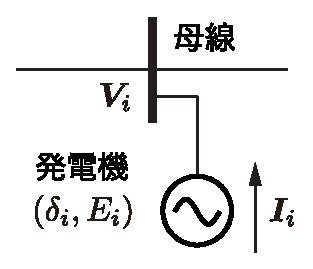
\includegraphics[width = .25\linewidth]{figs/generatorbus}
    \medskip
    \caption{\textbf{Generator connected to bus bar}}
    \label{fig:generatorbus}
    \medskip
    \end{figure}
    where $\Xti$ is the transient reactance of the generator.
    Figure \ref{fig:generatorbus} illustrates the bus bar and current and voltage
    phasors. The connection to ground is omitted from the figure.

  $\delta_i$ and $E_i$ in Equation \ref{eq:phVI} are intermediate variables
  representing the internal state of the generator $i$, and they provide with a
  dynamic relationship between $\bm{I}_i$ and $\bm{V}_i$.  In other words, from
  the perspective of control systems engineering, Equation \ref{eq:phVI} uses
  $\delta_i$ and $E_i$ as internal states, and can be interpreted as an “output
  equation” of a generator $i$, when $\bm{I}_i$ is the output from the generator
  to the electrical power system and $\bm{V}_i$ is the input from the electrical
  power system to the generator. Alternatively, we can consider $\bm{V}_i$ as
  the output and $\bm{I}_i$ as the input. Details will be discussed later. By
  multiplying both sides of the Equation \ref{eq:phVI} with $e^{- \bm{j}\delta}$
  and evaluating its real and imaginary parts separately, we find:
    \begin{equation}\label{eq:phVIsincos}
      \spliteq{
        |\bm{V}_i| \sfsin (\delta_i -\angle \bm{V}_i)  &= 
        \Xti |\bm{I}_i| \sfcos (\delta_i -\angle \bm{I}_i), \\
        |\bm{V}_i| \sfcos (\delta_i -\angle \bm{V}_i)  &= 
        E_i - \Xti |\bm{I}_i| \sfsin (\delta_i -\angle \bm{I}_i)
      }
    \end{equation}
  \end{subequations}

  Active power $P_i$ provided from the generator $i$ to the bus bar $i$ and can
  be expressed as:

  \begin{equation*}
    \spliteq{
      P_i&=\real \left[ \bm{V}_i \overline{ \bm{I} }_i \right]  
      \\
      &= 
      \real \left[ |\bm{V}_i|e^{ -\bm{j} (\delta_i -\angle \bm{V}_i )} \overline{|\bm{I}_i | e^{ -\bm{j} ( \delta_i - \angle \bm{I}_i)} } \right]
      \\
      &=
      |\bm{V}_i| |\bm{I}_i| 
      \sfcos(\delta_i -\angle \bm{V}_i) \sfcos(\delta_i -\angle \bm{I}_i) \\
      & \hspace{10em} +|\bm{V}_i| |\bm{I}_i|
      \sfsin(\delta_i -\angle \bm{V}_i) \sfsin(\delta_i -\angle \bm{I}_i)
    }
  \end{equation*}

  Similarly, reactive power $Q_i$ can be expressed as:

  \begin{equation*}
  \spliteq{
    Q_i&=\imag \left[ \bm{V}_i \overline{ \bm{I} }_i \right] \\
    &=
    |\bm{V}_i| |\bm{I}_i | \sfcos(\delta_i -\angle \bm{V}_i ) \sfsin(\delta_i -\angle \bm{I}_i) \\
    & \hspace{10em} - |\bm{V}_i| |\bm{I}_i| \sfsin(\delta_i -\angle \bm{V}_i ) \sfcos(\delta_i -\angle \bm{I}_i)
  }
  \end{equation*}

  Thus, by replacing the current phasor using the Equation \ref{eq:phVIsincos},
  the following can be obtained:

  \begin{equation}\label{eq:PiQis}
    \spliteq{
      P_i & =  \frac{E_i |\bm{V}_i |}{ \Xti } \sfsin(\delta_i -  \angle \bm{V}_i), \\
      Q_i & =  \frac{E_i |\bm{V}_i |}{ \Xti } \sfcos (\delta_i - \angle \bm{V}_i) - \frac{|\bm{V}_i|^2}{ \Xti }
    }
  \end{equation}
  
  These expressions indicate that the active and reactive power are function of
  the difference between the rotor angle $\delta_i$ and the voltage angle
  $\angle\bm{V}_i$ of the bus bar. In typical electrical power system operation,
  the difference between $\delta_i$ and $\angle \bm{V}_i$ is small; thus, the
  following approximation holds:

  \begin{equation*}
    P_i  \simeq  \frac{E_i |\bm{V}_i |}{ \Xti } (\delta_i -  \angle \bm{V}_i), \qquad
    Q_i  \simeq  \frac{|\bm{V}_i |}{ \Xti } (E_i - |\bm{V}_i|)
  \end{equation*}

  The above equations indicate that a difference between $\delta_i$ and $\angle
  \bm{V}_i$ mainly contributes to the active power, while a difference between
  $E_i $ and $|\bm{V}_i|$ contributes to the reactive power.

  When the voltage phasor is the input, Equations (\ref{eq:phVIs}) and
  \ref{eq:PiQis} can be interpreted as an equivalent deformation of the output
  equation of the generator under the definition of active power and reactive
  power in Equation \ref{eq:defPQVIi}. Similarly, if the voltage phasor is
  cancelled, an output equation, when current phasor is the input, is obtained
  as:
  \begin{equation}\label{eq:PiQis2}
    \spliteq{
      P_i &=  E_i |\bm{I}_i|  \sfcos(\delta_i -  \angle \bm{I}_i), \\
      Q_i & = E_i |\bm{I}_i| \sfsin (\delta_i - \angle \bm{I}_i) - \Xti |\bm{I}_i |^2
    }
  \end{equation}

  \bigskip
  \item \textbf{Relational expression of current and voltage in dynamic
  characteristics of a generator}\label{sec:gendyn}

  The swing equation that describes the mechanical dynamics of a synchronous
  generator is given as follows:
  \begin{subequations}\label{eq:dyngen}
    \begin{equation}\label{eq:swing}
      \begin{cases}
        \dot{\delta}_i&= \omega_0  \Delta \omega_i\\
        M_i   \Delta \dot{\omega}_i&= 
        - D_i \Delta\omega_i - P_i +P_{{\rm mech}i} 
      \end{cases}
    \end{equation}
    where, $\Delta \omega_i$ is the frequency deviation from the system frequency,
    $\omega_0$, $M_i$ is the inertia coefficient, $D_i$ is the damping factor, and
    $P_{{\rm mech}i}$ is the mechanical torque.

    In addition, as a differential equation that expresses the attenuation of
    magnetic flux, the electromagnetic dynamics of the synchronous generator are
    given as follows:
    \begin{equation}\label{eq:dynEi}
      \taudi \dot{E}_i = 
      -\frac{ \Xsi }{ \Xti }E_i
      +\left(
      \frac{ \Xsi }{ \Xti }-1
      \right)
      |\bm{V}_i| \sfcos (\delta_i - \angle \bm{V}_i ) 
      + V_{{\rm field}i}
    \end{equation}
  \end{subequations}
  where, $\taudi $ is the time constant of the field circuit, $\Xsi$ is the
  synchronous reactance, and $V_{{\rm field}i}$ is the field voltage.  From the
  viewpoint of system control, mechanical torque $P_{{\rm mech}i}$ and field
  voltage $V_{{\rm field}i}$ become external inputs. Generally, $\Xsi > \Xti$
  holds.

  Summarizing the above, if the voltage magnitude and angle $(|\bm{V}_i|, \angle
  \bm{V}_i)$ are considered inputs from the bus bar $i$ to the generator $i$,
  the following equations become the state-space equation that expresses the
  dynamic characteristics of the generator: 
  \begin{subequations}\label{eq:gendynVI}
    \begin{equation}\label{eq:gendynVIst}
      \begin{cases}
        \dot{\delta}_i&= \omega_0  \Delta \omega_i\\
        M_i   \Delta \dot{\omega}_i&= 
        - D_i \Delta\omega_i  
        - P_i 
        +P_{{\rm mech}i} 
        \\
        \taudi \dot{E}_i & = 
        - \tfrac{ \Xsi }{ \Xti }E_i
        +\left(
        \tfrac{ \Xsi }{ \Xti } -1
        \right)
        |\bm{V}_i| \sfcos (\delta_i - \angle \bm{V}_i) 
        + V_{{\rm field}i}
      \end{cases}
    \end{equation}

    and the active power $P_i$ is given by Equation \ref{eq:PiQis}. The
    magnitude and angle of the current phasor can be derived from Equation
    \ref{eq:phVIsincos} as follows:

    \begin{equation}\label{eq:Iout}
      \spliteq{
      |\bm{I}_i| &= \textstyle \sqrt{
      \left\{ \tfrac{|\bm{V}_i|}{ \Xti } \sfsin(\delta_i - \angle \bm{V}_i) \right\}^2
      +\left\{ \tfrac{E_i}{ \Xti } - \tfrac{|\bm{V}_i|}{ \Xti } \sfcos(\delta_i - \angle \bm{V}_i) \right\}^2
      },  \\
      \angle \bm{I}_i &= %\textstyle 
      \delta_i - \sfarctan \left(
      \frac{ E_i - |\bm{V}_i| \sfcos(\delta_i - \angle \bm{V}_i)}{
      |\bm{V}_i|  \sfsin(\delta_i - \angle \bm{V}_i)
      }
      \right)
      }
    \end{equation}
    At this time, the current phasor is considered the output from generator $i$
    to the bus bar $i$. As discussed above, based on the definition of Equation
    \ref{eq:defPQVIi}, a set of active power and reactive power of Equation
    \ref{eq:PiQis}, $(P_i,Q_i)$, can be considered as an output that is
    mathematically equivalent to $(|\bm{I}_i|,\angle \bm{I}_i)$.
  \end{subequations}

  \begin{subequations}\label{eq:gendynIV}
    Similarly, the magnitude and angle of the current phasor can be considered
    inputs from the bus bar $i$ to the generator $i$. In this case, the
    following equation becomes the state-space equation that expresses the
    dynamic characteristics of the generator.
    \begin{equation}\label{eq:gendynIVst}
      \begin{cases}
        \dot{\delta}_i &= \omega_0  \Delta \omega_i\\
        M_i   \Delta \dot{\omega}_i&= \textstyle
        - D_i \Delta\omega_i  - 
        P_i
        +P_{{\rm mech}i}
        \\
        \taudi \dot{E}_i & = \textstyle
        - E_i
        -(
        \Xsi - \Xti
        )
        |\bm{I}_i| \sfsin (\delta_i - \angle \bm{I}_i ) 
        + V_{{\rm field}i}
      \end{cases}
    \end{equation}
    where the active power $P_i$ is expressed as in Equation \ref{eq:PiQis2}. In
    addition, the magnitude and angle of the voltage phasor can be derived from
    Equation \ref{eq:phVIsincos} as follows:
    \begin{equation}\label{eq:Vout}
      \spliteq{
        |\bm{V}_i| &= \textstyle \sqrt{
        \bigl\{ \Xti |\bm{I}_i| \sfcos(\delta_i - \angle \bm{I}_i) \bigr\}^2
        +\left\{ E_i - \Xti |\bm{I}_i| \sfsin(\delta_i - \angle \bm{I}_i) \right\}^2
        }, \\
        \angle \bm{V}_i &= %\textstyle 
        \delta_i - \sfarctan \left(
        \frac{
        \Xti |\bm{I}_i| \sfcos(\delta_i - \angle \bm{I}_i)
        }
        {
        E_i - \Xti |\bm{I}_i| \sfsin(\delta_i - \angle \bm{I}_i)
        }
        \right)
      }
    \end{equation}
    In this context, the voltage phasor is regarded as an output from the
    generator to the bus bar. The set of active power and reactive power of
    Equation \ref{eq:PiQis2}, $(P_i,Q_i)$, can also be considered as an output
    that is mathematically equivalent to $(|\bm{V}_i|,\angle \bm{V}_i)$.
  \end{subequations}

  The unit of each variable is as follows: the unit for rotor angle $\delta_i$,
  voltage phasor angle $\angle \bm{V}_i$, and current phasor angle $\angle
  \bm{I}_i$ of the bus bar is [rad]. Frequency deviation $\Delta \omega_i$,
  internal voltage $E_i$, absolute value of voltage phasor $|\bm{V}_i|$,
  absolute value of current phasor $|\bm{I}_i|$, active power $P_i$, active
  power $Q_i$, mechanical torque $P_{{\rm mech}i}$, and field voltage $V_{{\rm
  field}i}$ are divided by their reference value and, thus are dimensionless
  values divided by their reference value. Their unit is [pu], which means "per
  unit". If the system frequency is 50 [Hz], $\omega_0$ is set as $100\pi$.
  Therefore, the unit of $\omega_0 \Delta \omega_i$ is [rad/s].

  \bigskip
  \item \textbf{Relationship with the classical model}
  
  With the above one-axis model, the dynamic characteristics of the internal
  voltage of the generator $E_i$ are taken into consideration. However, in the
  classical model, this internal voltage is assumed to be constant.
  Specifically, the following is assumed for the differential equation of
  internal voltage $E_i$ in Equations (\ref{eq:dyngen}) and (\ref{eq:gendynVI}):

  \begin{itemize}
    \item Synchronous reactance $\Xsi$ and transient reactance $\Xti$ are equal, and
    \item Field voltage $V_{{\rm field}i}$ is constant.
  \end{itemize}

  Then, if we denote the constant value of the field voltage as $V_i^{\star}$,
  the stationary solution of the differential equation in Equation
  \ref{eq:dynEi} is $E_i(t)=V_i^{\star}$. In other words, the internal
  voltage $E_i$ becomes $V_i^{\star}$, which is constant. For the deeper
  understanding of the classical model in electrical power system analysis,
  please refer to \cite[Section 2.11]{anderson2008power}.
\end{enumerate}

\subsection{Kron reduction of a generator bus}\label{sec:allgen}

In this Section, we analyze an electrical power system model, where the
synchronous generator as equipment is connected to each bus bar. Then, if a set
of generator buses is expressed as $\mathcal{I}_{\rm G}$, the number of
generator buses $|\mathcal{I}_{\rm G}|$ is equal to the total number of bus bars
$N$. The model for the entire electrical power system is described as a
"differential algebraic equation system", where generators described by Equation
\ref{eq:gendynVIst} are combined with Equation \ref{eq:Iout} following the
input-output relationship of the algebraic equation of Equation \ref{eq:ohmY}.
 
\begin{COLUMN}
\noindent \textbf{Differential algebraic equation system}:
it is a system that described by differential algebraic equations and algebraic
equations as follows:
\begin{equation*}
  \begin{aligned}
    \begin{cases}
      \dot{x}_1 &= f_1(x_1,x_2) \\
      0 &= f_2(x_1,x_2)
    \end{cases}
  \end{aligned}
\end{equation*}
where $x_1$ is the state of the differential equation and $x_2$ is the state of
the algebraic equation. For example, in a system where generator models of
Equation (\ref{eq:gendynVI}) are combined with the algebraic equation of the
power grid of Equation \ref{eq:ohmZ}, the vector with the internal state of all
generators, $\delta_i$ $\Delta \omega_i$, $E_i$, is $x_1$, while $x_2$ is the
vector which contains all bus voltage phasor variables, $|\bm{V}_i|$ and $\angle
\bm{V}_i$. When the algebraic equation has a solution for $x_2$, the solution is
expressed as $x_2= h(x_1)$. By substituting $x_2 = h(x_1)$ into the differential
equation we get the following ordinary differential equation system that
describes the behavior of $x_1$:
\[
  \dot{x}_1 = f_1\bigl(x_1,h(x_1) \bigr)
\]
\end{COLUMN}

The goal of this section is to equivalently transform the system of differential
algebraic equations via current and voltage phasors of the generator bus bar
$(|\bm{V}_i|, \angle \bm{V}_i)_{i\in \mathcal{I}_{\rm G}}$ into a system of
ordinary differential equations described only by the state variables of the
generators, by expressing all voltage phasors as functions of the generator
state variables $(\delta_i,E_i)_{i\in \mathcal{I}_{\rm G}}$. This transformation
is called \textbf{Kron reduction} of the generator bus and the steps for
performing it are as follows:

\medskip
\begin{breakbox} 
  \begin{itemize}
    \item[(a)] Replace the current phasor in the Equation \ref{eq:phVI} using the
    algebraic equation representing the power grid in Equation \ref{eq:ohmY}. Then,
    express the voltage phasor $(\bm{V}_i)_{i\in \mathcal{I}_{\rm G}}$ as a function
    of the generator state variables $(\delta_i,E_i)_{i\in \mathcal{I}_{\rm G}}$.

    \item[(b)] Rewrite the phasors using the Euler's identity:
    \[
      e^{\bm{j} \delta_i } \overline{\bm{V}}_i
      = |{\bm{V}_i}| \sfcos (\delta_i -\angle \bm{V}_i )
      +
      \bm{j} |{\bm{V}_i}| \sfsin (\delta_i -\angle \bm{V}_i )
    \]

    and rewrite the term of trigonometric function related to $\bm{V}_i$ included in
    the model by the state variables $(\delta_i,E_i)_{i\in \mathcal{I}_{\rm G}}$.
  \end{itemize}
\end{breakbox}
\medskip

First, let us consider step (a). If the output equation of Equation
\ref{eq:phVI} is expressed as a vector:

\[
  \mat{
  \bm{I}_1\\
  \vdots \\
  \bm{I}_N
  }
  =
  \sfdiag \left(
  \frac{1}{\bm{j} \Xti }
  \right)
  \left(
  \sfdiag \left(
  e^{\bm{j} \delta_i}
  \right)
  \mat{
  E_1  \\
  \vdots \\
  E_N 
  }
  -
  \mat{
  \bm{V}_1\\
  \vdots \\
  \bm{V}_N
  }
  \right)
\]

Using the algebraic equation of the power grid expressed by Equation
\ref{eq:ohmY}, and solving the resulting equation for the voltage phasor, the
following is obtained:

\begin{equation}\label{eq:colVi}
  \mat{
  \bm{V}_1\\
  \vdots \\
  \bm{V}_N
  } =
  \left(
  \sfdiag \left(
  \frac{1}{\bm{j} \Xti }
  \right) + 
  \bm{Y}
  \right)^{-1}
  \sfdiag\left(
  \frac{e^{\bm{j} \delta_i}}{\bm{j} \Xti }
  \right)
  \mat{
  E_1  \\
  \vdots \\
  E_N 
  }
\end{equation}

In this manner, the voltage phasor $(\bm{V}_i)_{i\in \mathcal{I}_{\rm G}}$ of the
bus bars is equivalently expressed by the state variables of generators
$(\delta_i,E_i)_{i\in \mathcal{I}_{\rm G}}$. Next, let us consider step (b). If
the voltage phasor of the bus bar is expressed in the polar form:

\[
  \bm{V}_i = |\bm{V}_i| e^{\bm{j} \angle \bm{V}_i}
\]

Then, by multiplying both sides of Equation \ref{eq:colVi} by
$\sfdiag(\tfrac{e^{- \bm{j} \delta_i} }{ \Xti } )$ and taking the complex
conjugate, we get:

\begin{equation}\label{eq:kronGam}
  \mat{
  \tfrac{|{\bm{V}_1}|}{ \Xtone } e^{\bm{j} (\delta_1 -\angle \bm{V}_1 )} \\
  \vdots \\
  \tfrac{|{\bm{V}_N}|}{ \XtN } e^{\bm{j} (\delta_N -\angle \bm{V}_N )}
  }
  =
  \sfdiag\left(
  e^{\bm{j} \delta_i}
  \right)
  \bm{\itGamma}^{-1}
  \sfdiag\left(
  e^{-\bm{j} \delta_i}
  \right)
  \mat{
  E_1  \\
  \vdots \\
  E_N 
  }
\end{equation}

where $\bm{\itGamma}\in \mathbb{C}^{N \times N}$ is a complex square matrix
defined by:

\begin{equation}\label{eq:defGam}
\bm{\itGamma}:=
\sfdiag \left( \Xti \right) 
-  \bm{j} \sfdiag \left( \Xti \right) \overline{\bm{Y}} \sfdiag \left( \Xti \right)
\end{equation}

In Equation \ref{eq:kronGam}, if the $(i,j)$th element of $\bm{\itGamma}^{-1}$
is expressed as $\bm{\gamma}_{ij}^{-1}$, then:

\[
\sfdiag\left(
e^{\bm{j} \delta_i}
\right)
\bm{\itGamma}^{-1}
\sfdiag\left(
e^{-\bm{j} \delta_i}
\right)
=
\mat{
\bm{\gamma}_{11}^{-1} e^{\bm{j}(\delta_1 -\delta_1)} & \cdots & \bm{\gamma}_{1N}^{-1} e^{\bm{j}(\delta_1 -\delta_N)} \\
\vdots & \ddots & \vdots \\
\bm{\gamma}_{N1}^{-1} e^{\bm{j}(\delta_N -\delta_1)} & \cdots & \bm{\gamma}_{NN}^{-1} e^{\bm{j}(\delta_N -\delta_N)}
}
\]

Thus, the real part and imaginary part of the $(i,j)$th element can be written as:

\begin{equation*}
  \spliteq{
  \operatorname{Re} \left[
  \bm{\gamma}_{ij}^{-1} e^{\bm{j}(\delta_i -\delta_j)}
  \right]
  &=
  -B_{ij}^{\rm red}
  \sfcos(\delta_i -\delta_j)
  -
  G_{ij}^{\rm red}
  \sfsin(\delta_i -\delta_j),
  \\
  \operatorname{Im} \left[
  \bm{\gamma}_{ij}^{-1} e^{\bm{j}(\delta_i -\delta_j)}
  \right]
  &=
  -B_{ij}^{\rm red}
  \sfsin(\delta_i -\delta_j)
  +
  G_{ij}^{\rm red}
  \sfcos(\delta_i -\delta_j)
  }
\end{equation*}

where the reduced conductance and susceptance matrices are defined as:

\begin{equation}\label{eq:GBij}
G_{ij}^{\rm red} := 
\operatorname{Im} \left[
\bm{\gamma}_{ij}^{-1} 
\right]
,\qquad
B_{ij}^{\rm red} := 
- \operatorname{Re} \left[ \bm{\gamma}_{ij}^{-1}  \right]
\end{equation}

In addition, the reduced admittance matrix $\bm{Y}^{\rm red}$ is defined as:

\[
\bm{Y}_{ij}^{\rm red}:= G_{ij}^{\rm red} + \bm{j} B_{ij}^{\rm red}
\]

This is equal to defining as follows using the above complex matrix
$\bm{\itGamma}^{-1} $:

\begin{equation}\label{eq:Yred}
\bm{Y}^{\rm red} := - \bm{j} \bm{\itGamma}^{-1} 
\end{equation}

Then, Equation \ref{eq:colVi} can be rewritten as:

\begin{equation}\label{eq:Vcossin}
  \spliteq{
    \frac{|{\bm{V}_i}|}{ \Xti } \sfcos (\delta_i -\angle \bm{V}_i ) 
    &=
    -\sum_{j=1}^{N}
    E_j \bigl\{
    B_{ij}^{\rm red}
    \sfcos(\delta_i -\delta_j)
    +
    G_{ij}^{\rm red} 
    \sfsin(\delta_i -\delta_j)
    \bigr\},
    \\
    \frac{|{\bm{V}_i}|}{ \Xti } \sfsin (\delta_i -\angle \bm{V}_i ) 
    &=
    - \sum_{j=1}^{N}
    E_j \bigl\{
    B_{ij}^{\rm red}
    \sfsin(\delta_i -\delta_j)
    -
    G_{ij}^{\rm red} 
    \sfcos(\delta_i -\delta_j)
    \bigr\}
  }
\end{equation}

Please note that this equation associates the voltage phasor with the variation
of the rotor angle $\delta_i -\delta_j$ and internal voltage $E_i$. Therefore, a
differential algebraic equation model of an electrical power system, in which
the generator model of Equation (\ref{eq:gendynVI}) is combined by the
simultaneous equation of Equation \ref{eq:ohmY}, can be equivalently expressed
as a simultaneous ordinary differential equation system related to all
$i \in \mathcal{I}_{\rm G}$.
\begin{equation}\label{eq:krondyn}
  \simode{
    \dot{\delta}_i&= \omega_0  \Delta \omega_i\\
    M_i   \Delta \dot{\omega}_i&= %\textstyle
    - D_i \Delta\omega_i   
    - f_i \left( \delta,E \right)
    +P_{{\rm mech}i}
    \\
    \taudi \dot{E}_i & = %\textstyle
    -  \tfrac{ \Xsi }{\Xti }  E_i  + \left(
    \Xsi - \Xti
    \right)
    g_i \left( \delta,E \right)
    + V_{{\rm field}i}
  }
  \qquad
  i \in \mathcal{I}_{\rm G}
\end{equation}

However, $\delta$ and $E$ are column vectors corresponding to nonlinear
interactions between generators. Defining $\delta_{ij}:= \delta_i - \delta_j$:

\begin{equation}\label{eq:eigidef}
  \spliteq{
    f_i \left( \delta,E \right) &:=
    -E_i \sum_{j=1}^{N}
    E_j 
    \bigl(
    B_{ij}^{\rm red}
    \sfsin \delta_{ij}
    -
    G_{ij}^{\rm red}
    \sfcos \delta_{ij}
    \bigr) \\
    g_i \left( \delta,E \right) &:=
    -
    \sum_{j=1}^{N}
    E_j \bigl(
    B_{ij}^{\rm red}
    \sfcos \delta_{ij}
    +
    G_{ij}^{\rm red}
    \sfsin \delta_{ij}
    \bigr)
  }
\end{equation}

Based on Equation \ref{eq:krondyn}, the behavior of a generator $i$ is only
impacted by the relative difference of rotor argument of the remaining
generators $(\delta_j)_{j\in \mathcal{I}_{\rm G}\setminus \{i\}}$ . Furthermore,
by comparing with Equation \ref{eq:gendynIVst}, we can see that $f_i(\delta,E)$
of Equation \ref{eq:krondyn} corresponds to the active power $P_i$ output by the
generators. If the real part of the admittance matrix $\bm{Y}$ is zero, in other
words, if the conductance of all transmission lines is zero (equivalent
resistance equal to zero), the reduced conductance reduced conductance
$G_{ij}^{\rm red} $ also becomes 0 for all $(i,j)$. As it will be discussed in
Section \ref{sec:pfcal}, this is equivalent to a lossless transmission of active
power in the power grid.

\begin{figure}[t]
\centering
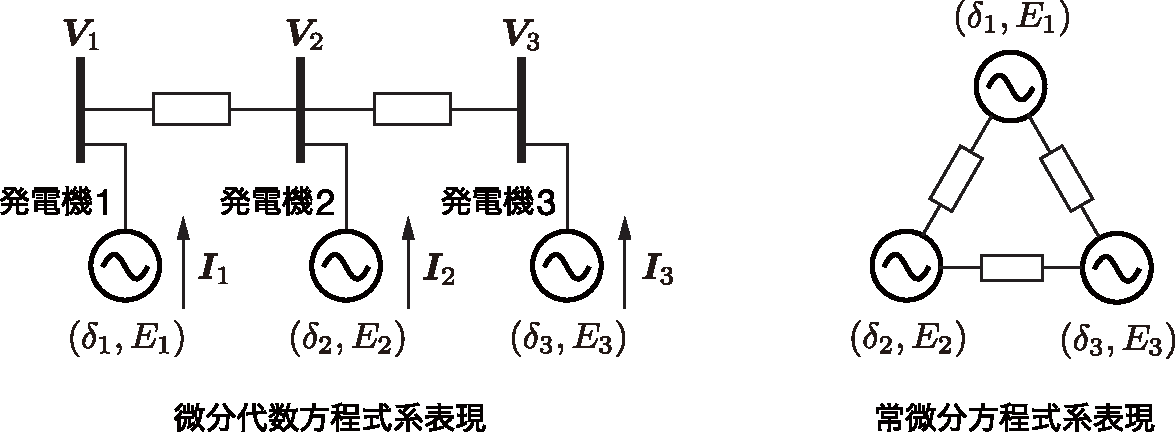
\includegraphics[width = .85\linewidth]{figs/kronredgen}
\medskip
\caption{\textbf{Changes in bond structure due to Kron reduction}}
\label{fig:krongen}
\medskip
\end{figure}


In addition, although the admittance matrix $\bm{Y}$ is a sparse matrix that
reflects the graph structure of the power grid, the reduced admittance matrix
$\bm{Y}^{\rm red}$ in Equation \ref{eq:krondyn} is usually not a sparse matrix.
Therefore, note that the system of ordinary differential equations in Equation
\ref{eq:krondyn} has a coupled structure in which the internal states of all
generators interact closely.  Let's confirm this fact with numerical examples
along with the behavior of the electrical power system model.

\begin{COLUMN}
\noindent \textbf{Sparse and dense matrices}:
A matrix with many 0 elements is called a \textbf{sparse matrix}. In contrast, a
matrix with almost no 0 elements is called a \textbf{dense matrix}. However, how
many 0 elements are necessary to call a matrix sparse matrix depends on the
context. The inverse matrix of a sparse matrix that is not diagonal is usually a
dense matrix.
\end{COLUMN}


\begin{table}[h]
\medskip
 \caption{\textbf{Physical constants of the generator model}}
 \label{table:genparams}
 \centering
  \begin{tabular}{cccccc}
   \hline
$i$ &  $M_i$~[s] & $D_i$~[pu] & $\tau_i$~[s] & $\Xsi$~[pu] & $\Xti$~[pu] \\
   \hline \hline
1 & 100 & 10 & 5.14 & 1.569 & 0.936 \\
   \hline
2 & 18 & 10 & 5.90 & 1.651 & 0.911 \\
   \hline
3 & 12 & 10 & 8.97 & 1.220 & 0.667 \\
   \hline
  \end{tabular}
\end{table}

\begin{table}[h]
\medskip
 \caption{\textbf{Steady-state values of external inputs and internal states of the generator}}
 \label{table:gensteady}
 \centering
  \begin{tabular}{ccccccccccccccccc}
   \hline
$i$ &  $P_{{\rm mech}i}^{\star}$~[pu] & $V_{{\rm filed}i}^{\star}$~[pu] & $\delta_i^{\star}$~[rad] & $\Delta \omega_i^{\star}$~[pu] & $E_i^{\star}$~[pu] \\
   \hline \hline
1 & $-0.5623$ & 1.5132 & 0.4656 & 0 & 1.4363 \\
2 & 0.8832 & 2.2216 & 1.0903 & 0 & 1.8095 \\
3 & $-0.3160$ & 0.9198 & 0.6067 & 0 & 1.1030 \\
   \hline
  \end{tabular}
\end{table}


\begin{example}{\textbf{Behavior of an electrical power system model with a
reduced generator bus}}\label{ex:Kronode}

Let us consider an electrical power system model consisting of three bus bars as
discussed in Example \ref{ex:derY}. Moreover, a synchronous generator is
connected to each bus bar and modeled as the one-axis generator model discussed
in Section \ref{sec:genfund}. Then, the electrical power system model can be
draw as the left picture in Figure \ref{fig:krongen}. The values of the physical
constants of the generators are chosen as in \ref{table:genparams}. Since the
system frequency is set to 60 [Hz], the value of $\omega_0$ is $120\pi$.

The admittance of the two transmission lines is set as:
\begin{equation}\label{eq:defadpara}
  \bm{y}_{12} = 1.3652 - \bm{j} 11.6041, \qquad
  \bm{y}_{23} = 1.9422 - \bm{j} 10.5107
\end{equation}

In this manner, the admittance matrix of the power grid in Equation \ref{eq:exY}
can be obtained. Then, the real and imaginary parts of the reduced admittance
matrix $\bm{Y}^{\rm red}$ can be calculated according to Equation \ref{eq:Yred}.

\begin{equation*}
  \spliteq{
    G^{\rm red}&=
    \mat{
    0.0073  & 0.0005 & -0.0079  \\
    0.0005  & 0.0041 & -0.0046  \\
    -0.0079 & -0.0046 & 0.0125 
    }, \\
    B^{\rm red}&=
    \mat{
    - 0.3716 & - 0.3167 & -0.3800  \\
    - 0.3167 & - 0.3550 & - 0.4260  \\
    - 0.3800 & - 0.4260 & - 0.6933
    }
  }
\end{equation*}

Therefore, both reduced conductance and susceptance matrices are dense. This
dense structure corresponds to the right image of \ref{fig:krongen}.

Next, let us calculate the time response of the ordinary differential equation
system model of Equation \ref{eq:krondyn}. In the following, the initial value
response is obtained when the mechanical power and the magnetic field, which are
external inputs, are fixed to constants.  In this example, we assume that the
steady-state values of the external inputs and internal states of the power
system model are obtained in advance using the steady-state calculation method
that will be described in Section \ref{sec:powerflow}.  Specifically, the input
mechanical power and magnetic field are set to the constant values shown in the
first and second columns of Table \ref{table:gensteady}. In this case, the
steady-state values of the internal states of the power system are given in
columns 3 to 5 of Table \ref{table:gensteady}.

These steady values are one of the solutions that satisfy the following
simultaneous equations:
\begin{equation*}
  \simode{
    0 &= %\textstyle
    - f_i \left( \delta^{\star},E^{\star} \right)
    +P_{{\rm mech}i}^{\star}
    \\
    0 & = %\textstyle
    -  \tfrac{ \Xsi }{\Xti }  E_i^{\star}  + \left(
    \Xsi - \Xti
    \right)
    g_i \left( \delta^{\star},E^{\star} \right)
    + V_{{\rm field}i}^{\star}
  }
  \qquad
  i \in \{1,2,3\}
\end{equation*}
where $\delta^{\star}$ and $E^{\star}$ are vectors composed by
$\delta_i^{\star}$ and $E_i^{\star}$ and the functions $f_i$ and $g_i$ are
defined by Equation \ref{eq:eigidef}.

First, let us consider a situation in which the steady-state value is perturbed
and set as initial value. In other words:

\begin{equation}\label{eq:exdelE0}
  \mat{
    \delta_1(0) \\
    \delta_2(0) \\
    \delta_3(0) 
  }
  =
  \mat{
    \delta_1^{\star} + \tfrac{\pi}{6} \\
    \delta_2^{\star} \\
    \delta_3^{\star} 
  },\qquad
  \mat{
    E_1(0) \\
    E_2(0) \\
    E_3 (0)
  }
  =
  \mat{
    E^{\star}_1 +0.1 \\
    E^{\star}_2 \\
    E^{\star}_3 
  }
\end{equation}
where the initial value of the frequency deviation is 0. Then, the time response of
the electrical power system model is shown in \ref{fig:Kron0}.

From this figure, it can be seen that after the angular frequency deviation and
rotor deflection angle oscillate for about 15 seconds, they asymptotically
converge to the original steady state. However, since the behavior of the rotor
angle is only affected by the relative difference among generators, the
convergence value of the rotor angle is shifted from the original steady state
value by a constant. In other words, for a certain constant $c_0$:

\[
  \lim_{t\rightarrow \infty} \delta_i(t) = \delta_i^{\star} +c_0,\qquad
  \forall i \in \{1,2,3\}
\]

For any value of $c_0$, the steady value is essentially equivalent. The voltage
phasor of the bus bar shown in Figure \ref{fig:Kron0} can be calculated
independently of the internal state of the generators by using the Equation
\ref{eq:colVi}. Similarly, the active and reactive power can be calculated
independently using Equation \ref{eq:PiQis2}. Furthermore, since the frequency
deviation is equal to $5\times 10^{-3}$~[pu] times the system frequency, it is
equal to 0.3 [Hz]. 

Next, let us consider a case where the value of an external input is perturbed.
Specifically, let us consider a perturbation in the mechanical power of
generator 1.

\[
  \mat{
    P_{{\rm mech}1}(t) \\
    P_{{\rm mech}2}(t) \\
    P_{{\rm mech}3}(t) 
  }=
  \mat{
    P_{{\rm mech}1}^{\star} +0.05\\
    P_{{\rm mech}2}^{\star} \\
    P_{{\rm mech}3}^{\star} 
  }
\]

Figure \ref{fig:KronP} shows the time response of the electrical power system
model under this condition. The initial value is set to be the same as in
Equation \ref{eq:exdelE0}. In addition, the phase of the rotor angle and the bus
voltage phasor are the remainder of the division by $\pi$. In this case, it can
be seen that the angular frequency deviation does not become 0 in the steady
state, and the integral of the rotor angle changes constantly.  Figure
\ref{fig:KronV} shows the time response of the electrical power system model
when field voltage of generator 1 is similarly perturbed:

\[
  \mat{
    V_{{\rm filed}1}(t) \\
    V_{{\rm filed}2}(t) \\
    V_{{\rm filed}3}(t) 
  }=
  \mat{
    V_{{\rm filed}1}^{\star} +0.5 \\
    V_{{\rm filed}2}^{\star} \\
    V_{{\rm filed}3}^{\star} 
  }
\]

Similarly, in this situation the frequency deviation in a steady state does not
become 0. Therefore, to calculate the time response of an electrical power
system model, not only the initial values, but also the external inputs, such as
mechanical power and field voltage, must be set to appropriate values.
\end{example}


Since Equation \ref{eq:krondyn} is an ordinary differential equation system
model, it is possible to numerically simulate its behavior by using differential
equation solvers in MATLAB. However, as shown in Example \ref{ex:Kronode},
unless the value of the mechanical power and the field voltage are set
appropriately, the frequency deviation of each generator does not converge to 0
in the steady state, and the rotor argument constantly deviates from the
reference. Thus, to perform a numerical simulation that is realistically
meaningful, a method to calculate valid equilibrium points and initial values is
necessary. These details will be explained in Chapter \ref{chap:numcal}.

\begin{figure}[t]
  \centering
  {
  \begin{minipage}{0.49\linewidth}
    \centering
    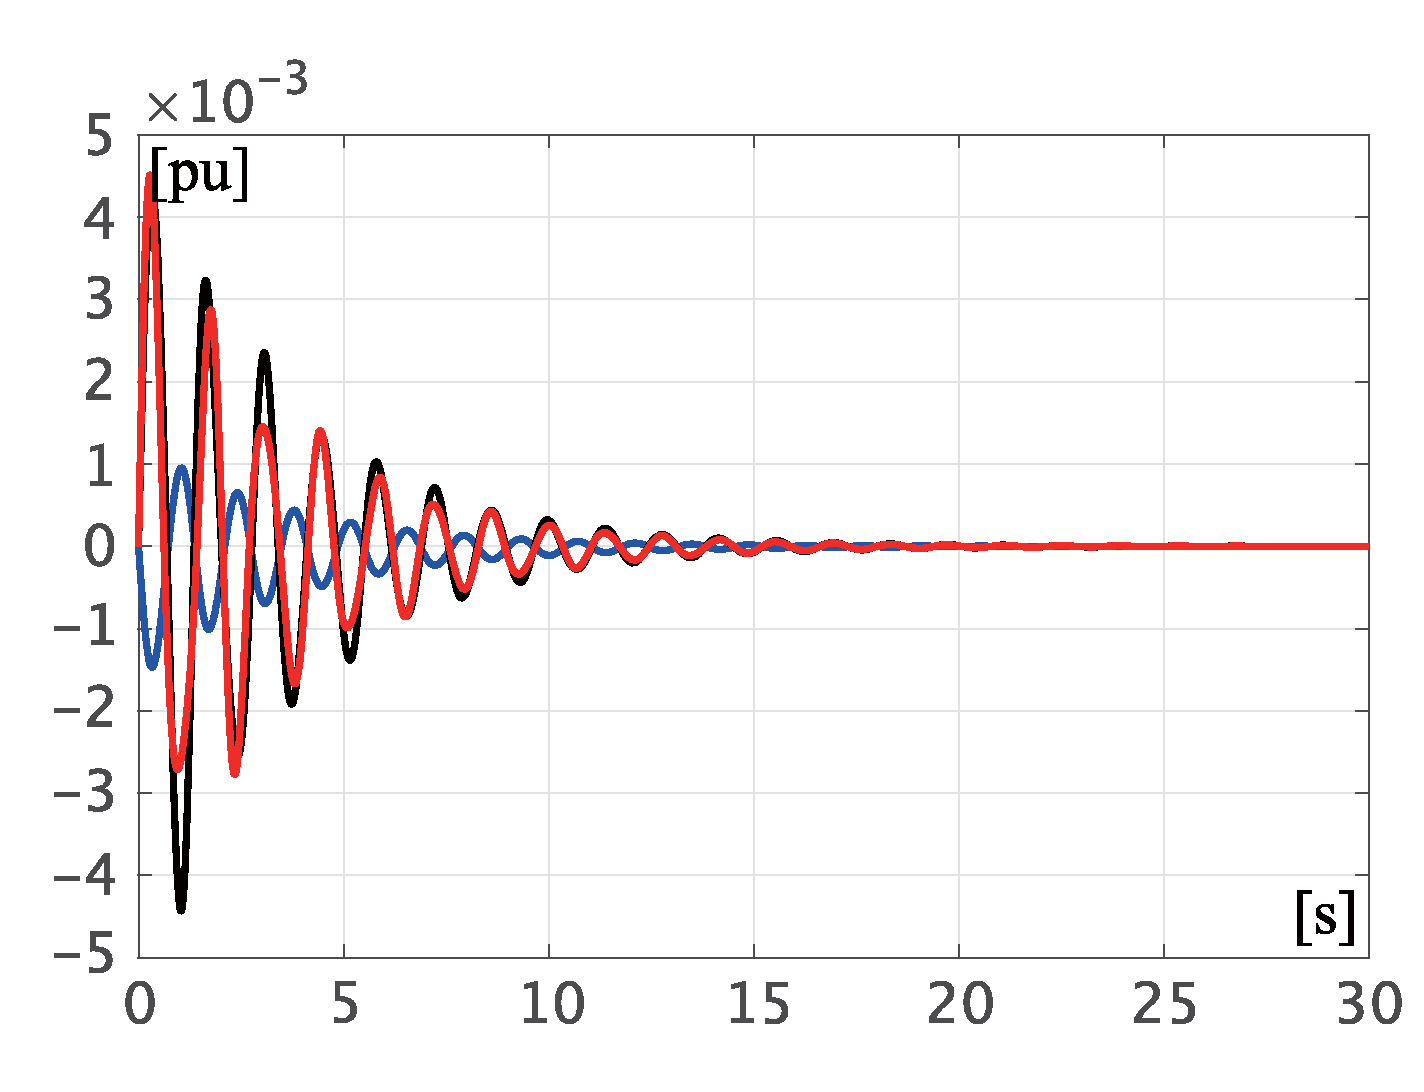
\includegraphics[width = 1.0\linewidth]{figs/Domega0}
    \subcaption{ $\Delta \omega_i$}
    \medskip
  \end{minipage}
  \begin{minipage}{0.49\linewidth}
    \centering
    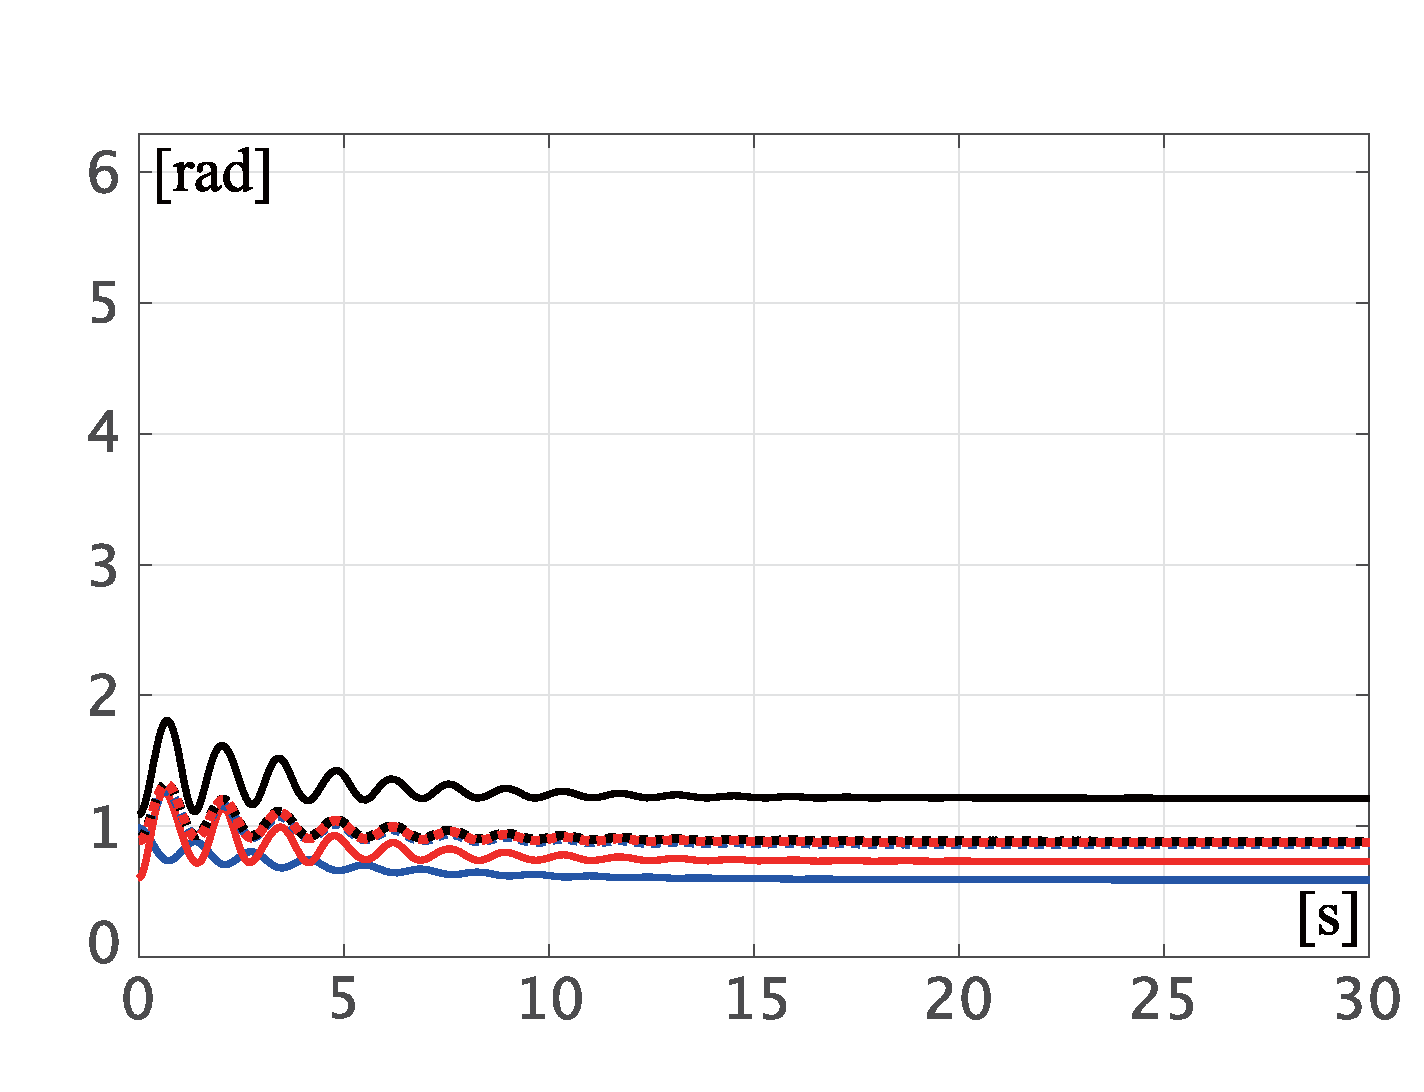
\includegraphics[width = 1.0\linewidth]{figs/delangV0}
    \subcaption{ Solid line: (1)$\delta_i$, Dashed line: $\angle \bm{V}_i$ }
    \medskip
  \end{minipage}
 \begin{minipage}{0.49\linewidth}
    \centering
    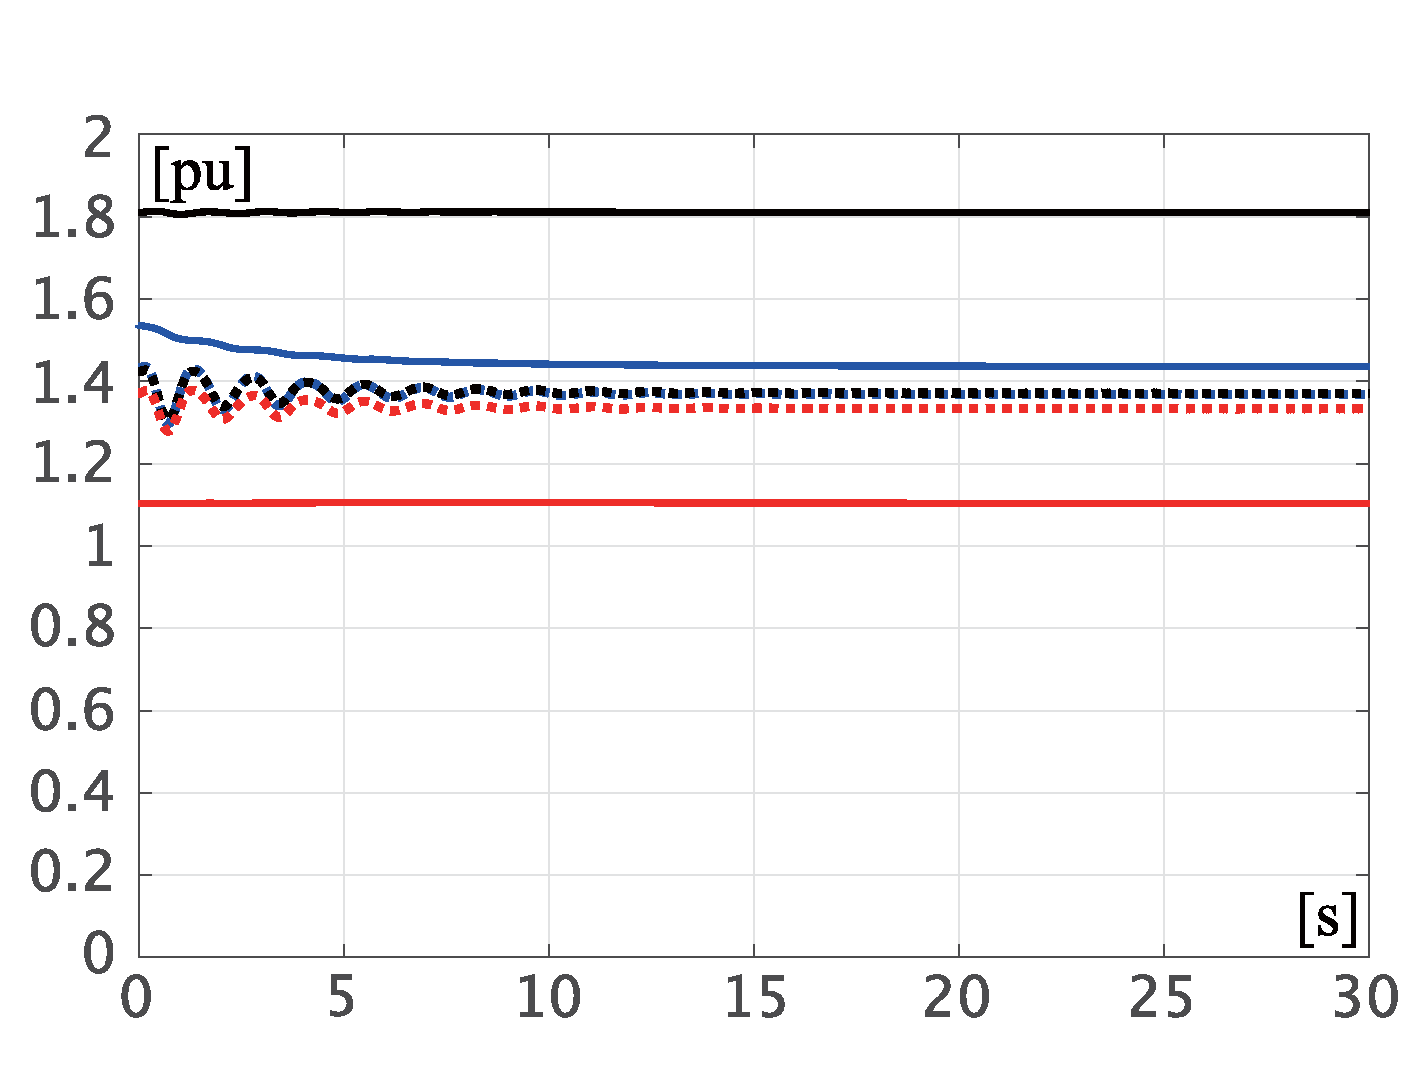
\includegraphics[width = 1.0\linewidth]{figs/EabsV0}
    \subcaption{ Solid line: $E_i$, Dashed line: $|\bm{V}_i|$ }
    \medskip
  \end{minipage}
  \begin{minipage}{0.49\linewidth}
    \centering
    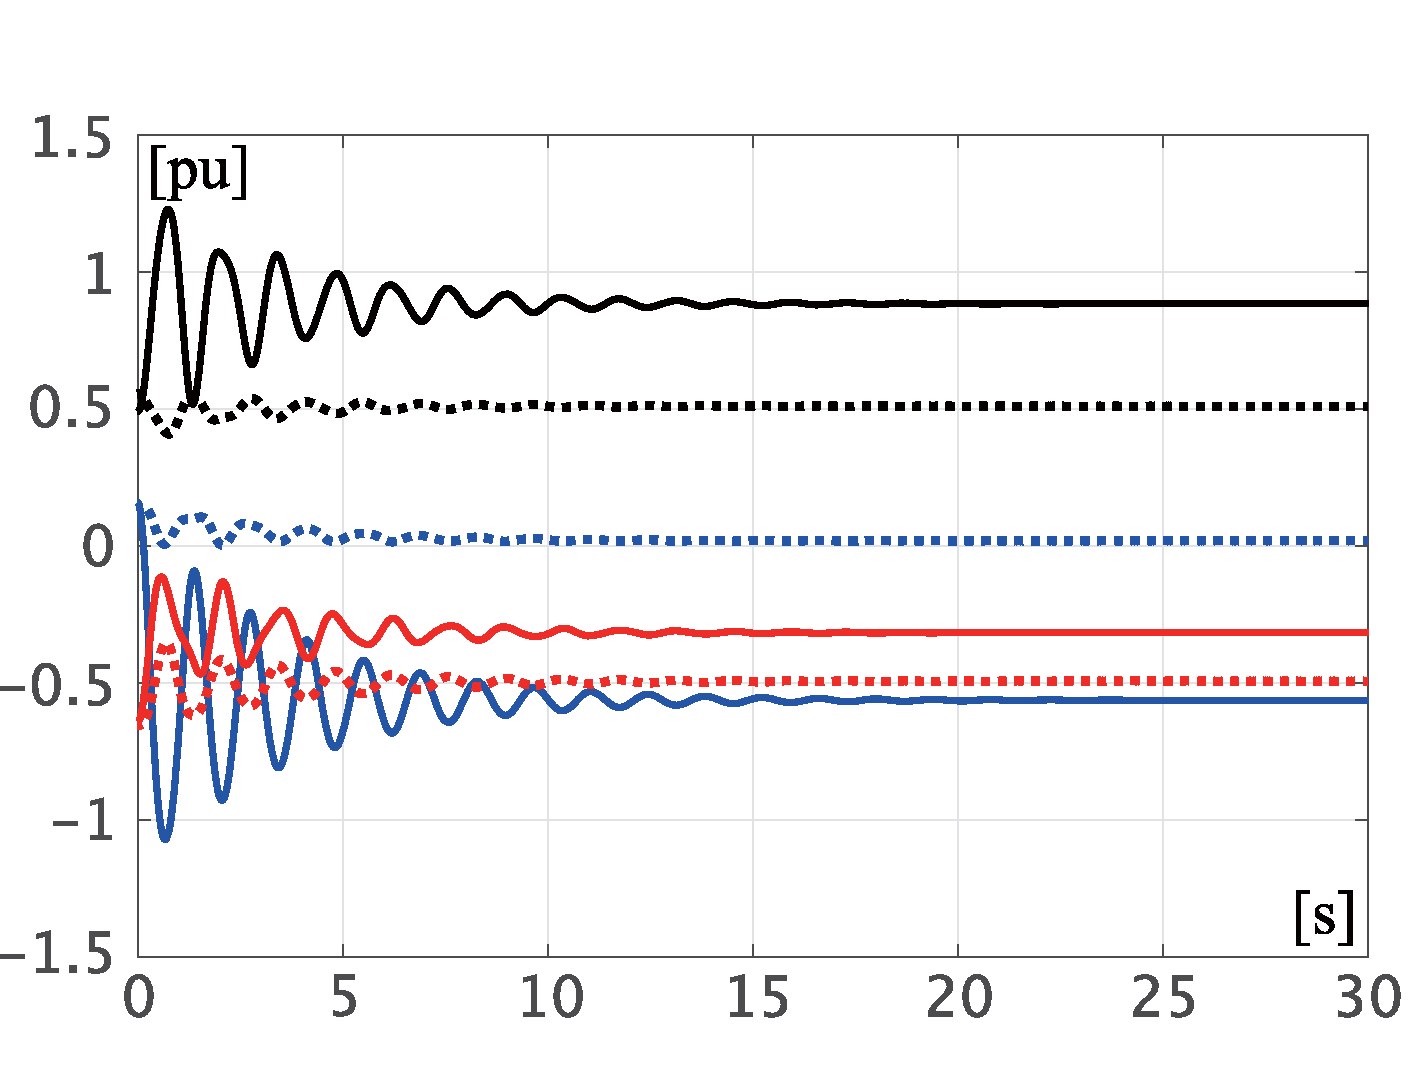
\includegraphics[width = 1.0\linewidth]{figs/PQ0}
    \subcaption{ Solid line: $P_i$, Dashed line: $Q_i$ }
    \medskip
  \end{minipage}
  }
  \medskip
  \caption{\textbf{System time response for perturbated initial value}
  \\  \centering((Blue: Bus 1, Black: Bus 2, Red: Bus 3))}
  \label{fig:Kron0}
\medskip
\end{figure}

\begin{figure}[t]
  \centering
  {
  \begin{minipage}{0.49\linewidth}
    \centering
    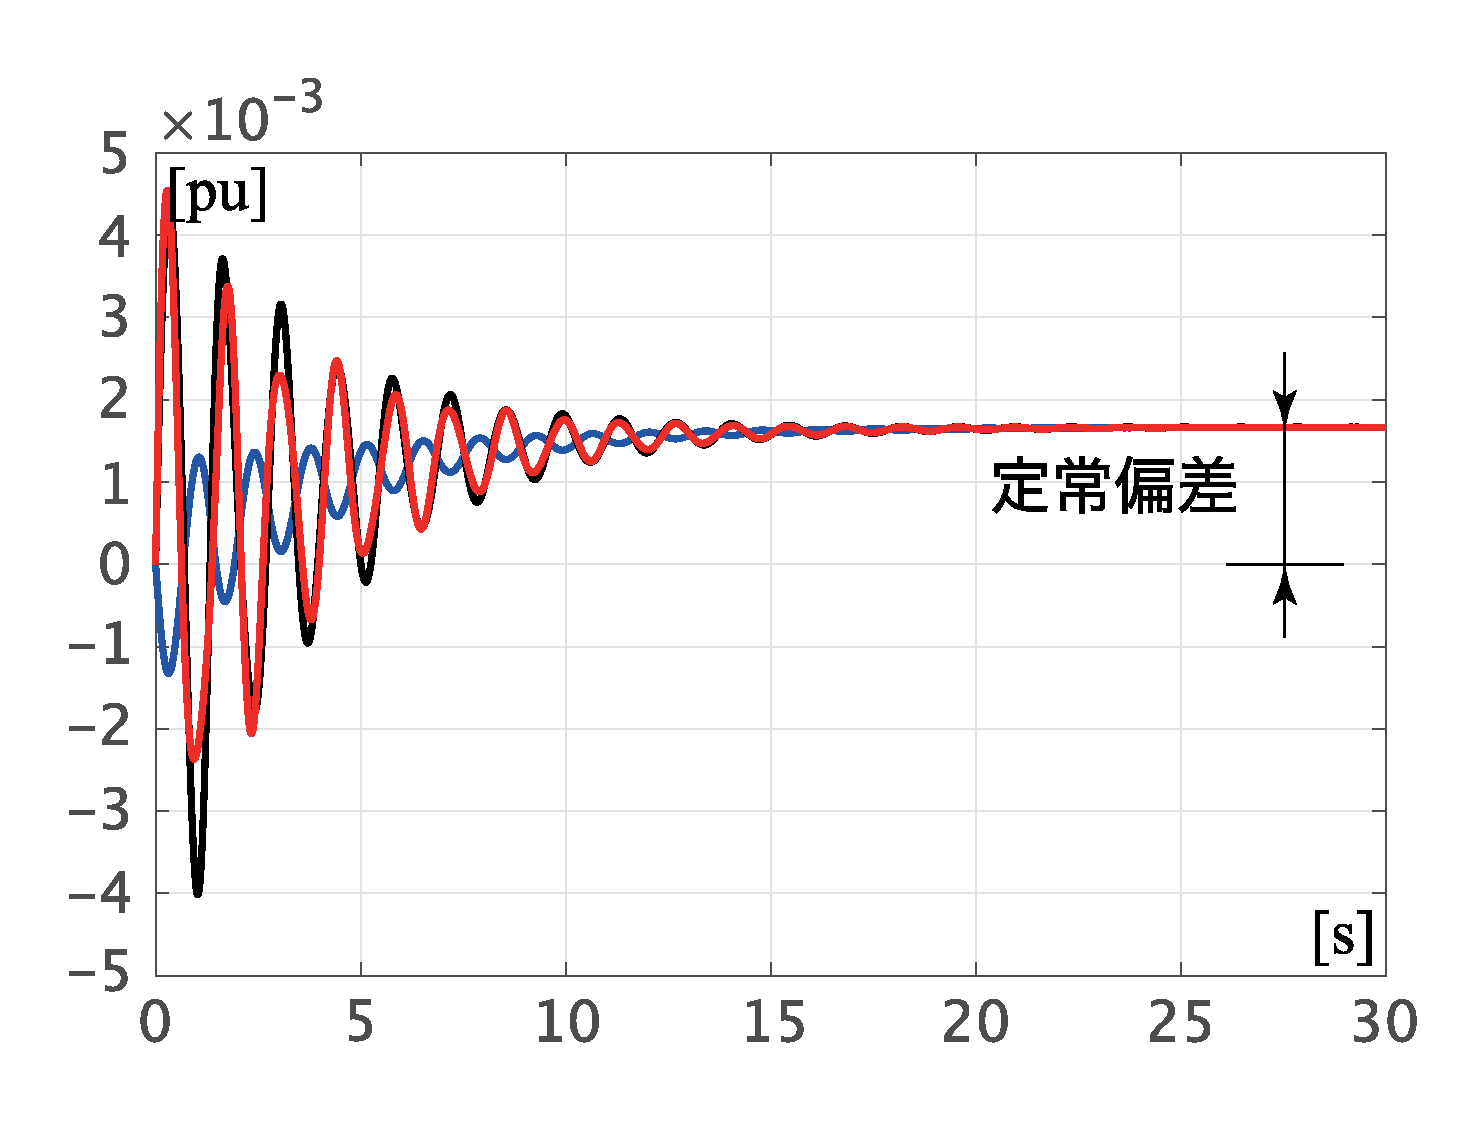
\includegraphics[width = 1.0\linewidth]{figs/DomegaP}
    \subcaption{ $\Delta \omega_i$ }
    \medskip
  \end{minipage}
  \begin{minipage}{0.49\linewidth}
    \centering
    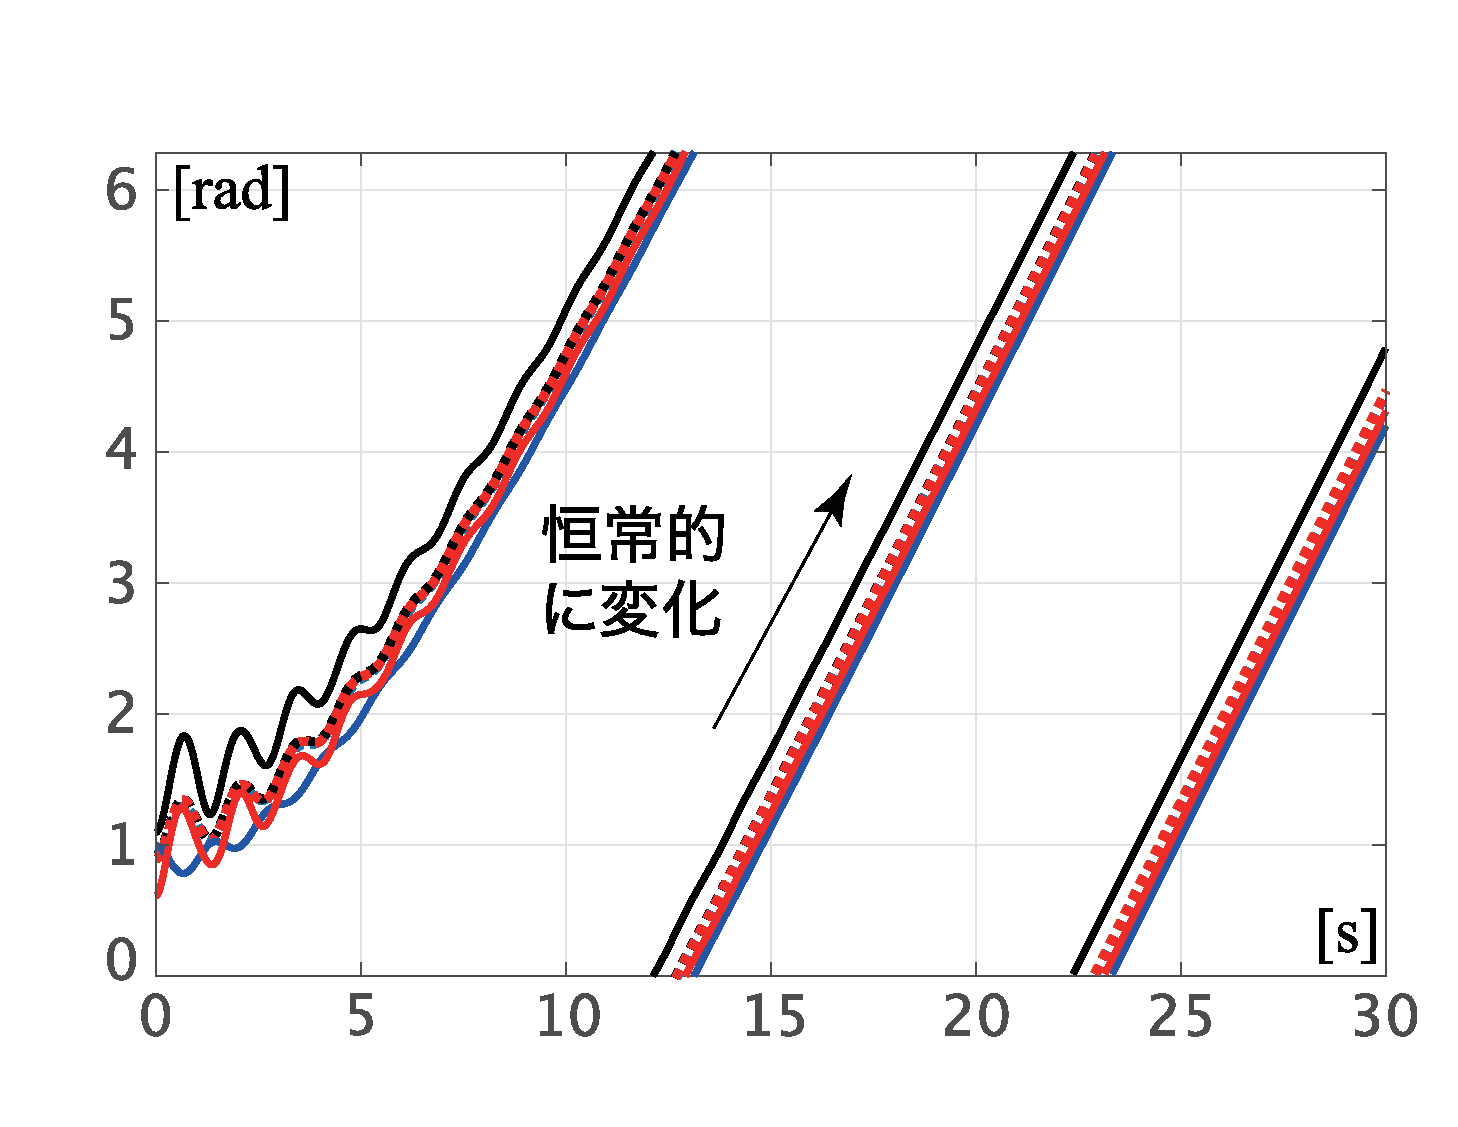
\includegraphics[width = 1.0\linewidth]{figs/delangVP}
    \subcaption{ Solid line: $\delta_i$, Dashed line:$\angle \bm{V}_i$ }
    \medskip
  \end{minipage}
 \begin{minipage}{0.49\linewidth}
    \centering
    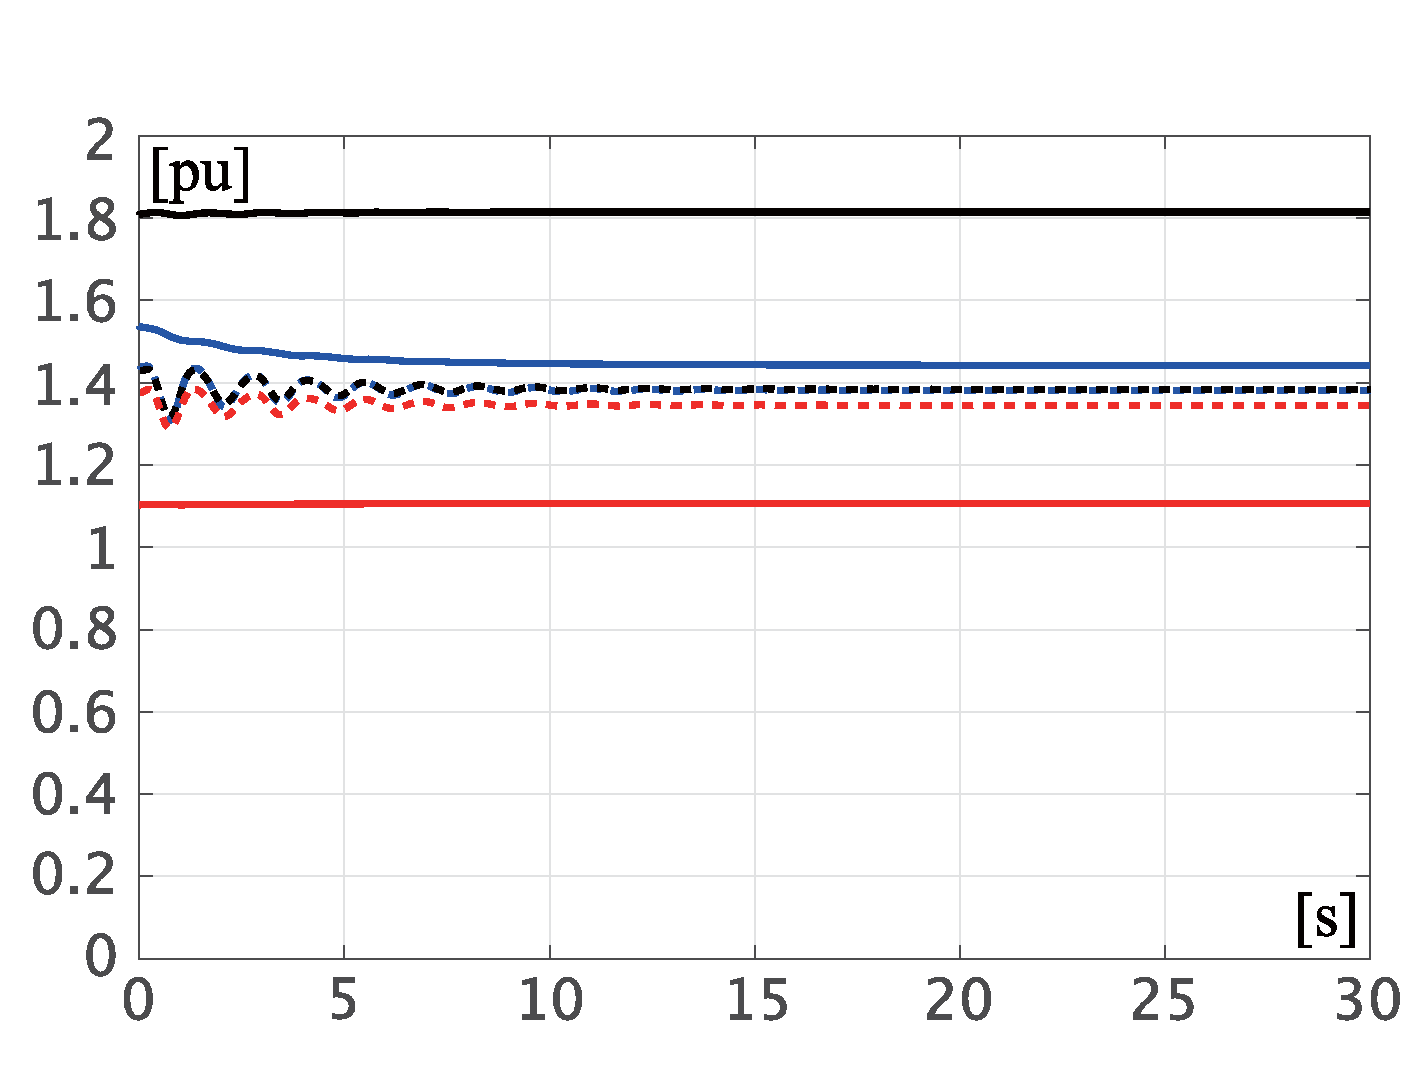
\includegraphics[width = 1.0\linewidth]{figs/EabsVP}
    \subcaption{ Solid line: $E_i$, Dashed line:$|\bm{V}_i|$ }
    \medskip
  \end{minipage}
  \begin{minipage}{0.49\linewidth}
    \centering
    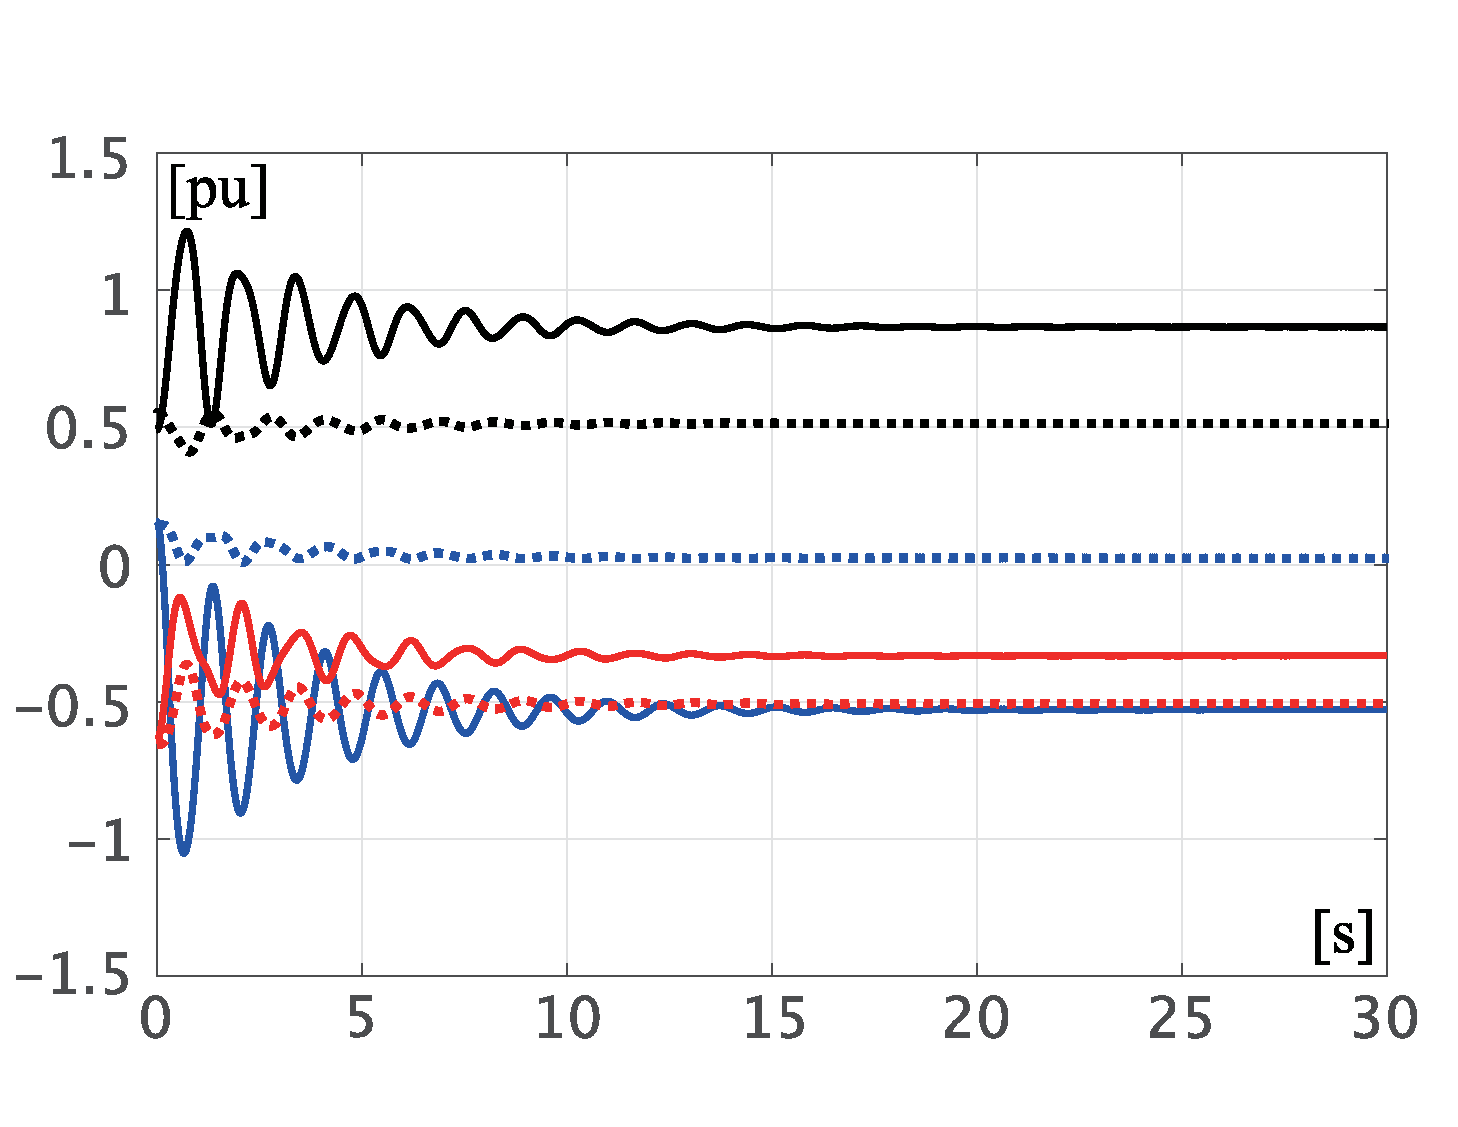
\includegraphics[width = 1.0\linewidth]{figs/PQP}
    \subcaption{ Solid line: $P_i$, Dashed line:$Q_i$ }
    \medskip
  \end{minipage}
  }
  \medskip
  \caption{\textbf{System time response when perturbation is applied to the mechanical power}
  \\  \centering(Blue: Bus 1, Black: Bus 2, Red: Bus 3)}
  \label{fig:KronP}
\medskip
\end{figure}

\begin{figure}[t]
  \centering
  {
  \begin{minipage}{0.49\linewidth}
    \centering
    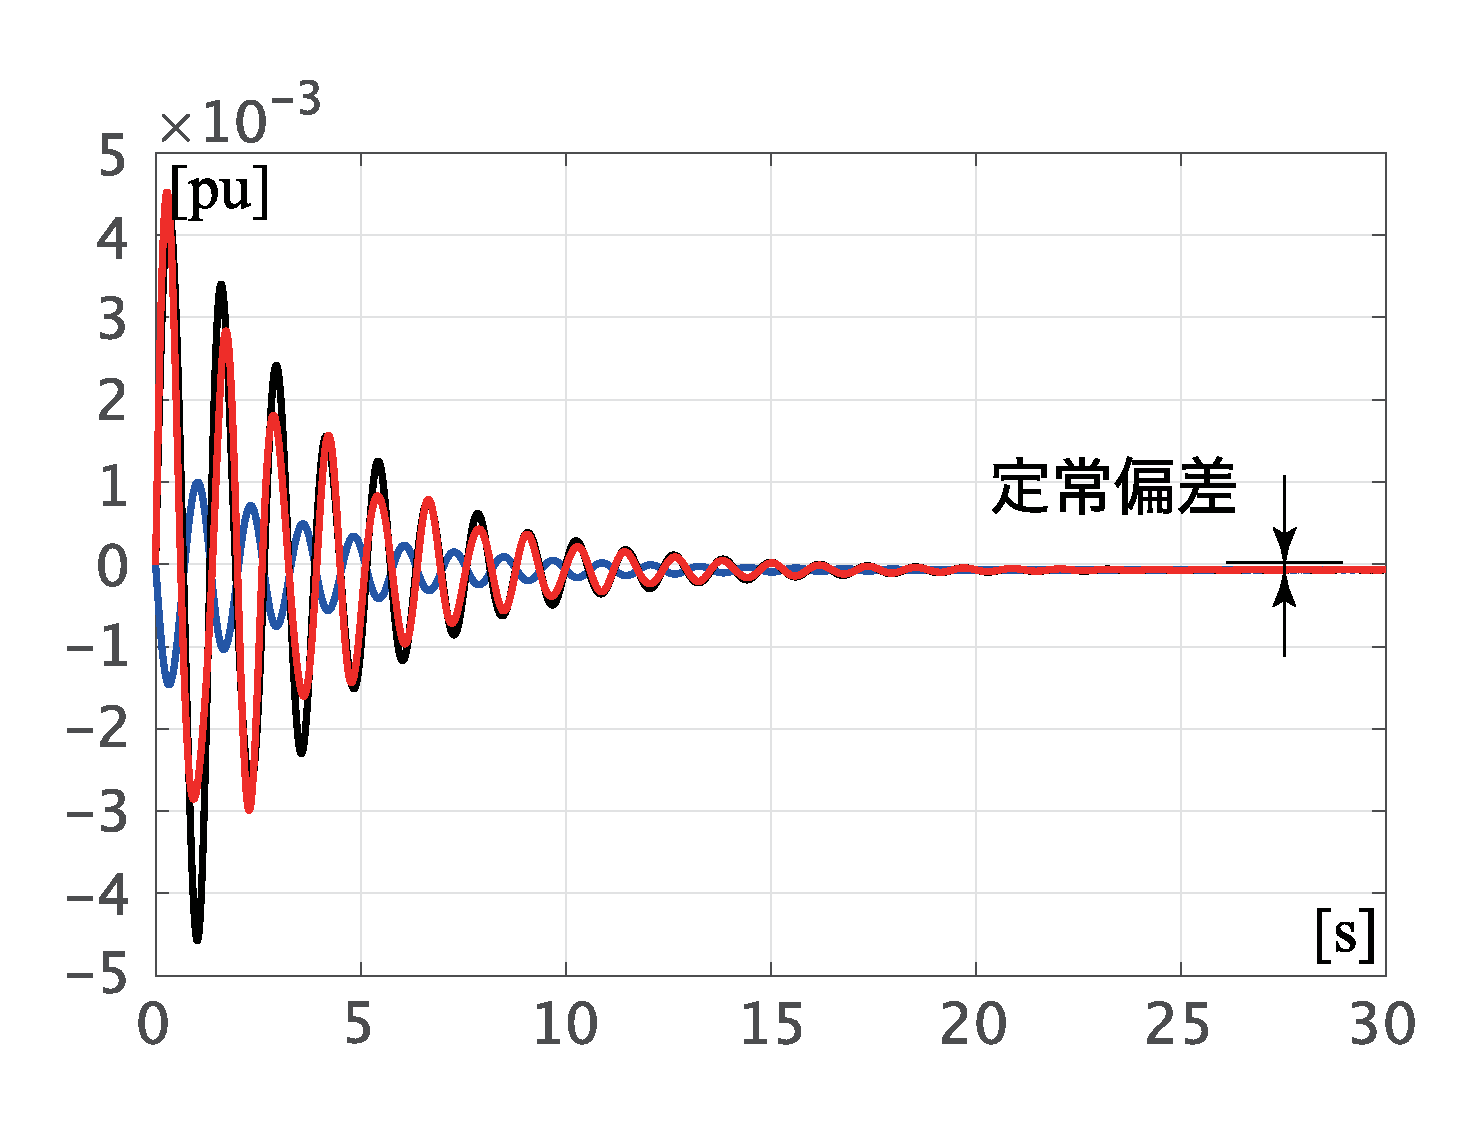
\includegraphics[width = 1.0\linewidth]{figs/DomegaV}
    \subcaption{ $\Delta \omega_i$ }
    \medskip
  \end{minipage}
  \begin{minipage}{0.49\linewidth}
    \centering
    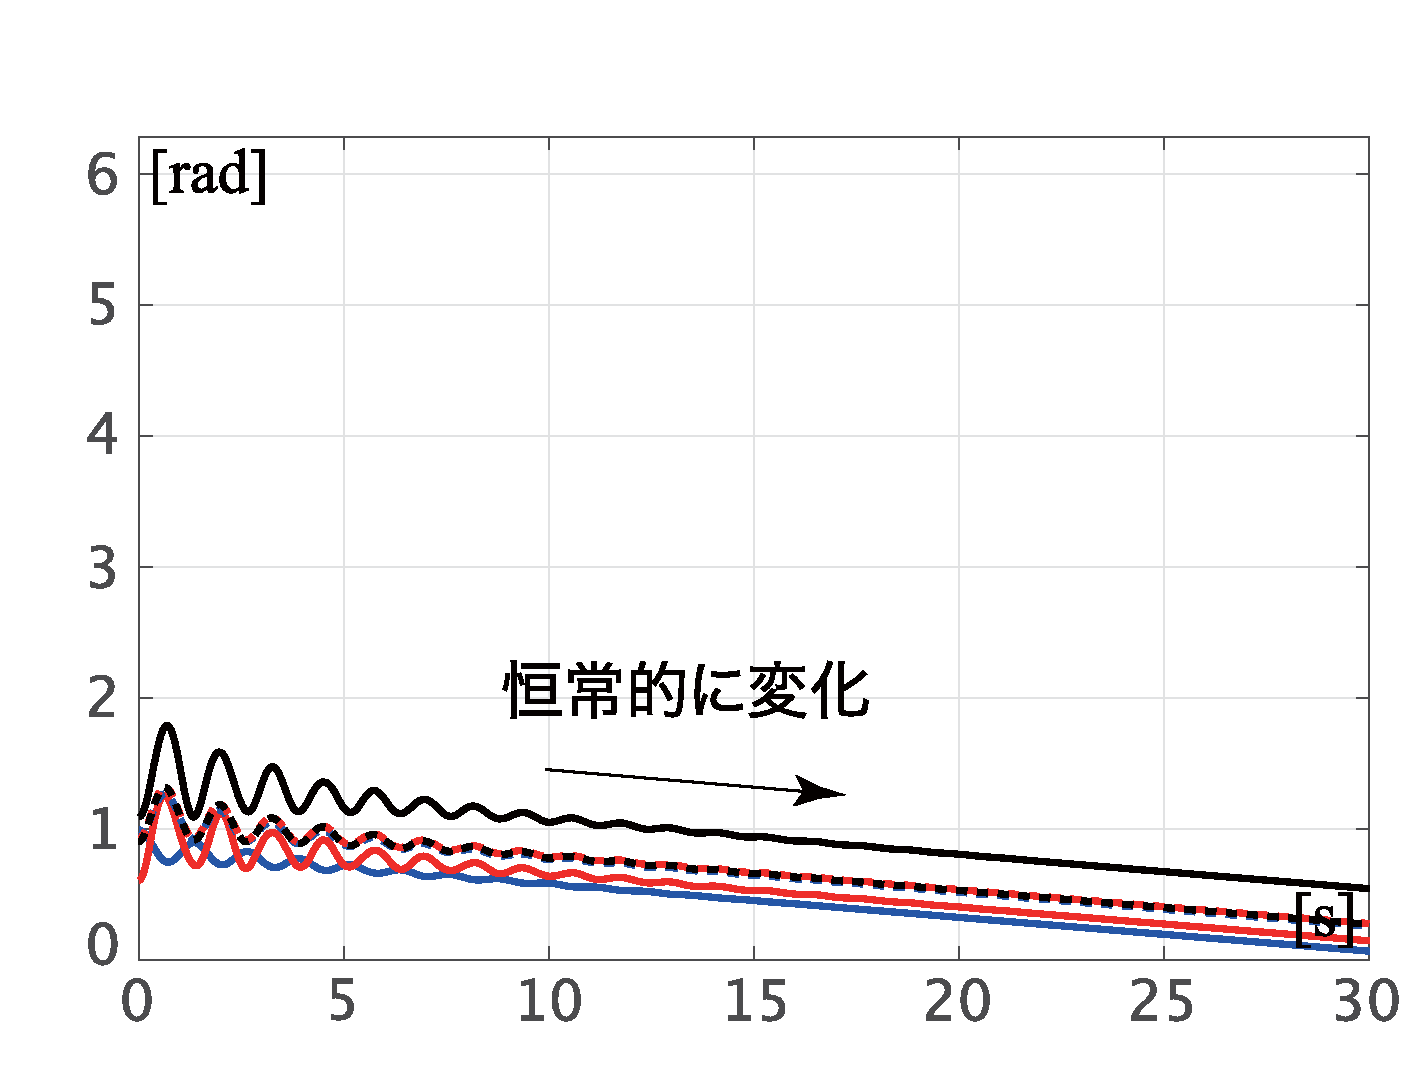
\includegraphics[width = 1.0\linewidth]{figs/delangVV}
    \subcaption{ Solid line: $\delta_i$, Dashed line:$\angle \bm{V}_i$ }
    \medskip
  \end{minipage}
 \begin{minipage}{0.49\linewidth}
    \centering
    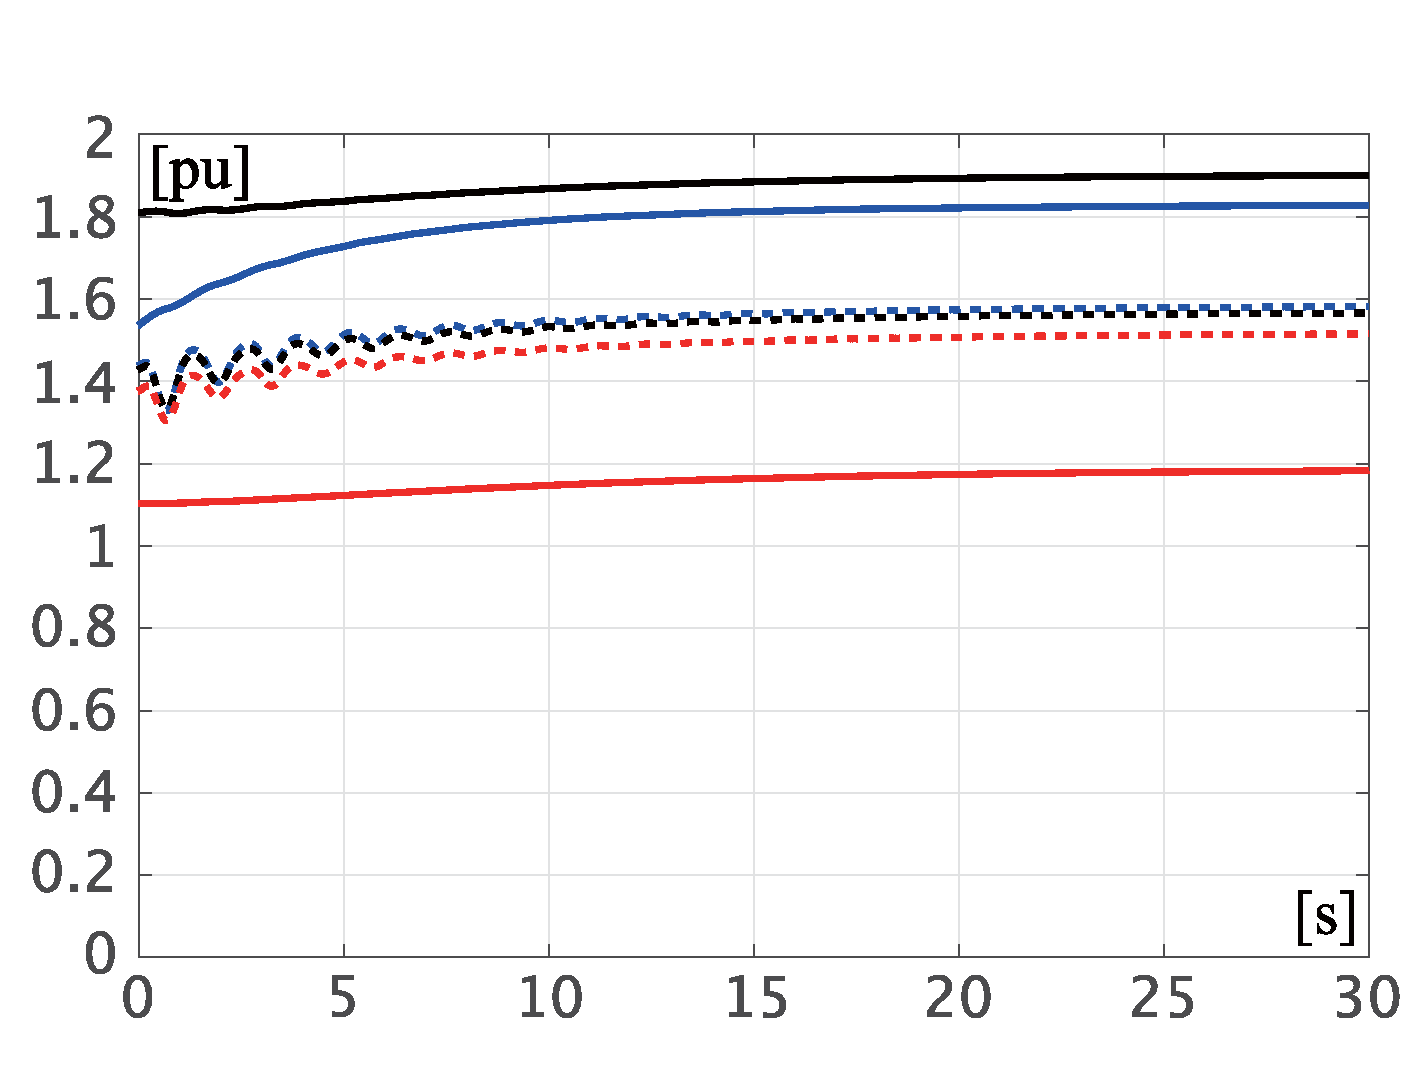
\includegraphics[width = 1.0\linewidth]{figs/EabsVV}
    \subcaption{ Solid line: $E_i$, Dashed line:$|\bm{V}_i|$ }
    \medskip
  \end{minipage}
  \begin{minipage}{0.49\linewidth}
    \centering
    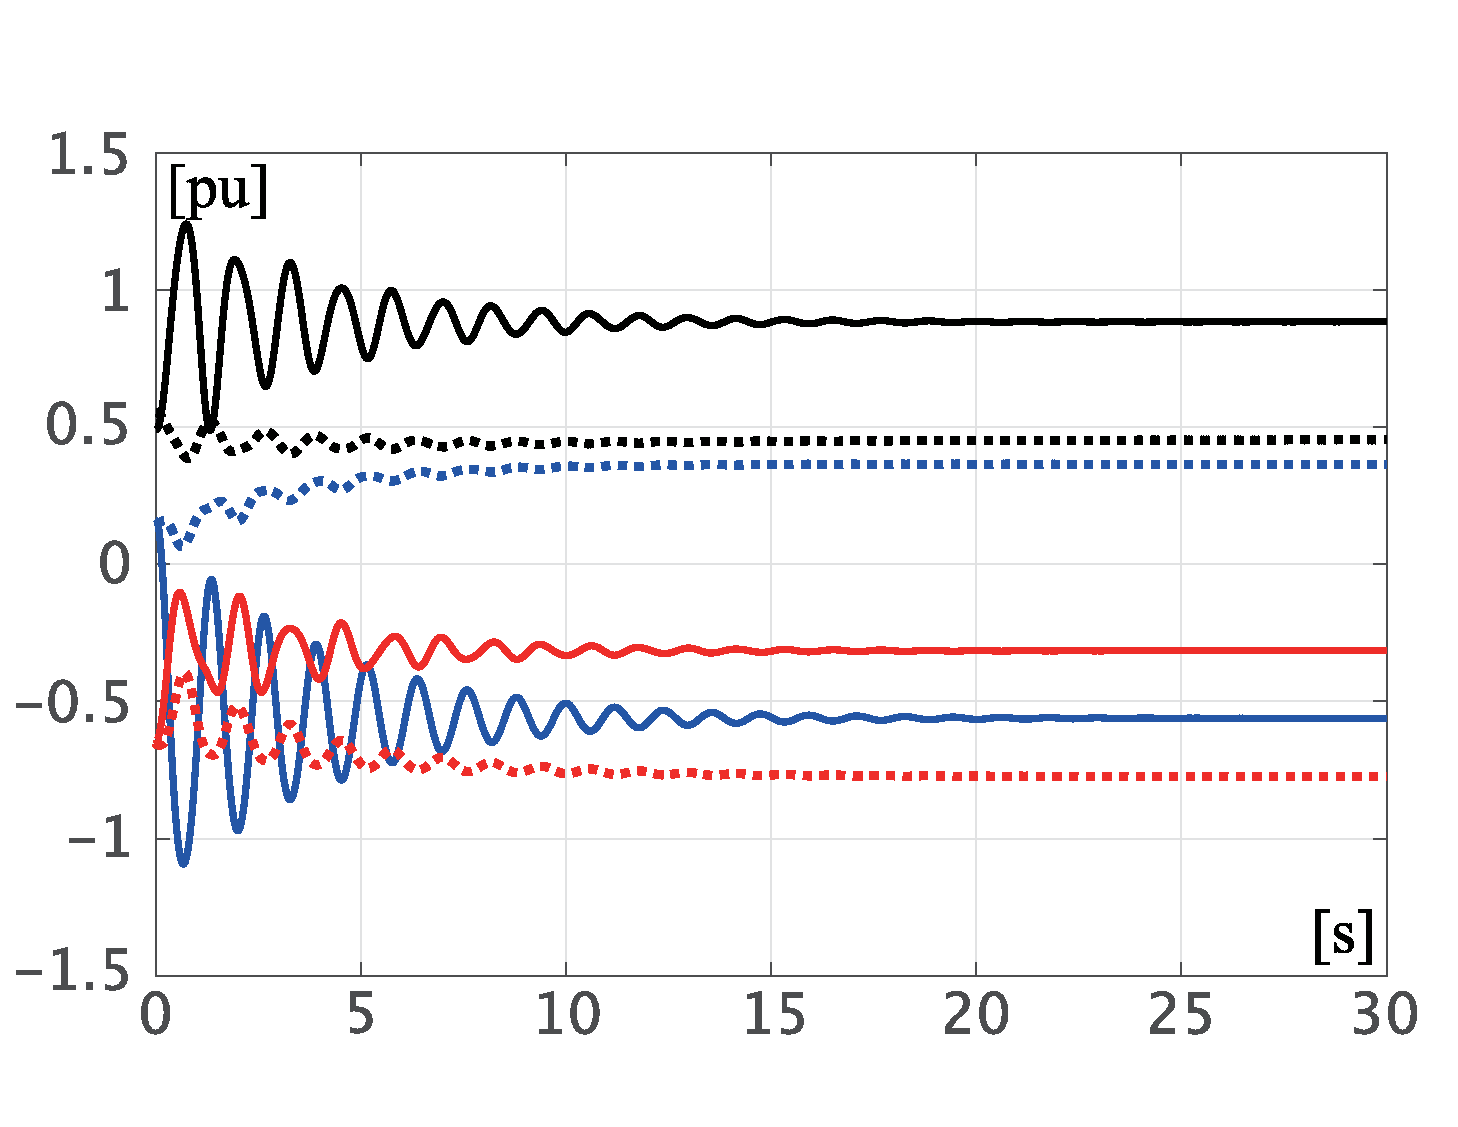
\includegraphics[width = 1.0\linewidth]{figs/PQV}
    \subcaption{ Solid line: $P_i$, Dashed line:$Q_i$ }
    \medskip
  \end{minipage}
  }
  \medskip
  \caption{\textbf{System time response when perturbation is applied to the field voltage}
  \\  \centering(Blue: Bus 1, Black: Bus 2, Red: Bus 3)}
  \label{fig:KronV}
\medskip
\end{figure}

\subsection{Derivation of the Kuramoto-type oscillator model}\label{sec:kuramod}

By applying Kron reduction of generator bus to the classical model explained in
Section \ref{sec:genfund}, a Kuramoto-type oscillator model can be derived.

Specifically, if we assume that the value of synchronous and transient
reactances, $\Xsi$ and $\Xti$, are equal, and that the field voltage $V_{{\rm
field}i}$ is constant and equal to $V_i^{\star}$, the internal voltage $E_i$ is
constant and equal to $V_i^{\star}$. Therefore, the model of an electrical power
system with synchronous generators connected to each bus bar is expressed by the
following ordinary differential equation.

\begin{equation}\label{eq:clamod}
  \simode{
    \dot{\delta}_i&= \omega_0  \Delta \omega_i\\
    M_i   \Delta \dot{\omega}_i&= 
    - D_i \Delta\omega_i - 
    \hat{f}_i (\delta)
    +P_{{\rm mech}i} 
  }\qquad
  i\in \mathcal{I}_{\rm G}
\end{equation}

However, the nonlinear term is given by:

\[
  \hat{f}_i (\delta):=
  - V_i^{\star} \sum_{j=1}^{N}
  V_j^{\star}\left(
  B_{ij}^{\rm red}   \sfsin \delta_{ij}
  -
  G_{ij}^{\rm red}   \sfcos \delta_{ij}
  \right)
\]

The function $\hat{f}_i (\delta)$ expresses the active power of a generator $i$.
An electrical power system mode whose transmission lines have zero conductance,
that is $G_{ij}^{\rm red}=0$, is occasionally used.


\begin{COLUMN}

\noindent\textbf{Kuramoto model}:

The following differential equation system comprising of $N$ oscillators moving
on the circumference is called \textbf{Kuramoto model}.

\[
  \dot{\theta}_i = \omega_i - \frac{K}{N} \sum_{j=1}^N \sfsin (\theta_i - \theta_j),
  \qquad
  i=1,\ldots,N
\]

In this context, $\omega_i$ is a constant representing the intrinsic angular
velocity of the oscillator $i$, and $K$ is a constant representing the coupling
strength. In general, when the coupling strength $K$ is sufficiently large
compared to the magnitude of the inhomogeneity of the intrinsic angular speeds
$\omega_1,\ldots,\omega_N$, the angular speeds of the oscillator,
$\dot{\theta}_1,\ldots,\dot{\theta}_N$, are asymptotically synchronized.

The Kuramoto model has been analyzed mainly in the field of physics as a
mathematical model describing the synchronization phenomena of nonlinear
oscillators, and is known to have a wide range of applications
\cite{kuramoto1975self,kuramoto2003chemical}. The nonlinear second-order
oscillator model with inertial is also applied to the analysis of
synchronization in power systems
\cite{dorfler2012synchronization,dorfler2013synchronization,nagata2014node,nishikawa2015comparative}.
\end{COLUMN}

\subsection{Single machine infinite bus system model}\label{sec:onemachine}

\begin{figure}[t]
\centering
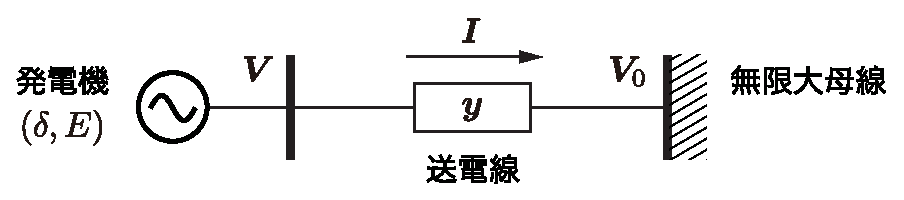
\includegraphics[width = .70\linewidth]{figs/inf1bus}
\medskip
\caption{\textbf{Single machine infinity bus system model}}
\label{fig:inf1bus}
\medskip
\end{figure}

The \textbf{single machine infinite bus system model} is a simplified electrical
power system model that is often used in basic mathematical analysis of
electrical power systems, such as in \cite[Section 1.3]{taniguchi2011power} and
\cite[Section 6.3, Section 8.3]{kato2017electric}. It is an electrical power
system model consisting of a generator, a transmission line, and an infinite bus
bar as shown in Figure \ref{fig:inf1bus}. The infinite bus bar is interpreted as
a rough approximation of the entire electrical power system, except for the
generator of interest, as a "fixed voltage source".

Specifically, we assume that voltage phasor of the infinite bus bar $\bm{V}_0$
is maintained as constant regardless the internal state of the generator.  In
other words, considering a transmission loss of electric power, the active and
reactive power generated by the generator are assumed to be consumed each
moment, without excess or deficiency, by the infinite bus bar.

In the following, we only focus on one generator, so we omit the subscript $i$
and denote the variables of the generator and the generator bus. For the dynamic
characteristics of the generator expressed in Equation (\ref{eq:gendynVI}), the
voltage phasor $\bm{V}$ and current phasor $\bm{I}$ of a generator bus have the
following relationship:

\[
  \bm{I}= \bm{y} (\bm{V}-\bm{V}_0)
\]

This is an algebraic equation that determines the input-output relationship of
the generator and the electrical power system. For reference, let us derive an
ordinary differential equation model from the Kron reduction of the single
machinen infinite bus bar system when the resistance of the transmission line is
0 and the reactance $x$. In other words, the admittance of the transmission line
is:

\[
  \bm{y} = \frac{1}{\bm{j} x}
\]

Specifically, following the same procedure as of the Kron reduction of a
generator bus in Section \ref{sec:allgen}, the following two equations are used
to replace the current and voltage phasors of the generator bus.

\[
  \bm{I}= \frac{1}{\bm{j} x} (\bm{V}-\bm{V}_0)
  ,\qquad
  \bm{I}= \frac{1}{\bm{j} \Xt} (Ee^{\bm{j}\delta} -\bm{V})
\]

By substituting the voltage phasor and reorganizing the equation, the following
is obtained:

\[
  |\bm{I}| e^{\bm{j}(\delta -\angle \bm{I})}
  =
  -\frac{
  E- |\bm{V}_0|e^{\bm{j}\delta}
  }{
  \bm{j}(\Xt + x )
  }
\]

However, without loss of generality, $\angle \bm{V} = 0$ with respect to the
phase of the infinite bus voltage phasor. Therefore, by replacing the current
phasor into Equation \ref{eq:gendynIVst}, the expression of the ordinary
differential equation system is obtained as follows:

\begin{equation*}%\label{eq:gendynIVst}
  \simode{
    \dot{\delta} &= \omega_0  \Delta \omega\\
    M   \Delta \dot{\omega}&= \textstyle
    - D \Delta\omega  - 
    \tfrac{
    E|\bm{V}_0|
    }{
    \Xt + x
    }
    \sfsin\delta
    +P_{{\rm mech}}
    \\
    \taud \dot{E} & = \textstyle
    - 
    \tfrac{
    \Xs + x
    }{
    \Xt + x
    }
    E
    +
    \tfrac{
    \Xs - \Xt
    }{
    \Xt + x
    }
    |\bm{V}_0| \sfcos\delta
    + V_{{\rm field}}
  }
\end{equation*}

Similarly, from Equation \ref{eq:PiQis2} the active and reactive power supplied
from the generator to the bus bar can be calculated as follows:

\[
  P=\frac{
  E|\bm{V}_0|\sfsin\delta
  }{
  \Xt + x
  }
  ,\qquad
  Q=
  \frac{
  x E^2 + (\Xt - x )E|\bm{V}_0|\sfcos\delta
  - \Xt |\bm{V}_0|^2
  }{
  ( \Xt + x )^2
  }
\]

In practice, since electrical power systems consist of multiple generators, the 
single machine infinite bus system model is not usually used in this book. The
introduction of this model only serves as a reference.

\subsection{Mathematical properties of the admittance matrix with reduced
generator bus}

Below, we mathematically discuss the existence and definiteness of the reduced
admittance matrix $\bm{Y}^{\rm red}$ of Equation \ref{eq:Yred}. Let us remember
that when the capacitance to ground can be ignored, the conductance matrix $G_0$
is positive semi-definite and the susceptance matrix $B_0$ is negative definite.
Moreover, the reduced conductance and susceptance matrices, which correspond to the
real and imaginary parts of $\bm{Y}^{\rm red}$ are expressed as follows:

\begin{equation}\label{eq:GredBred}
  G^{\rm red} :=\operatorname{Re}\bigl[\bm{Y}^{\rm red}\bigr] ,\qquad
  B^{\rm red} :=\operatorname{Im}\bigl[\bm{Y}^{\rm red}\bigr] 
\end{equation}

Then, the following facts hold.

\begin{theorem}[Existence and definiteness of the reduced admittance matrix]
\label{thm:redadmat}

If the following is true for the admittance matrix $\bm{Y}\in
\mathbb{C}^{N\times N}$ of Equation \ref{eq:Ypig}:

\begin{equation}\label{eq:Xbeta}
  \Cgi \Xti \leq 1
  ,\qquad \forall i \in \mathcal{I}_G
\end{equation}

and at the same time for at least one generator bus the inequality in Equation
\ref{eq:Xbeta} is strict, then  $\bm{\itGamma}$ of Equation \ref{eq:defGam} is
nonsingular. Moreover, for the admittance matrix $\bm{Y}^{\rm red}$ of Equation
\ref{eq:Yred}, the reduced conductance matrix $G^{\rm red}$ is positive
semi-definite, and the reduced susceptance matrix $B^{\rm red}$ is negative
definite.
\end{theorem}

\begin{proof}
By using the Mathematical Supplement \ref{lem:nonsing} at the end of this
chapter, we prove the singularity of $\bm{\itGamma}$ of Equation
\ref{eq:defGam}. From the definition, if $M$ and $N$ are the real and imaginary parts of 
$\bm{\itGamma}$, respectively, then:

\begin{equation*}
  \spliteq{
    M &:= \sfdiag \bigl( \Xti (1- \Cgi \Xti ) \bigr) 
    - \sfdiag \left( \Xti \right) B_0 \sfdiag \left( \Xti \right), \\
    N &:= - \sfdiag \left( \Xti \right) G_0 \sfdiag \left( \Xti \right)
  }
\end{equation*}

Here, since $B_0$ in Equation \ref{eq:Ypig} is negative semi-definite, $M$ is at
least positive semi-definite if Equation \ref{eq:Xbeta} holds. If $\Cgi \Xti <1$
for at least one $i\in \mathcal{I}_G$, then

\begin{equation*}
  \underbrace{
    \sfker \sfdiag \left( \Xti \right) B_0 \sfdiag \left( \Xti \right)
  }_{\sfspan \left\{ \sfdiag \left( 1/\Xti \right) \mathds{1} \right\}}
  \nsubseteq
  \sfker \sfdiag \bigl( \Xti (1- \Cgi \Xti ) \bigr)
\end{equation*}
and $M$ is positive definite.

Therefore, since $N$ is symmetric, $M+NM^{-1}N$ is positive definite. This
implies that $M+NM^{-1}N$ is non-singular. Also, since $N$ is negative
semi-definite from the relation in Equation \ref{eq:Y0}, from the Mathematical
Supplement \ref{lem:sdreim} at the end of the chapter, it can be shown that the
real part of $\bm{\itGamma}^{-1}$ is positive definite and the imaginary part is
negative semi-definite. Therefore, the real part $G^{\rm red}$ of $\bm{Y}^{\rm
red}$ is positive semi-definite and the imaginary part $B^{\rm red}$ is negative
definite.
\end{proof}

Inequality in Equation \ref{eq:Xbeta} is a sufficient condition for
$\bm{\itGamma}$ to be nonsingular. However, if $ \Cgi \Xti = 1$ for all
generator buses, $\bm{\itGamma}$ is no longer nonsingular. If all $\Cgi$ are 
sufficiently small; in other words, if the capacitance to ground of each
transmission line can be ignored as in the Example \ref{ex:derY}, Equation
\ref{eq:Xbeta} holds. Then, the reduced conductance matrix $G^{\rm red}$, the
real part of $\bm{Y}^{\rm red}$, is positive semi-definite.  The imaginary part,
the reduced susceptance matrix $B^{\rm red}$, is negative definite. For this
reason, the definiteness of the admittance matrix is invariable to the Kron
reduction.

\subsection{Mathematical model of salient pole synchronous
generators}\label{sec:genmodadv}

Let us consider a salient pole synchronous generator model that incorporates the
difference in reactance between the d and q axes
\cite{tsolas1985structure,varaiya1985direct,chang1995direct,chiang2011direct}.
Specifically, let us consider a situation where Equation \ref{eq:phVIsincos} is
as follows:

\begin{equation}\label{eq:phVIsincosC_}
  \spliteq{
    |\bm{V}_i| \sfsin (\delta_i -\angle \bm{V}_i)  &= 
    X_{{\rm q}i} |\bm{I}_i| \sfcos (\delta_i -\angle \bm{I}_i),\\
    |\bm{V}_i| \sfcos (\delta_i -\angle \bm{V}_i)  & = E_i - 
    X_{{\rm d}i}' |\bm{I}_i| \sfsin (\delta_i -\angle \bm{I}_i)
  }
\end{equation}
where $X_{{\rm d}i}'$ is the transient reactance of the d-axis.
If $X_{{\rm d}i}'$ and $X_{{\rm q}i}$ are equal $\Xti$, Equation
\ref{eq:phVIsincosC_} is consistent with Equation \ref{eq:phVIsincos}.

When cancelling the current phasor using Equation \ref{eq:phVIsincosC_}, the
active and reactive power are expressed as:

\begin{equation}\label{eq:PQV_}
  \spliteq{
    P_i &=  \frac{|\bm{V}_i | E_i}{X_{{\rm d}i}'} \sfsin(\delta_i -  \angle \bm{V}_i) \\
      & \hspace{2em}-  
    \left( \frac{1}{X_{{\rm d}i}'}  -  \frac{1}{X_{{\rm q}i}} \right)
    |\bm{V}_i|^2 \sfsin( \delta_i - \angle \bm{V}_i)\sfcos( \delta_i - \angle \bm{V}_i), \\
    Q_i &=  \frac{|\bm{V}_i|E_i}{X_{{\rm d}i}'} \sfcos (\delta_i - \angle \bm{V}_i) \\
    & \hspace{2em} -|\bm{V}_i|^2 \left( \frac{\sfcos^2 (\delta_i - \angle \bm{V}_i) }{X_{{\rm d}i}'} 
    + \frac{\sfsin^2 (\delta_i - \angle \bm{V}_i)}{X_{{\rm q}i}} \right)
  }
\end{equation}

Similarly, if the voltage phasor is cancelled, the following is obtained:

\begin{equation}\label{eq:PQI}
  \spliteq{
    P_i &=  E_i |\bm{I}|  \sfcos(\delta_i -  \angle \bm{I}_i) \\
    & \hspace{2em} - (X_{{\rm d}i}' -X_{{\rm q}i}) |\bm{I}_i|^2  \sfsin(\delta_i -  \angle \bm{I}_i)\sfcos(\delta_i -  \angle \bm{I}_i), \\
    Q_i &= E_i |\bm{I}_i| \sfsin (\delta_i - \angle \bm{I}_i)  \\
    & \hspace{2em}- |\bm{I}_i|^2 \left\{
    X_{{\rm d}i}'  \sfsin^2  (\delta_i - \angle \bm{I}_i) 
    + X_{{\rm q}i} \sfcos^2  (\delta_i - \angle \bm{I}_i)  
    \right\}
  }
\end{equation}

Similar to Equation \ref{eq:gendynVI}, by combining the swing equation with the
electromagnetic dynamics, the following can be obtained. 

\begin{subequations}\label{eq:gendynVI_}
\begin{equation}\label{eq:gendynVIst_}
  \simode{
    \dot{\delta}_i&= \omega_0  \Delta \omega_i\\
    M_i   \Delta \dot{\omega}_i&= 
    - D_i \Delta\omega_i  
    - P_i 
    +P_{{\rm mech}i} 
    \\
    \taudi \dot{E}_i & = 
    -\tfrac{X_{{\rm d}i}}{X_{{\rm d}i}'}E_i
    +\left(
    \tfrac{X_{{\rm d}i}}{X_{{\rm d}i}'}-1
    \right)
    |\bm{V}_i| \sfcos (\delta_i - \angle \bm{V}_i ) 
    + V_{{\rm field}i}
  }
\end{equation}

However, for active power $P_i$, the expression of Equation \ref{eq:PQV_} is
used. Here, the voltage phasor is regarded as an input from the electrical power
system to the generator $i$. In addition, from Equation \ref{eq:phVIsincosC_},
the current phasor can be regarded as an output from the generator to the
electrical power system:

\begin{equation}\label{eq:Iout_}
  \spliteq{
    |\bm{I}_i| &= \textstyle \sqrt{
    \left\{ \tfrac{|\bm{V}_i|}{X_{{\rm q}i}} \sfsin(\delta_i - \angle \bm{V}_i) \right\}^2
    +\left\{ \tfrac{E_i}{X_{{\rm d}i}'} - \tfrac{|\bm{V}_i|}{X_{{\rm d}i}'} \sfcos(\delta_i - \angle \bm{V}_i) \right\}^2
    }, \\
    \angle \bm{I}_i &= %\textstyle 
    \delta_i - \sfarctan \left(
    \frac{\tfrac{E_i}{X_{{\rm d}i}'} - \tfrac{|\bm{V}_i|}{X_{{\rm d}i}'} \sfcos(\delta_i - \angle \bm{V}_i)}{
    \tfrac{|\bm{V}_i|}{X_{{\rm q}i}} \sfsin(\delta_i - \angle \bm{V}_i)
    }
    \right)
  }
\end{equation}
\end{subequations}

\begin{subequations}\label{eq:gendynIV_}
Similarly, if the current phasor is regarded as an input from the electrical
power system to the generator $i$, the state space representation of the dynamic
characteristics of the generator becomes the following:
\begin{equation}\label{eq:gendynIVst_}
  \simode{
    \dot{\delta}_i &= \omega_0  \Delta \omega_i\\
    M_i   \Delta \dot{\omega}_i&= \textstyle
    - D_i \Delta\omega_i  - 
    P_i
    +P_{{\rm mech}i}
    \\
    \taudi \dot{E}_i & = \textstyle
    - E_i
    -(
    X_{{\rm d}i} - X_{{\rm d}i}'
    )
    |\bm{I}_i| \sfsin (\delta_i - \angle \bm{I}_i ) 
    + V_{{\rm field}i}
  }
\end{equation}

where $P_i$ is calculated through Equation \ref{eq:PQI}.

Moreover, the voltage phasor obtained from Equation \ref{eq:phVIsincosC_}, is an
output from the generator to the electrical power system:

\begin{equation}\label{eq:Vout_}
  \spliteq{
    |\bm{V}_i| &= \textstyle \sqrt{
    \bigl\{ X_{{\rm q}i} |\bm{I}_i| \sfcos(\delta_i - \angle \bm{I}_i) \bigr\}^2
    +\left\{ E_i - X_{{\rm d}i}' |\bm{I}_i| \sfsin(\delta_i - \angle \bm{I}_i) \right\}^2
    }, \\
    \angle \bm{V}_i &= %\textstyle 
    \delta_i - \sfarctan \left(
    \frac{
    X_{{\rm q}i} |\bm{I}_i| \sfcos(\delta_i - \angle \bm{I}_i)
    }
    {
    E_i - X_{{\rm d}i}' |\bm{I}_i| \sfsin(\delta_i - \angle \bm{I}_i)
    }
    \right)
  }
\end{equation}
\end{subequations}

This salient pole generator model is consistent with the generator model
discussed in Section \ref{sec:genfund} by assuming that $X_{{\rm d}i}'$ and
$X_{{\rm q}i}$ are equal to $\Xti$ and replacing $X_{{\rm d}i}$ with $\Xsi$.
The relationship, $X_{{\rm d}i}>X_{{\rm q}i}> X_{{\rm d}i}'$ usually holds
between these reactances.

\begin{COLUMN}
\noindent \textbf{Relationship between generator models}:
The relationship between the 2-axis, 1-axis and classical models is related to
the magnitude of the time constant of the electromagnetic dynamics representing
the flux variation. The state-space equation of the 2-axis model when the
voltage phasor of the bus is regarded as the input is:

\begin{equation*}
  \begin{aligned}%\label{eq:gendyn2a}
    \begin{cases}
      \dot{\delta}_i&= \omega_0  \Delta \omega_i\\
      M_i   \Delta \dot{\omega}_i&= 
      - D_i \Delta\omega_i  
      - P_i 
      +P_{{\rm mech}i} 
      \\
      \tau_{{\rm d}i} \dot{E}_{{\rm q}i} & = 
      - \tfrac{ X_{{\rm d}i} }{ X_{{\rm d}i}' }E_{{\rm q}i}
      +\left(
      \tfrac{ X_{{\rm d}i} }{ X_{{\rm d}i}' } -1
      \right)
      \bm{V}_{{\rm q}i}
      + V_{{\rm field}i} \\
      \tau_{{\rm q}i} \dot{E}_{{\rm d}i} & = 
      - \tfrac{ X_{{\rm q}i} }{ X_{{\rm q}i}' }E_{{\rm d}i}
      +\left(
      \tfrac{ X_{{\rm q}i} }{ X_{{\rm q}i}' } -1
      \right)
      \bm{V}_{{\rm d}i}
    \end{cases}
  \end{aligned}
\end{equation*}

where $X_{{\rm q}i}'$ is the transient reactance of the q axis.

\[
  \bm{V}_{{\rm d}i}:=
  |\bm{V}_i| \sfsin (\delta_i - \angle \bm{V}_i ) 
  ,\qquad
  \bm{V}_{{\rm q}i}:=
  |\bm{V}_i| \sfcos (\delta_i - \angle \bm{V}_i ) 
\]

Additionally, the output active and reactive power are expressed by the
following equations:
\begin{equation*}
  \begin{aligned}%\label{eq:gendyn2ao}
    \begin{cases}
      P_i & =  \frac{E_{{\rm q}i}}{X_{{\rm d}i}' } \bm{V}_{{\rm d}i}
      - \frac{E_{{\rm d}i}}{X_{{\rm q}i}' } \bm{V}_{{\rm q}i}
      +
      \left(
      \frac{1}{X_{{\rm q}i}'} - \frac{1}{X_{{\rm d}i}'} 
      \right)
      \bm{V}_{{\rm d}i} \bm{V}_{{\rm q}i}
      , \\
      Q_i & =  
      \frac{E_{{\rm q}i}}{X_{{\rm d}i}' } \bm{V}_{{\rm q}i}
      + \frac{E_{{\rm d}i}}{X_{{\rm q}i}' } \bm{V}_{{\rm d}i}
      -
      \left(
      \frac{\bm{V}_{{\rm d}i}^2}{X_{{\rm q}i}'} 
      +
      \frac{\bm{V}_{{\rm q}i}^2 }{X_{{\rm d}i}'} 
      \right)
    \end{cases}
  \end{aligned}
\end{equation*}
Note that the state variables of the internal voltage have increased to two,
$E_{{\rm d}i}$ and $E_{{\rm q}i}$. This two-axis model matches the salient pole
one-axis model asymptotically if the time constant $\tau_{{\rm q}i}$ is small
enough. Specifically, assuming that $\tau_{{\rm q}i}$ is 0, the state variable
$E_{{\rm d}i}$ satisfies the following relationship over time.

\[
  0=- \frac{ X_{{\rm q}i} }{ X_{{\rm q}i}' }E_{{\rm d}i}
  +\left(
  \frac{ X_{{\rm q}i} }{ X_{{\rm q}i}' } -1
  \right)
  \bm{V}_{{\rm d}i}
\]

Then, the active power and the active power are given by:

\begin{equation*}
  \begin{aligned}
    \begin{cases}
      P_i & =  \frac{E_{{\rm q}i}}{X_{{\rm d}i}' } \bm{V}_{{\rm d}i}
      +
      \left(
      \frac{1}{X_{{\rm q}i} } - \frac{1}{X_{{\rm d}i}'} 
      \right)
      \bm{V}_{{\rm d}i} \bm{V}_{{\rm q}i}
      , \\
      Q_i & =  
      \frac{E_{{\rm q}i}}{X_{{\rm d}i}' } \bm{V}_{{\rm q}i}
      -
      \left(
      \frac{\bm{V}_{{\rm d}i}^2}{X_{{\rm q}i} } 
      +
      \frac{\bm{V}_{{\rm q}i}^2 }{X_{{\rm d}i}'} 
      \right)
    \end{cases}
  \end{aligned}
\end{equation*}

Therefore, the dynamic characteristics of the generator model match those of the
salient pole type uniaxial model. Furthermore, in the limit when the time
constant $\tau_{{\rm d}i}$ is small enough:

\begin{equation*}
  \begin{aligned}
    \begin{cases}
      P_i & =  \frac{V_{{\rm field}i}}{X_{{\rm d}i} } \bm{V}_{{\rm d}i}
      +
      \left(
      \frac{1}{X_{{\rm q}i} } - \frac{1}{X_{{\rm d}i} } 
      \right)
      \bm{V}_{{\rm d}i} \bm{V}_{{\rm q}i}
      , \\
      Q_i & =  
      \frac{V_{{\rm field}i}}{X_{{\rm d}i} } \bm{V}_{{\rm q}i}
      -
      \left(
      \frac{\bm{V}_{{\rm d}i}^2}{X_{{\rm q}i} } 
      +
      \frac{\bm{V}_{{\rm q}i}^2 }{X_{{\rm d}i} } 
      \right)
    \end{cases}
  \end{aligned}
\end{equation*}

In particular, assuming the non-salient rotor type, that is, $X_{{\rm d}i}$ and
$X_{{\rm q}i}$ are equal $X_i$, and the field input $V_{{\rm field}i}$ is
constant and equal to $V_{i}^{\star}$, the above equations become:

\[
  P_i = \frac{V_{i}^{\star} |\bm{V}_i| }{X_i } \sfsin (\delta_i - \angle \bm{V}_i ) 
  ,\qquad
  Q_i = \frac{V_{i}^{\star} |\bm{V}_i| }{X_i }  \sfcos (\delta_i - \angle \bm{V}_i ) 
  - \frac{|\bm{V}_i|^2 }{X_i }
\]

This matches the classic model. For the detailed derivation process, refer to
\cite[Section 5]{sauer2017power}.
\end{COLUMN}

\section{Mathematical model of load}\label{sec:modload}

\subsection{Relational expression of current and voltage according to load
characteristics}\label{sec:loadpr}

\begin{figure}[t]
  \centering
  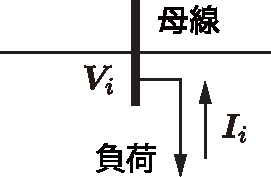
\includegraphics[width = .25\linewidth]{figs/loadbus}
  \medskip
  \caption{\textbf{Load connected to bus bar}}
  \label{fig:loadbus}
  \medskip
\end{figure}

With regard to static load models, \textbf{constant impedance model},
\textbf{constant power model}, and \textbf{constant current model} or
combinations of them are often used. These are all static models described by
algebraic equations with respect to the current and voltage phasors. Let us
assume that voltage phasor of a bus bar $i$ connected with a load is $\bm{V}_i$
and the current phasor flowing from the load to the bus bar is $\bm{I}_i$
(\ref{fig:loadbus}). Then, the constant impedance model is given by the
following relationship:

\begin{subequations}\label{eq:ldynVI}
\begin{equation}\label{eq:cimp}
  \bm{I}_i= - \frac{ \bm{V}_i}{\bm{z}_{{\rm load}i}^{\star}}
\end{equation}
where, $\bm{z}_{{\rm load}i}^{\star} \in \mathbb{C}$ is a constant expressing
the impedance of the load.

The negative sign on the right side of Equation \ref{eq:cimp} indicates the load
is grounded and the direction of the flow of thecurrent phasor $\bm{I}_i$ from
the load to the bus bar $i$ is defined as positive. Specifically:

\[
  \bm{I}_i= \frac{1}{\bm{z}_{{\rm load}i}^{\star}} (0-\bm{V}_i)
\]

Incandescent lamps and electric heaters are common devices that can be expressed
by the constant impedance model.

The constant current model is expressed by the following relationship, where
$\bm{I}_{{\rm load}i}^{\star} \in \mathbb{C}$ is a constant current phasor.

\begin{equation}\label{eq:ccrt}
  \bm{I}_i = \bm{I}_{{\rm load}i}^{\star} e^{\bm{j} \angle \bm{V}_i }
\end{equation}

In other words, the following is true for the magnitude $|\bm{I}_{{\rm
load}i}^{\star}|$ and phase $\angle \bm{I}_{{\rm load}i}^{\star}$:

\[
  |\bm{I}_i| = |\bm{I}_{{\rm load}i}^{\star}|,\qquad
  \angle \bm{I}_i = \angle \bm{I}_{{\rm load}i}^{\star} + \angle \bm{V}_i
\]

The constant power model is given by the following relationship:
\begin{equation}\label{eq:cpw}
  \bm{I}_i = \frac{P_{{\rm load}i}^{\star} - \bm{j} Q_{{\rm load}i}^{\star} }{\overline{\bm{V}}_i}
\end{equation}
\end{subequations}
where $P_{{\rm load}i}^{\star} \in \mathbb{R}$ and $Q_{{\rm load}i}^{\star} \in
\mathbb{R}$ are constant active and reactive power supplied to the bus bar $i$.
This is derived by considering the complex conjugate of:

\[
  P_{{\rm load}i}^{\star} + \bm{j} Q_{{\rm load}i}^{\star} =
  \bm{V}_i \overline{\bm{I}}_i
\]

Power converters can be represented as constant-current models or constant power
model, depending on their characteristics.

Depending on the purpose of the analysis, a dynamic load model might be used.
Please see \cite[Section 7.1.2]{kundur1994power} for further details.

\subsection{Kron reduction of load bus bar}

Even when there are generators and multiple types of loads connected in a power
system, a mathematical model of the system can be obtained by defining the
relationship between the current and voltage phasors of each device using
Equations \ref{eq:gendynVI} and \ref{eq:ldynVI} and combining them with Equation
\ref{eq:ohmY}. In this case, the constant impedance model in Equation
\ref{eq:cimp} gives a linear relationship between the current and voltage
phasors. On the other hand, the constant-current model in Equation \ref{eq:ccrt}
and the constant-power model in Equation \ref{eq:cpw} provide nonlinear
relationships for current and voltage phasors, which generally makes
mathematical analysis of the resulting power system model difficult. Let us
illustrate this fact with the following example.

\begin{example}{Kron reduction of load bus bar}\label{ex:genloadY} 
  
Let us assume that in the electrical power system of the Example \ref{ex:derY},
the generators are represented by devices 1 and 2, and the load is represented
by device 3. The relationship between current and voltage phasors and the
admittance matrix of the power grid is given by Equation \ref{eq:exY}. First,
let us consider the case where the load is given by the constant impedance
model.  If $\bm{z}_{{\rm load}3}^{\star}$ is the impedance of the load, the
following Equation can be obtained:

\[
  \bm{I}_3 = -\frac{ \bm{V}_3}{\bm{z}_{{\rm load}3}^{\star}}
\]

If this is substituted into Equation \ref{eq:exY} to cancel $\bm{I}_3$:

\begin{equation}\label{eq:exYcimp}
  \mat{
    \bm{I}_1\\
    \bm{I}_2\\
    0\\
  }
  =
  \mat{
    \bm{y}_{12} & -\bm{y}_{12} & 0\\
    -\bm{y}_{12} & \bm{y}_{12}+\bm{y}_{32} & -\bm{y}_{32}\\
    0 & -\bm{y}_{32} & \bm{y}_{32}  + \tfrac{1}{\bm{z}_{{\rm load}3}^{\star}}
  }
  \mat{
    \bm{V}_1\\
    \bm{V}_2\\
    \bm{V}_3\\
  }
\end{equation}

Please note that with the equation on the third row the voltage phasor
$\bm{V}_3$ can be written in function of the voltage phasor $\bm{V}_2$ of the
generator bus. Specifically:

\begin{equation*}
  \bm{V}_3 = \left(\bm{y}_{32} + \tfrac{1}{\bm{z}_{{\rm load}3}^{\star}} \right)^{-1} \bm{y}_{32} \bm{V}_2
\end{equation*}

In addition, by replacing $\bm{V}_3$ using the above expression, the
relationship between the current and voltage phasors of the generator bus bar
group becomes:

\begin{equation*}
  \mat{
    \bm{I}_1\\
    \bm{I}_2
  }
  =
  \bm{Y}_{\rm Kron}
  \mat{
    \bm{V}_1\\
    \bm{V}_2\\
  }
\end{equation*}

The reduced admittance matrix of the load bus bar is obtained as:

\[
  \bm{Y}_{\rm Kron}:=
  \mat{
    \bm{y}_{12} & -\bm{y}_{12}\\
    -\bm{y}_{12} & \bm{y}_{12}+\bm{y}_{32}
  }
  -
  \mat{
    0\\
    \bm{y}_{32}
  }
  \left( 
  \bm{y}_{32} 
  + \tfrac{1}{\bm{z}_{{\rm load}3}^{\star}} 
  \right)^{-1}
  \mat{
    0&\bm{y}_{32}
  }
\]
Therefore, if the load is given as a constant impedance model, the load busbar
and its variables can be eliminated by considering $\bm{Y}_{\rm Kron} \in
\mathbb{C}^{2\times 2}$ as the admittance matrix of the new power grid, and the
system can be equivalently transformed into a system of differential algebraic
equations with only the generator connected to the busbar.

Next, let us consider a situation where the load is given as the constant
current model. Let us assume that current phasor flows from the load to bus bar
3:
\[
  \bm{I}_3 = \bm{I}_{{\rm load}3}^{\star} e^{\bm{j} \angle \bm{V}_3}
\]

Then, following the same procedure as for the constant impedance model, and
replacing $\bm{I}_3$ and $\bm{V}_3$ in Equation \ref{eq:exY}, the following is
obtained:

\begin{equation*}
  \mat{
    \bm{I}_1\\
    \bm{I}_2
  }
  =
  \bm{Y}_{\rm Kron}'
  \mat{
    \bm{V}_1\\
    \bm{V}_2\\
  }
  +
  \mat{
    0\\
    -\bm{y}_{32}
  }
  \bm{y}_{32}^{-1}
  \bm{I}_{{\rm load}3}^{\star} e^{\bm{j} \angle \bm{V}_3}
\end{equation*}

where:

\[
  \bm{Y}_{\rm Kron}' :=
  \mat{
    \bm{y}_{12} & -\bm{y}_{12}\\
    -\bm{y}_{12} & \bm{y}_{12}+\bm{y}_{32}
  }
  -
  \mat{
    0\\
    \bm{y}_{32}
  }
  \bm{y}_{32}^{-1}
  \mat{
    0&\bm{y}_{32}
  }
\]

This means that, if the load is given as the constant current model, the
relationship between the current and voltage phasors of the generators is
affine. However, the phase $\angle \bm{V}_3$ of the voltage phasor of the load
bus bar also has an impact on the current phasor of the generators. Generally,
the phase $\angle \bm{V}_3$ of the voltage phasor is a nonlinear function of the
voltage phasor $\bm{V}_3$.

Finally, let us consider a case wherein the load is given as the constant power
model. When constant active power $P_{{\rm load}3}^{\star}$ and reactive
power $Q_{{\rm load}3}^{\star}$ are supplied from the load to bus bar 3, the
following relationship holds:

\begin{equation*}
  \bm{I}_3 = \frac{P_{{\rm load}3}^{\star} - \bm{j} Q_{{\rm load}3}^{\star} }{\overline{\bm{V}}_3}
\end{equation*}

Since this is a nonlinear relationship of $\bm{I}_3$ and $\bm{V}_3$, to cancel
$\bm{V}_3$ from Equation \ref{eq:exY}, nonlinear calculation is necessary.
Specifically, $\bm{V}_3$ is given as a solution for the quadratic equation
related to complex variables:

\begin{equation*}
  \bm{y}_{32} \bm{V}_3 \overline{\bm{V}}_3 - \bm{y}_{32}  \bm{V}_2 \overline{\bm{V}}_3 -P_{{\rm load}3}^{\star} 
  + \bm{j} Q_{{\rm load}3}^{\star} =0
\end{equation*}

Therefore, if the load of the constant power model is included in an electrical
power system model, it is usually difficult to cancel the load bus bar through
equivalent transformation.

\end{example}

As shown in Example \ref{ex:genloadY}, if the load is given as a static model
expressed by Equation (\ref{eq:ldynVI}), the current phasor and voltage phasor
of some or all load bus bars can be equivalently cancelled through algebraic
calculation. This operation is called \textbf{Kron reduction of the load bus
bar}. Specifically, when the load is given as the constant impedance model,
Kron reduction of the load bus bar corresponds to reducing the dimension of the
admittance matrix of the power grid by mathematically equivalent calculation.

If there is no device connected to the bus bar, such as a generator or load,
we can assume a constant impedance model load with an infinite absolute value of
$\bm{z}_{{\rm load}i}^{\star}$ connected to bus $i$ in Equation \ref{eq:cimp}.
This is equivalent to a virtual connection of a constant-current model load in
which the current phasor between the load and the bus is always zero. Therefore,
the above-described Kron reduction of the load bus bar allows for equivalent
cancellation of bus bars without device.


\subsection{Mathematical properties of the admittance matrix with reduced load
bus bar}

Let us analyze properties that hold for Kron reduction of the load bus bar when
all loads are given by the constant impedance model. First, the procedure for
Kron reduction in Example \ref{ex:genloadY} is shown as a general form when the
number of generator and load buses is arbitrary. The subscripts set of
generator buses is $\mathcal{I}_{\rm G}$ and the subscripts set of load bus bars
is $\mathcal{I}_{\rm L}$. Without loss of generality, the number of generator
buses is assumed to be inferior to that of load buses. In other words:

\begin{equation*}
  \mathcal{I}_{\rm G} = \{ 1,\ldots, n \},\qquad
  \mathcal{I}_{\rm L} = \{ n+1,\ldots, n + m \}
\end{equation*}
where $n$ and $m$ are numbers of generator buses and load bus bars, respectively.
By definition, $n+m$ is equal to the total number of bus bars $N$.

Let $\bm{I}_{\rm G} \in \mathbb{C}^{n}$ be the vector of current phasors of all
generator buses, and $\bm{V}_{\rm G} \in \mathbb{C}^{n}$ be the vector of
voltage phasors. Similarly, the vector of current phasors of all load buses is
expressed as $\bm{I}_{\rm L}\in \mathbb{C}^{m}$, and the vector of voltage
phasors is expressed as $\bm{V}_{\rm L} \in \mathbb{C}^{m}$. Then, the
relationship between all current and voltage phasors with respect to the
admittance matrix $\bm{Y}\in \mathbb{C}^{N\times N}$ of the power grid is:

\begin{equation}\label{eq:YGL}
  \mat{
    \bm{I}_{\rm G}\\
    \bm{I}_{\rm L}
  }
  =
  \underbrace{
    \mat{
      \bm{Y}_{\rm GG} & \bm{Y}_{\rm GL}\\
      \bm{Y}_{\rm LG} & \bm{Y}_{\rm LL}
    }
  }_{\bm{Y}}
  \mat{
    \bm{V}_{\rm G}\\
    \bm{V}_{\rm L}
  }
\end{equation}

Here, the relationship between the current phasor and the voltage phasor
determined by the load in the constant impedance model is expressed using the
admittance:

\begin{equation*}
  \bm{I}_{\rm L}=- \sfdiag(\bm{y}_{{\rm load}i}^{\star} )_{i \in \mathcal{I}_{\rm L}}\bm{V}_{\rm L}
\end{equation*}

Although $\bm{y}_{{\rm load}i}^{\star}$ is defined as a reciprocal of
$\bm{z}_{{\rm load}i}^{\star}$ in Equation \ref{eq:cimp} and must have a
non-zero value, since this is an expression of bus bars with no equipment
connected, formally, $\bm{y}_{{\rm load}i}^{\star}$ is allowed to be 0.
Substituting it in Equation \ref{eq:YGL} to cancel $\bm{V}_{\rm L}$, the
followed is obtained.

\begin{equation}\label{eq:Kron}
  \bm{I}_{\rm G} = 
    \Bigl\{ 
      \underbrace{
        \bm{Y}_{\rm GG} - \bm{Y}_{\rm GL} 
        \bigl( \bm{Y}_{\rm LL} + \sfdiag(\bm{y}_{{\rm load}i}^{\star} )_{i \in \mathcal{I}_{\rm L}} \bigr)^{-1}
        \bm{Y}_{\rm LG} 
      }_{\bm{Y}_{\rm Kron}}
    \Bigr\}
  \bm{V}_{\rm G}
\end{equation}

Note that in general, if the load consumes active and reactive power with
respect to the admittance of the load, then the following holds as in
transmission lines.

\begin{equation}\label{eq:loadys}
  \operatorname{Re}[\bm{y}_{{\rm load}i}^{\star} ] \geq 0 ,\qquad
  \operatorname{Im}[\bm{y}_{{\rm load}i}^{\star} ] \leq 0
  ,\qquad
  \forall i \in \mathcal{I}_{\rm L}
\end{equation}

In addition, the conductance and susceptance matricces obtained by Kron
reduction of the load bus, which are the real and imaginary parts of
$\bm{Y}_{\rm Kron}$, are expressed as:

\[
  G_{\rm Kron} := \real \bigl[  \bm{Y}_{\rm Kron}  \bigr] ,\qquad
  B_{\rm Kron} := \imag \bigl[  \bm{Y}_{\rm Kron}  \bigr]
\]
This introduces the following fact:

\begin{theorem}[Properties of the Kron-reduced admittance matrix]
\label{thm:Kron}
For the admittance matrix $\bm{Y}\in \mathbb{C}^{N\times N}$ of Equation
\ref{eq:Ypig}, by dividing the block matrix of Equation \ref{eq:YGL},
$\bm{Y}_{\rm Kron}\in \ \mathbb{C}^{n\times n}$ of Equation \ref{eq:Kron} can be
obtained, corresponding to the admittance matrix of the system after the Kron
reduction of the load bus bars. Additionally, the admittance $\bm{y}_{{\rm
load}i}^{\star} $ of each load satisfies Equation \ref{eq:loadys}.  Then, the
reduced conductance matrix $G_{\rm Kron}$ is positive semi-definite, and the
reduced susceptance matrix $B_{\rm Kron}$ is symmetric. Furthermore, if the following
is true for the generator buses:

\begin{subequations}\label{eq:betas}
\begin{equation}\label{eq:betag}
  \Cgi = 0
  ,\qquad
  \forall i \in \mathcal{I}_{\rm G}
\end{equation}

And the following is true for load bus bars:

\begin{equation}\label{eq:betay}
  \operatorname{Im}[\bm{y}_{{\rm load}i}^{\star} ] + \Cgi \leq 0
  ,\qquad
  \forall i \in \mathcal{I}_{\rm L}
  \end{equation}
\end{subequations}
where $\Cgi$ is a non-negative constant equivalent to the capacitance to ground
of Equation \ref{eq:Ypig}, $B_{\rm Kron}$ is negative semidefinite.   

Specifically, if the inequality of Equation \ref{eq:betay} strictly holds for at
least one load bus bar, then $B_{\rm Kron}$ is negative definite.
\end{theorem}

\begin{proof}

Using Lemma \ref{lem:schur} of the Mathematical Supplement at the end of the
chapter, let us define:

\begin{equation*}
  \bm{Y}' := 
  \mat{
  \bm{Y}_{\rm GG} & \bm{Y}_{\rm GL}\\
  \bm{Y}_{\rm LG} & \bm{Y}_{\rm LL} +\sfdiag(\bm{y}_{{\rm load}i}^{\star} )_{i \in \mathcal{I}_{\rm L}}
  }
\end{equation*}

Since Equations \ref{eq: Y0} and \ref{eq: loadys} hold, the real part of $\bm{j}
\bm{Y}'$ is symmetric, and the imaginary part is positive semidefinite.
Therefore, Lemma \ref{lem:schur} shows that the real part of $\bm{j} \bm{Y}_{\rm
Kron} $ is symmetric and the imaginary part is semi-positive. This implies that
the real part of $\bm{Y}_{\rm Kron}$, $G_{\rm Kron}$, is positive semidefinite
and the imaginary part, $B_{\rm Kron}$, is symmetric.

Moreover, when Equation \ref{eq:betas} holds, the imaginary part of $\bm{Y}'$ is
negative semidefinite, which by the Lemma \ref{lem:schur} implies that $B_{\rm
Kron}$ is negative semidefinite. Similarly, if Equation \ref{eq:betay} holds
strictly for at least one load bus bar, then $\bm{Y}'$ and $B_{\rm Kron}$ are
negative definite.

\end{proof}

Theorem \ref{thm:Kron} shows that, if all loads are given by the constant
impedance model, the conductance and susceptance matrix of related to the
admittance matrix of Equation \ref{eq:Ypig} remain positive semidefinite and
symmetric, respectively, even if the load bus bars were Kron reduced.
Therefore, it can be similarly applied to the electrical power system model, in
which the generator buses and load bus bars in Section \ref{sec:allgen} are Kron
reduced. Theorem \ref{thm:Kron} shows a case where all load bus bars are Kron
reduced simultaneously. However, the same fact is shown when only some of load
bus bars are Kron reduced.

As discussed above, while the definiteness of the admittance matrix is
invariable to Kron reduction, the "element signs" of the real and imaginary
parts are not necessarily invariable. Let us confirm this with the next Example.

\begin{example}{Sign change of the admittance matrix by Kron reduction of bus
bars}\label{ex:kronsign}

Regarding the admittance matrix $\bm{Y}_0$ when the ground capacitance in
Equation \ref{eq:Y0prop} is negligible, the conductance matrix $G_0$ is positive
semidefinite and the susceptance matrix $B_0$ is negative semidefinite. Then,
the diagonal and non-diagonal elements of $G_0$ are non-negative and
non-positive, respectively, and the diagonal and non-diagonal elements of $B_0$
are non-positive and non-negative, respectively. For example, For example, let
bus 1 and bus 2 be the generator bus, bus 3 be the load bus. Then, the load bus
admittance and the power grid admittance matrix are:

\begin{equation*}
  \bm{y}_{{\rm load}3}^{\star} = \alpha - \bm{j} \beta 
  ,\qquad
  \bm{Y}=  
  \underbrace{
    \gamma \mat{
      1&-1&0\\
      -1&1&0\\
      0&0&0
    }
  }_{G_0}+
  \bm{j} 
  \underbrace{
    \mat{
      -2&1&1\\
      1&-2&1\\
      1&1&-2
    }
  }_{B_0}
\end{equation*}
where $\alpha$, $\beta$, and $\gamma$ are non-negative constants.
Please note that the signs of the real and imaginary parts of the load bus
admittance of are the same as the signs of the diagonal element of the
admittance matrix. 

By Kron reducing the load bus bar, the reduced admittance matrix of Equation
\ref{eq:Kron} becomes:

\begin{equation*}
  \spliteq{
    & \bm{Y}_{\rm Kron}
    = 
    \underbrace{
      \gamma
      \mat{
        1&-1\\
        -1&1\\
      }
      +
      \frac{\alpha}{\alpha^2 + (2+\beta)^2}
      \mat{
        1&1\\
        1&1\\
      }
    }_{G_{\rm Kron}}
    \\
    & \hspace{7em} +
    \bm{j} 
    \underbrace{
      \left(
      \mat{
        -2&1\\
        1&-2\\
      }
      +
      \frac{2+\beta}{\alpha^2 + (2+\beta)^2}
      \mat{
        1&1\\
        1&1\\
      }
      \right)
      }_{B_{\rm Kron}}
  }
\end{equation*}

Here, for arbitrary non-negative constants, $\alpha$, $\beta$, and $\gamma$, the
diagonal element of $G_{\rm Kron}$ is non-negative and the diagonal and
non-diagonal elements of $B_{\rm Kron}$ are negative and positive, respectively.
However, the non-diagonal element of $G_{\rm Kron}$ is positive when:

\begin{equation*}
  \gamma < \frac{\alpha}{\alpha^2 + (2+\beta)^2} 
\end{equation*}

Thus, when the laod bus bar is Kron reduced, the sign of the non-diagonal
elements of the admittance matrix is not always invariable. The diagonal
elements are invariable because of t he positive semidefinite nature of $G_0$
and the negative semidefinite nature of $B_0$.

A change of sign of an off-diagonal element can occur when the conductance and
susceptance are both non-zero for the load or transmission line connected to the
bus bar being Kron reduced. For example, in the above case, the admittance of
the load is a pure imaginary number when $\alpha=0$ and the admittance of the
transmission line connected to bus bar 3; in other words, the elements of the
third column and the third row of $\bm{Y}$, are all pure imaginary. In such a
case, it can be shown that there is no sign change of the elements of the
conductance and susceptance matrices.

\end{example}

The above-described Kron reduction has been known as a mathematical operation
related to the derivation of an equivalent circuit \cite{kron1939tensor}.
Specifically, in the analysis of an electrical power system, it is applied to
power flow calculations explained in Section \ref{sec:howtocal}. Kron reduction
has also been applied in graph theory, and has interesting mathematical
properties \cite{dorfler2013kron}.


%\section{蓄電池の数理モデル?}
%
%\section{再エネの数理モデル?}

%\bibliographystyle{myjunsrt}		% bib style
%\bibliography{reference}	% your bib database


\section*{Mathematical Supplement}
\begin{lemma}\label{lem:nonsing}
Assume that the real matrix $M$ is regular. Then, for real matrix $N$, the necessary
and sufficient condition for $M + jN$ to be regular is that $M + NM-1N$ is regular.
\end{lemma}

\begin{proof}
First, the fact that $M+ \bm{j} N$ is regular is equivalent to the fact that
there exist certain real square matrices $P$ and $Q$ such that $(M+ \bm{j} N)(P+
\bm{j} Q)=I$. If we rearrange these two equations for the real and imaginary
parts, we get:

\begin{equation}\label{eq:MNinv}
  \underbrace{
  \mat{
    M & -N\\
    N & M
  }
  }_{L}
  \mat{
    P & -Q\\
    Q & P
  }
  =I
\end{equation}

This means that the regularity of $M+ \bm{j} N$ is equivalent to the regularity
of $L$. Furthermore, using the properties of the determinant of block matrices:

\begin{equation*}
  \sfdet L =\sfdet M \sfdet \left(M+NM^{-1}N\right)
\end{equation*}

From the assumption that $\sfdet M \neq 0$, the regularity of $L$ is equivalent
to the regularity of $M+NM^{-1}N$. Then, the lemma is proven to be true. 
\end{proof}

\begin{lemma}\label{lem:sdreim}
Let the real part of the complex matrix $\bm{Z}$ be positive definite. If the
imaginary part of $\bm{Z}$ is symmetric, then the real part of $\bm{Z}^{-1}$ is
positive definite and the imaginary part is symmetric. In particular, if the
imaginary part of $\bm{Z}$ is positive semidefinite, then the imaginary part of
$\bm{Z}^{-1}$ is negative semidefinite. Also, if the imaginary part of $\bm{Z}$
is positive definte, the imaginary part of $\bm{Z}^{-1}$ is negative definite.
\end{lemma}

\begin{proof}
Let $\bm{Z} = M + \bm{j} N$, where $M$ is a real positive definite matrix and
$N$ is a symmetric matrix. Let $P$ be the real part of $\bm{Z}^{-1}$ and $Q$ be
its imaginary part. From the Lemma \ref{lem:nonsing}, $M+NM^{-1}N$ is positive
definite and therefore $\bm{Z}$ is regular. Therefore

\[
  (M+ \bm{j} N)(P+ \bm{j} Q)=I
\]

The equations for the real and imaginary parts of $L$ are equivalent to the Equation \ref{eq:MNinv}.
This means that the diagonal and off-diagonal blocks of the inverse of $L$ are $P$ and $Q$.
From the properties of the inverse of the block matrix
\begin{equation*}
L^{-1}=
\mat{
(M+NM^{-1}N)^{-1} & M^{-1}N(M+NM^{-1}N)^{-1} \\
-(M+NM^{-1}N)^{-1}NM^{-1} & (M+NM^{-1}N)^{-1}
}
\end{equation*}

Therefore,
\begin{equation*}
P=(M+NM^{-1}N)^{-1},\qquad
Q=-M^{-1}N(M+NM^{-1}N)^{-1}
\end{equation*}
From the assumption that $N$ is symmetric and $M$ is positive definite, $P$ is positive definite.
Also, using the positive definite matrix $\sqrt{M^{-1}}$ such that $M^{-1}=\sqrt{M^{-1}}\sqrt{M^{-1}}$, $Q$ is
\begin{equation*}
Q=-\sqrt{M^{-1}} 
\underbrace{
\sqrt{M^{-1}} N \sqrt{M^{-1}}
\left(
I + (\sqrt{M^{-1}} N \sqrt{M^{-1}} )^2
\right)^{-1}
}_{X}
\sqrt{M^{-1}}
\end{equation*}
where $\sqrt{M^{-1}} N \sqrt{M^{-1}}$ is symmetric, so it can be diagonalized by the orthogonal matrix $V$ and
\begin{equation*}
X = V \Lambda \left(
I + \Lambda^2
\right)^{-1}
V^{\sf T}
\end{equation*}
However, $\Lambda$ is a real diagonal matrix of eigenvalues of $\sqrt{M^{-1}} N \sqrt{M^{-1}}$.
From this, since $X$ is symmetric, $Q$ is also symmetric.
Furthermore, if $N$ is semi-definite, then $\Lambda$ is also semi-definite, and if $N$ is positive, then $\Lambda$ is also positive.
Therefore, if $N$ is semi-positive definite, then $Q$ is semi-negative definite, and if $N$ is positive definite, then $Q$ is negative definite.
From the above, the subject follows.
\end{proof}



\begin{lemma}\label{lem:schur}
\red{Translated with DeepL}
Consider symmetric running matrices $M$ and $N$.
They are partitioned into block matrices
\begin{equation}\label{eq:defbmZ}
\mat{
\bm{Z}_{11} & \bm{Z}_{12} \\
\bm{Z}_{21} & \bm{Z}_{22}
}
:=
\underbrace{
\mat{
M_{11} & M_{12} \\ 
M_{12}^{\sfT} & M_{22}
}
}_{M}
+\bm{j}
\underbrace{
\mat{
N_{11} & N_{12} \\ 
N_{12}^{\sfT} & N_{22}
}
}_{N}
\end{equation}
For $\bm{Z}_{11} - \bm{Z}_{12}\bm{Z}_{22}^{-1}\bm{Z}_{21}$ denote $\bm{Z}_{\rm S}$.
Also assume that $M$ is semi-definite and that $M_{22}$ is positive definite.
In this case, the real part of $\bm{Z}_{\rm S}$ is semipositive definite and the imaginary part is symmetric.
In particular, if $N$ is semipositive definite, then the imaginary part of $\bm{Z}_{\rm S}$ is semipositive definite.
Also, if $N$ is positive definite, then the imaginary part of $\bm{Z}_{\rm S}$ is positive definite.
Furthermore, if $M$ is positive definite, then the real part of $\bm{Z}_{\rm S}$ is positive definite.
\end{lemma}

\begin{proof}
\red{Translated with DeepL}
Denote by $\bm{Z}$ the matrix on the left-hand side of the Equation \ref{eq:defbmZ}.
First, if $M$ is positive definite, then the real part of $\bm{Z}_{\rm S}$ is positive definite and the imaginary part is symmetric.
Now, from the positive definiteness of $M_{22}$, $\bm{Z}_{22}$ is regular from the complement \ref{lem:nonsing}.
Therefore, by the inverse property of the block matrix, $\bm{Z}_{\rm S}^{-1}$ coincides with the upper left block of $\bm{Z}^{-1}$.
Here, from the complementation\ref{lem:sdreim}, the real part of $\bm{Z}^{-1}$ is positive definite and the imaginary part is symmetric.
This means that the real part of $\bm{Z}_{\rm S}^{-1}$ is positive definite and the imaginary part is symmetric.
Therefore, applying the complementation \ref{lem:sdreim} to $\bm{Z}_{\rm S}^{-1}$ shows that the real part of $\bm{Z}_{\rm S}$ is positive definite and the imaginary part is symmetric.
Similarly, if $N$ is semipositive definite, then from the complementation \ref{lem:sdreim}, the imaginary part of $\bm{Z}^{-1}$ is semidefinite, which means that the imaginary part of $\bm{Z}_{\rm S}^{-1}$ is semidefinite.
Therefore, by applying the complementation \ref{lem:sdreim} again to $\bm{Z}_{\rm S}^{-1}$, it can be shown that the imaginary part of $\bm{Z}_{\rm S}$ is semipositive definite.


Next, consider the case where $M$ is semidefinite and $N$ is symmetric.
First, show that both the real and imaginary parts of $\bm{Z}_{\rm S}$ are symmetric.
Now, since the real part $M_{22}$ of $\bm{Z}_{22}$ is positive definite and the imaginary part $N_{22}$ is symmetric, both real and imaginary parts of $\bm{Z}_{22}^{-1}$ are symmetric.
Therefore,
\begin{equation*}
\spliteq{
\real [\bm{Z}_{\rm S} ] &= \real [\bm{Z}_{11} ]
- \real [\bm{Z}_{12} ] \real [\bm{Z}_{22}^{-1} ] \real [\bm{Z}_{21} ]\\
&+ \imag [\bm{Z}_{12} ] \imag [\bm{Z}_{22}^{-1} ] \real [\bm{Z}_{21} ]
+ \imag [\bm{Z}_{12} ] \real [\bm{Z}_{22}^{-1} ] \imag [\bm{Z}_{21} ] \\
&+ \real [\bm{Z}_{12} ] \imag [\bm{Z}_{22}^{-1} ] \imag [\bm{Z}_{21} ]\\
&= M_{11} - M_{12}  \real [\bm{Z}_{22}^{-1} ] M_{12}^{\sfT} 
+ N_{12}  \imag [\bm{Z}_{22}^{-1} ] M_{12}^{\sfT} 
+ N_{12}  \real [\bm{Z}_{22}^{-1} ] N_{12}^{\sfT} \\
&+ M_{12}  \imag [\bm{Z}_{22}^{-1} ] N_{12}^{\sfT}
}
\end{equation*}
From this we see that the real part of $\bm{Z}_{\rm S}$ is symmetric.
Similarly,
\begin{equation*}
\spliteq{
\imag [\bm{Z}_{\rm S} ]& = N_{11} + N_{12}  \imag [\bm{Z}_{22}^{-1} ] N_{12}^{\sfT} 
- N_{12}  \real [\bm{Z}_{22}^{-1} ] M_{12}^{\sfT} \\
& - M_{12}  \imag [\bm{Z}_{22}^{-1} ] M_{12}^{\sfT} 
- M_{12}  \real [\bm{Z}_{22}^{-1} ] N_{12}^{\sfT}
}
\end{equation*}
From this we see that the imaginary part of $\bm{Z}_{\rm S}$ is also symmetric.

When $M$ in the expression \ref{eq:defbmZ} is semi-definite, $\bm{Z}$ is not necessarily regular, since $\bm{Z}^{-1}$ is not necessarily regular.
In contrast, in what follows, for any $\epsilon >0$:
\begin{equation*}
\bm{Z}^{+}
:=
\mat{
\bm{Z}_{11}+ \epsilon I & \bm{Z}_{12} \\
\bm{Z}_{21} & \bm{Z}_{22}+ \epsilon I
}
\end{equation*}
The real part of $N$, $M+\epsilon I$, is positive definite.
Now, when $N$ is semi-definite, for any $\epsilon >0$ we have
\begin{equation*}
\bm{Z}_{\rm S}^{+}:=\bm{Z}_{11} + \epsilon I - \bm{Z}_{12} (\bm{Z}_{22}+ \epsilon I)^{-1}\bm{Z}_{21}
\end{equation*}
The real part of $(\bm{Z}_{22}+ \epsilon I)^{-1}$ is positive definite, and the imaginary part is semi-positive definite.
Also, by expanding $(\bm{Z}_{22}+ \epsilon I)^{-1}$ using the auxiliary theorem of the inverse matrix the following is obtained.
\begin{equation*}
\bm{Z}_{\rm S}^{+}=
\bm{Z}_{\rm S}
+ \underbrace{
\epsilon
\left\{
I + \bm{Z}_{12} \bm{Z}_{22}^{-1}
(I +\epsilon \bm{Z}_{22}^{-1} )^{-1}
\bm{Z}_{22}^{-1}\bm{Z}_{21}
\right\}
}_{\Delta(\epsilon)}
\end{equation*}
As mentioned above, since the real and imaginary parts of $\bm{Z}_{\rm S}^{+}$ and $\bm{Z}_{\rm S}$ are symmetric,
the real and imaginary parts of $\Delta(\epsilon)$ are also symmetric.

Next, we show that the imaginary part of $\bm{Z}_{\rm S}^{+}$ is semipositive definite if and only if $\bm{Z}_{\rm S}$ is semipositive definite.
Note that the same argument can be used to show the semi- positive definiteness of the real part.
For the following discussion
\begin{equation*}
\mathcal{X} := \left\{
x: 
x^{\sf T} \imag[\Delta (\epsilon)] x >0
,\quad 
\forall \epsilon >0
\right\}
\end{equation*}
is defined as follows.
From this definition of $\mathcal{X}$, for arbitrarily chosen $x \notin \mathcal{X}$, there exists some $\epsilon_0 >0$ such that
\[
x^{\sf T} \imag[\Delta(\epsilon_0)]x \leq 0
\]
Therefore, the imaginary part of $ \bm{Z}_{\rm S}^{+} $ is semi-positive definite, 
\begin{equation*}
x^{\sf T} \imag [\bm{Z}_{\rm S}] x + x^{\sf T} \imag[\Delta(\epsilon_0)]x \geq 0
\end{equation*}
is derived.
This leads to the following for all $x \notin \mathcal{X}$, 
\begin{equation}\label{eq:xZxgeq}
x^{\sf T}\imag[\bm{Z}_{\rm S}] x \geq 0
\end{equation}

Furthermore, if the imaginary part of $ \bm{Z}_{\rm S}^{+} $ is semi-positive definite, we show by contraposition that the expression \ref{eq:xZxgeq} holds for all $x \in \mathcal{X}$.
That is, for some $x \in \mathcal{X}$, we have
\begin{equation}\label{eq:xZxleq}
x^{\sf T} \imag[\bm{Z}_{\rm S}] x < 0
\end{equation}
then the imaginary part of $ \bm{Z}_{\rm S}^{+} $ is not semidefinite.
Now, noting that the imaginary part of $\Delta(\epsilon)$ asymptotes to 0 in the limit of $\epsilon \rightarrow 0$, if for some $x \in \mathcal{X}$ the expression\ref{eq:xZxleq}
\begin{equation*}
x^{\sf T} \imag[ \bm{Z}_{\rm S}] x 
+
x^{\sf T} \imag[\Delta(\epsilon_0)]x < 0
\end{equation*}
This means that the imaginary part of $\bm{Z}_{\rm S}^{+} $ is not semi- positive definite.
The above facts show that the imaginary part of $\bm{Z}_{\rm S}$ is semi-positive definite.

Finally, we show that if $N$ is positive definite, then the imaginary part of $\bm{Z}_{\rm S}$ is positive definite.
For this purpose, 
\begin{equation*}
-\bm{j} \bm{Z} = N - \bm{j} M
\end{equation*}
is positive definite and the imaginary part is symmetric.
Applying the results for the case where the real part is positive definite to this $-\bm{j} \bm{Z}_{\rm S}$, it can be shown that the real part of $-\bm{j} \bm{Z}_{\rm S}$ is positive definite.
This implies that the imaginary part of $\bm{Z}_{\rm S}$ is positive definite.
\end{proof}


%\newpage
\end{document}